%_______________________________________________________________________________
%class
%_______________________________________________________________________________
%\documentclass[a4paper,11pt,onecolumn,final,german,openbib]{scrbook}
\documentclass[a4paper,11pt,twosided,final,german,openbib,pdftex,listof=totoc,bibliography=totoc]{scrbook}
%_______________________________________________________________________________
% page borders
%_______________________________________________________________________________
\addtolength{\headheight}{2cm}
%\addtolength{\topmargin}{2cm}
\setlength{\oddsidemargin}{1.0cm}
\setlength{\evensidemargin}{0.5cm}
\setlength{\textwidth}{14.3cm}
\setlength{\parindent}{0mm}

%_______________________________________________________________________________
% packages
%_______________________________________________________________________________
\usepackage[english]{babel}
\usepackage{amsmath, amssymb}
\usepackage[utf8]{inputenc}
\usepackage{graphicx}
\usepackage{enumerate}
\usepackage{enumitem}
\usepackage{multirow}
\usepackage{subfigure}
\usepackage{dsfont}
\usepackage{slashed}
\usepackage{textcomp}
\usepackage{url}
\usepackage{amsmath}
\usepackage{hyperref}
\usepackage{caption}
\usepackage{wrapfig}
\usepackage{nicefrac}
\usepackage[backend=bibtex,style=numeric,sorting=none]{biblatex}
\usepackage{lmodern}
\usepackage{epigraph}
\usepackage[T1]{fontenc}
\usepackage{yfonts,color}
\usepackage{titlesec}
\usepackage{lettrine}
\usepackage{fancyhdr}
\usepackage{verbatim}
\usepackage[compat=1.0.0]{tikz-feynman}
\usepackage{tikz}
\usetikzlibrary{decorations.pathmorphing,decorations.markings,trees}
\usepackage{afterpage}
\usepackage{listings}
\usepackage{float}
\usepackage{scrextend}
\usepackage{titling}
\floatstyle{plaintop}
\restylefloat{table}
\maxdeadcycles=1000

\lstset{
	numbers=left,               % Ort der Zeilennummern
	stepnumber=2,               % Abstand zwischen den Zeilennummern       
	numberfirstline=false,
	basicstyle=\ttfamily,
	columns=fullflexible,
	frame=single,
	breaklines=true,
	postbreak=\mbox{\textcolor{red}{$\hookrightarrow$}\space},
}



\newcommand\blankpage{%
	\null
	\thispagestyle{empty}%
	\addtocounter{page}{-1}%
	\newpage}

\pagestyle{fancy}
\tikzset{
	particle/.style={thick,draw=blue, postaction={decorate},
		decoration={markings,mark=at position .5 with {\arrow[blue]{triangle 45}}}},
	gluon/.style={decorate, draw=black,
		decoration={coil,aspect=0}}
}

\widowpenalty10000
\clubpenalty10000






\titleformat{\chapter}[block]
{\Large\bfseries}
{\raisebox{-\height}{\sffamily\scriptsize\MakeUppercase{\chaptertitlename}}%
	\space\raisebox{-\height}{\bigchapternumber}\space}
{0pt}
{\printtitle}

\newlength\pretitlewidth
\newcommand\bigchapternumber{\resizebox{24pt}{!}{\mdseries\thechapter}}
\newcommand{\printtitle}[1]{%
	\settowidth{\pretitlewidth}{%
		{\sffamily\scriptsize\MakeUppercase{\chaptertitlename}}\space
		{\bigchapternumber}\space
	}%
	\parbox[t]{\dimexpr.8\textwidth-\pretitlewidth}{%
		\linespread{1.5}\selectfont
		\hrule depth 1pt
		\vspace{3ex}
		\raggedright\bfseries #1
	}%
}




\addbibresource{Masterarbeit_Martin_Sobotzik.bib}
%_______________________________________________________________________________
% bold fonts for headings
%_______________________________________________________________________________
\font\afont=cmssbx10 scaled \magstep5     % for the title
\font\bfont=cmssbx10 scaled \magstep4     % for chapter headings
\font\cfont=cmssbx10 scaled \magstep3
\font\dfont=cmssbx10 scaled \magstep2     % for section headings and author name
%\font\efont=cmssbx10 scaled \magstephalf

%_______________________________________________________________________________
% index depth
%_______________________________________________________________________________
\setcounter{secnumdepth}{3}
\setcounter{tocdepth}{3}

%_______________________________________________________________________________
% new commands
%_______________________________________________________________________________
\newcommand{\demi}{\frac{1}{2}}

%_______________________________________________________________________________
% renewed commands
%_______________________________________________________________________________
% \renewcommand{\topfraction}{1.}       % this is important for figure placement
% \renewcommand{\bottomfraction}{1.}
\makeatletter
\renewcommand\paragraph{\@startsection{paragraph}{4}{\z@}%
  {-3.25ex\@plus -1ex \@minus -.2ex}%
  {1.5ex \@plus .2ex}%
  {\normalfont\normalsize\bfseries}
}
\makeatother

%_______________________________________________________________________________
% special words, hyphenation
%_______________________________________________________________________________
\hyphenation{Ba-che-lor-ar-beit}









\pagestyle{fancy}






\pagestyle{headings}
%for changing the style on a specific page use \thispagestyle{e.g., empty}

%_______________________________________________________________________________
%_______________________________________________________________________________

\begin{document}
\pagenumbering{roman}

%_______________________________________________________________________________
\begin{titlepage}
  \vspace*{6mm}
  \begin{center}
     {\afont Systematic Studies on Reconstruction Efficiency at Belle II}
     \\[3.5cm]
     {\large von}
     \\[3.5cm]
     {\dfont Martin Sobotzik}
     \\[2cm]
     {\large Masterarbeit in Physik \/\\
        vorgelegt dem Fachbereich Physik, Mathematik und Informatik (FB 08) \/\\
        der Johannes Gutenberg-Universit\"at Mainz \/\\
        am 3. Dezember 2019}
   \end{center}
   \vfill
   1. Gutachter: Prof. Dr. Wolfgang Gradl\\	
   \vfill

\afterpage{\blankpage}


\end{titlepage}
\newpage


 

\thispagestyle{empty}
Ich versichere, dass ich die Arbeit selbstst\"andig verfasst und keine 
anderen als die angegebenen Quellen und Hilfsmittel benutzt sowie 
Zitate kenntlich gemacht habe.
\\
\\[3.5cm] 
Mainz, den 03.12.2019 [Unterschrift]
\vfill
\noindent 
Martin Sobotzik\\
Institut f\"ur Kernphysik\\
Johannes-Joachim-Becher-Weg 45\\
Johannes Gutenberg-Universit\"at
D-55128 Mainz\\
{\href{msobotzi@students.uni-mainz.de}{msobotzi@students.uni-mainz.de}}

%_______________________________________________________________________________



\afterpage{\blankpage}

\newpage


\epigraph{As the proverb says, a picture is worth a thousand words...}




















\renewcommand\contentsname{Contents}
\renewcommand\figurename{Figure}
\renewcommand\tablename{Table}
\tableofcontents
\clearpage

\mainmatter
\sloppy

%_______________________________________________________________________________




\chapter{Introduction}
\label{sec:Introduction}


This thesis will present the calculated tracking efficiencies for electrons and positrons at Belle II.
The Belle II experiment is located at the electron-positron collider SuperKEKB at KEK in Tsukuba, Japan. SuperKEKB is a next-generation $B$ factory with a design luminosity of $8\cdot 10^{35}\,\textrm{cm}^{-1}\textrm{s}^{-1}$. It is planed that SuperKEKB will ultimately have a data sample corresponding to a recorded integrated luminosity of $\sim 50\,\textrm{ab}^{-1}$. The Belle II detector is designed to study the properties of $B$ and $D$ mesons with respect to new physics. Belle II started taking physics data in early 2019.

To reconstruct these mesons, one has to know how well the detector is working in the first place.
%Put simply, how well does the Belle II detector reconstruct electrons as electrons and positrons as positrons. 



In this thesis, natural units are used. This means that $c = \hbar = 1$.

\chapter{Theoretical Foundations}
\label{cha:SM}

\lettrine{T}{he} first part of this chapter will give  a short introduction to the standard model of particle physics. The standard model of particle physics (SM) is a theory that describes three of the four fundamental known forces in the universe: the electromagnetic, the weak and the strong force. 

 At the current level of experimental precision and the energies reached so far, it is the best theory describing these forces.
 
 Unfortunately, the standard model fails to explain a variety of different observations and since gravitation is not included in the standard model, it is easy to see that the standard model is not complete.
 
 
 Finally, this chapter will briefly describe the electron-positron scattering process, also known as Bhabha scattering, which plays a very important role in this thesis.
 
 
\section{The Standard Model}
\label{sec:SM}

The standard model is based on the idea that matter is made of particles with no internal structure. These particles can interact with each other by exchanging other particles which are associated to the fundamental forces. The standard model includes the \textit{quantum electrodynamic} (QED), the \textit{electroweak theory} (EWT) and the \textit{quantum chromodynamic} (QCD) as well as the \textit{Higgs mechanism}.\\

The QED describes all phenomenons caused by photons ($\gamma$) and charged point-like particles like electron and positrons. In the 1920s Paul Dirac laid the foundation for the QED while computing the coefficient of spontaneous emission of an atom. The description of the weak force (\textit{quantum flavordynamics}, QFD) and the QED got merged by Sheldon Glashow in the early 1960s. The exchange particles of the weak force are the $Z$ and $W^{\pm}$ \textit{bosons}. A few years later, Steven Weinberg and Abdus Salam independently proposed a theory that included the \textit{Higgs mechanism} whereby the \textit{electroweak theory} (EQT) emerged. The Higgs mechanism is the reason why the \textit{gauge bosons} have mass.
Finally, the standard model reached its modern form after combining the EWT and the theory of the strong interaction (\textit{quantum chromodynamic}, QCD). This was done by Abraham Pais and Sam Treiman in 1975. The exchange particles for the strong force are the \textit{gluons} ($g$). They <<\textit{glue}>> \textit{quarks} (fundamental particles) together, forming \textit{hadrons} like \textit{mesons} (even number of quarks) and \textit{baryons} (odd number of quarks). \cite{RiseStandard} \\ 

\begin{figure}[h!]
	\centering
	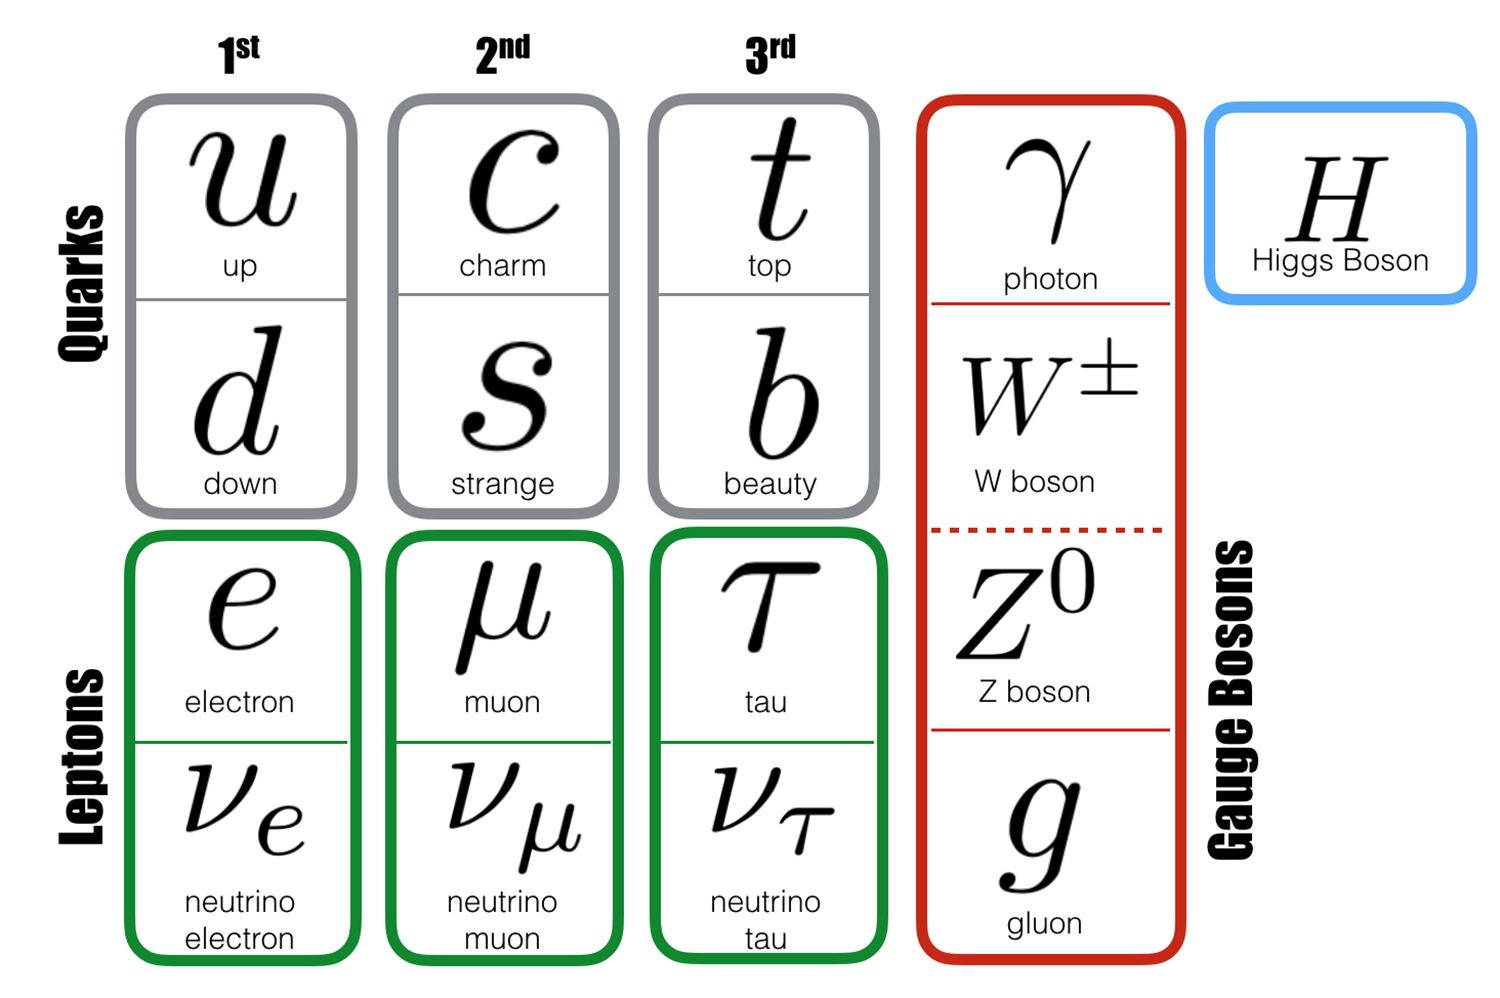
\includegraphics[width=\textwidth]{Bilder/SM.png}
	\caption[Standard Model]{The particles of the Standard Model include three families of quarks and leptons, four gauge bosons and the Higgs boson. The beige background indicates which bosons interact with which fermions. \cite{SMFigure}}
	\label{fig:SM}
\end{figure}



Figure \ref{fig:SM} shows the fundamental particles of the standard model. It includes three families of quarks and leptons so-called \textit{fermions}, four \textit{gauge bosons} and the Higgs \textit{boson}. Fermions and bosons differ by the spin. Spin is a degree of freedom, which had to be introduced to conserve the angular momentum in the Dirac equation. The matter forming fermions have a half-integral spin (in units of the reduced Planck constant $\hbar$) and the bosons (the exchange particles as well as the Higgs particle) have an integer spin. The fermion family can be sectioned into two families. The \text{quark} and the lepton family. 
The quark familiy consist of up- (u), down- (d), strange- (s), charm- (c), bottom- (b) and top- (t) quark. Quarks have fractional electric charge values. u-, c- and t-quark have an electric charge of $\nicefrac{2}{3} \,e$ and d-, s- and b-quark have an electric charge of $-\nicefrac{1}{3} \,e$. As indicated in figure \ref{fig:SM} by the beige background, quarks can interact with all four gauge bosons.
The lepton family is made of the electron ($e$), the muon ($\mu$) and the tau ($\tau$) and their corresponding neutrinos $\nu_e,\nu_{\mu} \textrm{ and } \nu_{\tau}$. The neutrinos can only interact via the weak exchange particles ($W^{\pm}$ and $Z$ bosons). Since the electrons, muons and taus are charged, they can also interact with photons.

All fermions also have so-called \textit{antiparticles}. Antiparticles have the same mass as their corresponding particle but they have opposite charge. For example, the antiparticle of the electron is the positron. Both have the same mass and the same spin but the electron has an electric charge of $-1\,e$ and the positron has an electric charge of $+1\,e$. When a particle collides with its antiparticle annihilation can occur. In an annihilation process the incoming particles are destroyed to produce other particles. The final particles carry the same energy and momentum as the initial particles.\\


All visible matter in the universe is made of fermions from the first family. For example, atoms consist of protons and neutrons, each of which is a combination of up and down quarks. In the electron shell of an atom the eponymous electrons are located. Pauli proposed the neutrino in the 1930 to explain the energy spectrum of electrons in $\beta$-decays. Since neutrinos are only weak interacting particles, they were not observed until 1956.\cite{REINES19941} With increasing energy, the second and third family have been gradually discovered, first from cosmic ray experiments in the 1930s up to the discovery of the Higgs boson at the Large Hadron Collider (LHC) at Cern in 2012. Parallel to the experimental discoveries, the theory also evolved, partially explaining the results and in part motivating new experiments through predictions.


\section{Physics Beyond The Standard Model}

Despite the success of the standard model as an effective theory, it fails answering a lot of open questions. As already mentioned, the standard model only includes three out of four fundamental forces. It does not include gravity, therefore, the standard model is not valid at energy scales approaching the Planck energy $E_P \approx 1.22\cdot 10^{19}\,\textrm{GeV} $.\cite{sivaram2007special} It is also unable to explain dark matter, dark energy and the matter/antimatter asymmetry in the universe which is directly linked to charged-parity violation.\cite{HAMBYE2012193}

\section{Bhabha Scattering}
\label{sec:Bhabha}

In this section, we want to briefly discuss Bhabha scattering. We will start with the physics of Bhabha scattering and then discuss the Bhabha kinematics at Belle II.
 
\subsection{Bhabha Process}
 \label{sec:BhabhaProcess}
 Bhabha scattering is a quantum electromechanical process between an electron and a positron. It is named after the Indian  physicist H. Bhabha who first derived the electron-positron scattering cross section in 1935.\cite{Bhabha}
 
 Bhabha scattering contains two different processes. Both have in common that there is an electron and positron in the initial and final state. Figure \ref{fig:feynman} shows the Feynman diagrams for both Bhabha processes. The time passes from the left to the right side. In the left process, the initial electron and positron annihilate to form a virtual photon $\gamma^\ast$. This virtual photon then decays into an electron and a positron. The right Feynman diagram describes a classic electrodynamic scattering process. Here the incoming electron and positron are scattering by the interaction with a virtual photon. In contrast to the right diagram, the left diagram can only be explained by quantum field theory, due to the creation and destruction of particles.
 

\tikzset{
	photon/.style={decorate, decoration={snake}, draw=red},
	particle/.style={draw=blue, postaction={decorate},
		decoration={markings,mark=at position .5 with {\arrow[draw=blue]{>}}}},
	antiparticle/.style={draw=blue, postaction={decorate},
		decoration={markings,mark=at position .5 with {\arrow[draw=blue]{<}}}},
	gluon/.style={decorate, draw=black,
		decoration={coil,amplitude=4pt, segment length=5pt}}
}





\begin{figure}[h!]
		\centering

\begin{minipage}{.5\textwidth}

\begin{tikzpicture}[
thick,
% Set the overall layout of the tree
level/.style={level distance=1.5cm},
level 2/.style={sibling distance=2.6cm},
level 3/.style={sibling distance=2cm}
]
\coordinate
child[grow=left]{
	child {
		node {$e^+$}
		% The 'edge from parent' is actually not needed because it is
		% implicitly added.
		edge from parent [particle]
	}
	child {
		node {$e^-$}
		edge from parent [antiparticle]
	}
	edge from parent [photon] node [above=3pt] {$\gamma^\ast$}
}
% I have to insert a dummy child to get the tree to grow
% correctly to the right.
child[grow=right, level distance=0pt] {
	child {
	node {$e^-$}
	% The 'edge from parent' is actually not needed because it is
	% implicitly added.
	edge from parent [particle]
}
child {
	node {$e^+$}
	edge from parent [antiparticle]
}
edge from parent [photon] 
}
	
;
\end{tikzpicture}


\begin{tikzpicture}
\begin{scope},scale=1]
\draw[->,thick]
(-4,-1.8) -- (1,-1.8)
;
\draw
(-1.5,-1.8) node[anchor=south]{$t$};
\end{scope}


\end{tikzpicture}


\end{minipage}
\begin{minipage}{.2\textwidth}

\begin{tikzpicture}[
thick,
% Set the overall layout of the tree
level/.style={level distance=1.5cm},
level 2/.style={sibling distance=2.6cm},
level 3/.style={sibling distance=2cm}
]
\coordinate
child[grow=up]{
	child {
		node {$e^+$}
		% The 'edge from parent' is actually not needed because it is
		% implicitly added.
		edge from parent [antiparticle]
	}
	child {
		node {$e^+$}
		edge from parent [particle]
	}
	edge from parent [photon] node [right=3pt] {$\gamma^\ast$}
}
% I have to insert a dummy child to get the tree to grow
% correctly to the right.
child[grow=down, level distance=0pt] {
	child {
		node {$e^-$}
		% The 'edge from parent' is actually not needed because it is
		% implicitly added.
		edge from parent [antiparticle]
	}
	child {
		node {$e^-$}
		edge from parent [particle]
	}
	edge from parent [photon] 
}

;
\end{tikzpicture}

\begin{tikzpicture}
\begin{scope},scale=1]
\draw[->,thick]
(-4,0) -- (-0.8,0)
;
\draw
(-2.4,0) node[anchor=south]{$t$};
\end{scope}


\end{tikzpicture}


\end{minipage}






\caption[Bhabha Feynman Diagrams]{The two Bhabha process Feynman digrams. The left diagram describes the annihilation and pair production process, while the right diagram describes a classic electromagnetic scattering process.}
\label{fig:feynman}


\end{figure}


\subsection{Differential Cross Section Of Bhabha Processes}
\label{sec:cross-section}

The cross section describes the probability that two particle will interact with each other when they collide. If this collision creates secondary radiation, then the intensity distribution over the spatial direction $\Omega$ is described by the differential cross section $\nicefrac{\textrm{d}\sigma}{\textrm{d}\Omega}$.

The differential cross section for the electron\footnote{The electrons are moving along the x-axis. The positrons are moving in the opposite direction} in a Bhabha process is given by equation \ref{eq:bhabhaCross}. 

\begin{equation}
	\bigg(\frac{\textrm{d}\sigma}{\textrm{d}\Omega} \bigg)_{\textrm{cms}} = \frac{e^4}{32\pi^2 E^2}
	\bigg(
	\frac{1+\textrm{cos}^2(\theta)}{2} +
 \frac{1+\textrm{cos}^4(\nicefrac{\theta}{2})}{\textrm{sin}^4(\nicefrac{\theta}{2})} - \frac{2\textrm{cos}^4(\nicefrac{\theta}{2})}{\textrm{sin}^2(\nicefrac{\theta}{2})}   \bigg)
 \label{eq:bhabhaCross}
\end{equation}



\begin{figure}[h!]
	\centering
	\begin{minipage}[b]{0.47\linewidth}
		\centering
		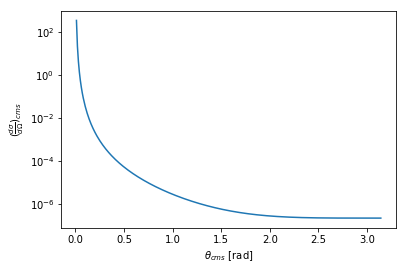
\includegraphics[width=\textwidth]{Bilder/dsdO}
	\end{minipage}
	\hspace{0.5cm}
	\begin{minipage}[b]{0.47\linewidth}
		\centering
		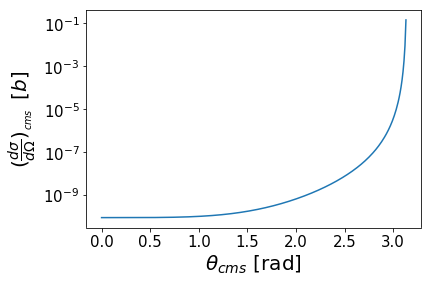
\includegraphics[width=\textwidth]{Bilder/dsdO1}
	\end{minipage}
	\caption[Differential Cross Section For Electrons And Positrons In Bhabha Events]{Differential cross-section for Bhabha events. Left: The Cross-section for electrons is shown and on the left for positrons.
	
These plots were created with python3.}
	\label{fig:CrossSectionElPos}
	\end{figure}

In figure \ref{fig:CrossSectionElPos} on the left, the differential cross section for electrons is plotted. Since, most incoming particles are only very slightly deflected, the cross section is very high for small angels and gets smaller with increasing angle. Equation \ref{eq:bhabhaCross} is also true for positrons but since they are moving in the opposite direction,therefore, $\theta$ has to be replaced by $\pi - \theta$ in equation \ref{eq:bhabhaCross}. This result is plotted in figure \ref{fig:CrossSectionElPos} on the right.




\begin{figure}[h!]
	\centering
	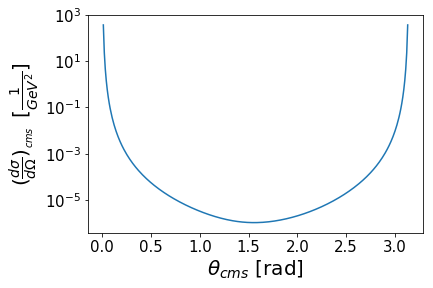
\includegraphics[width=10cm]{Bilder/dsdOb}
	\caption[Differential Cross Section For Bhabha Events]{This figure shows to differential cross section for Bhabha events. 
		
		This plot was created with python3.}
	\label{fig:CrossSectionBoth}
\end{figure}

To get to differential cross section for Bhabha events, one has to add the differential cross section of electrons and positrons. This is shown in figure \ref{fig:CrossSectionBoth}. As you can see, most of the outgoing particles will have a very small or very large $\theta$ angle.


\subsection{Bhabha Kinematics At Belle II}
\label{sec:Kinematics}

At Belle II the electron and the positron beams have different energies. Also, they are hitting each other under an angle. Therefore, it is interesting to look at the Bhabha kinematics in the lab system of Belle II.

\begin{figure}[h!]
	\centering
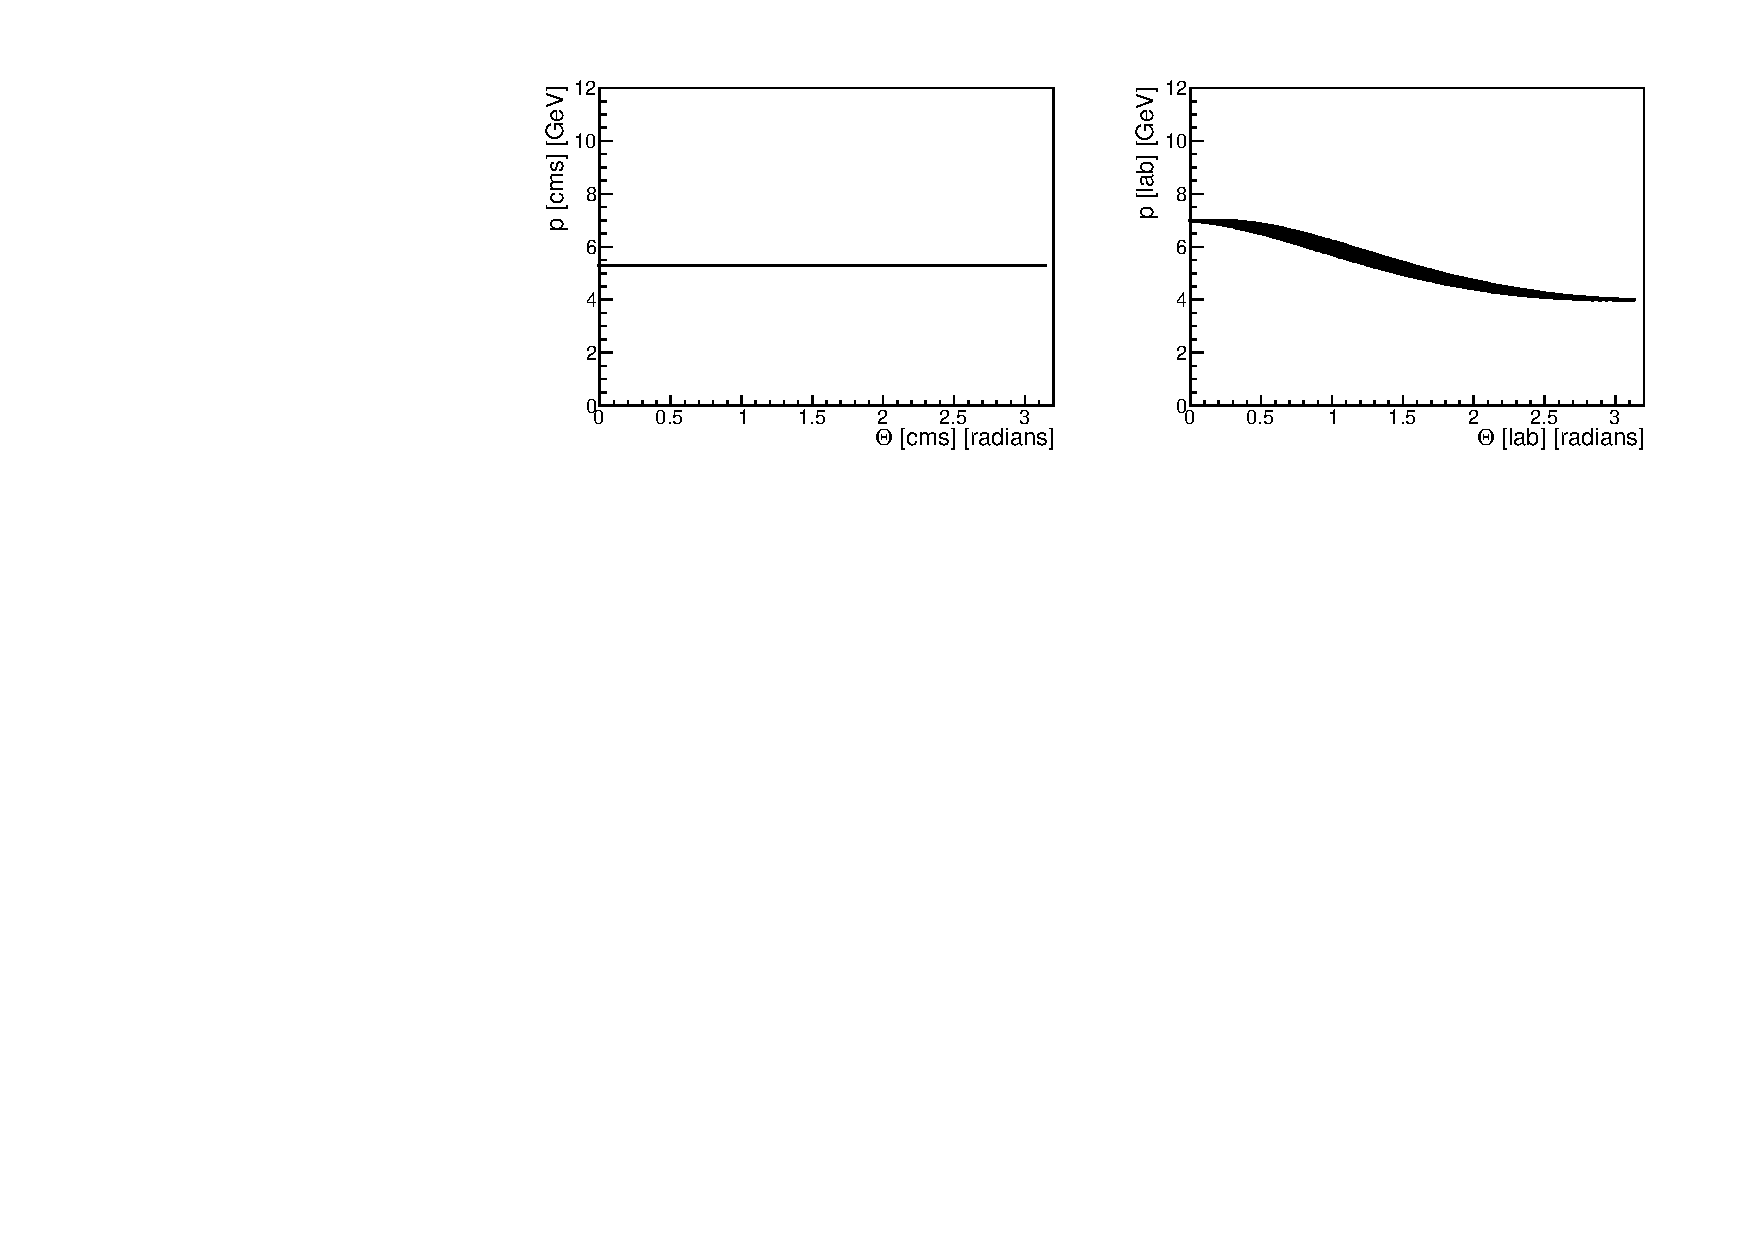
\includegraphics[width=\textwidth]{Bilder/CThetaP}
	\caption[$\theta$-Momentum-Distribution In The CMS And LAB Frame]{Bhabha scattering in different frames. In the CMS the particle has the same Belle II energy in every $\theta$-direction. Left: The $\theta$-Energy-distribution in the CMS frame is shown. Right: The $\theta$-Energy-distribution in the lab frame is shown.}
	\label{fig:Belle IIMomentum}
	
\end{figure}

Figure \ref{fig:Belle IIMomentum} on the left, you can see  the momentum of the Bhabha particles as a function of the $\theta$ angle in the center-of-mass frame. Since the incoming electron and the positron have the same mass and they are hitting each other with the same energy, the outgoing particles always have the same momentum independent of the $\theta$ angle in the center of mass frame. In the right plot, you can see the momentum distribution after the boost in the lab system. For small $\theta$ angles a higher momentum of the outgoing particles is expected compared to high $\theta$ angles. The fanning of the distribution is cased by the fact that the beams are hitting each other under an angle at Belle II. Also, due to the fanning, we expect a range of energies at a fixed $\theta$ angle.



\begin{figure}[h!]
	\centering
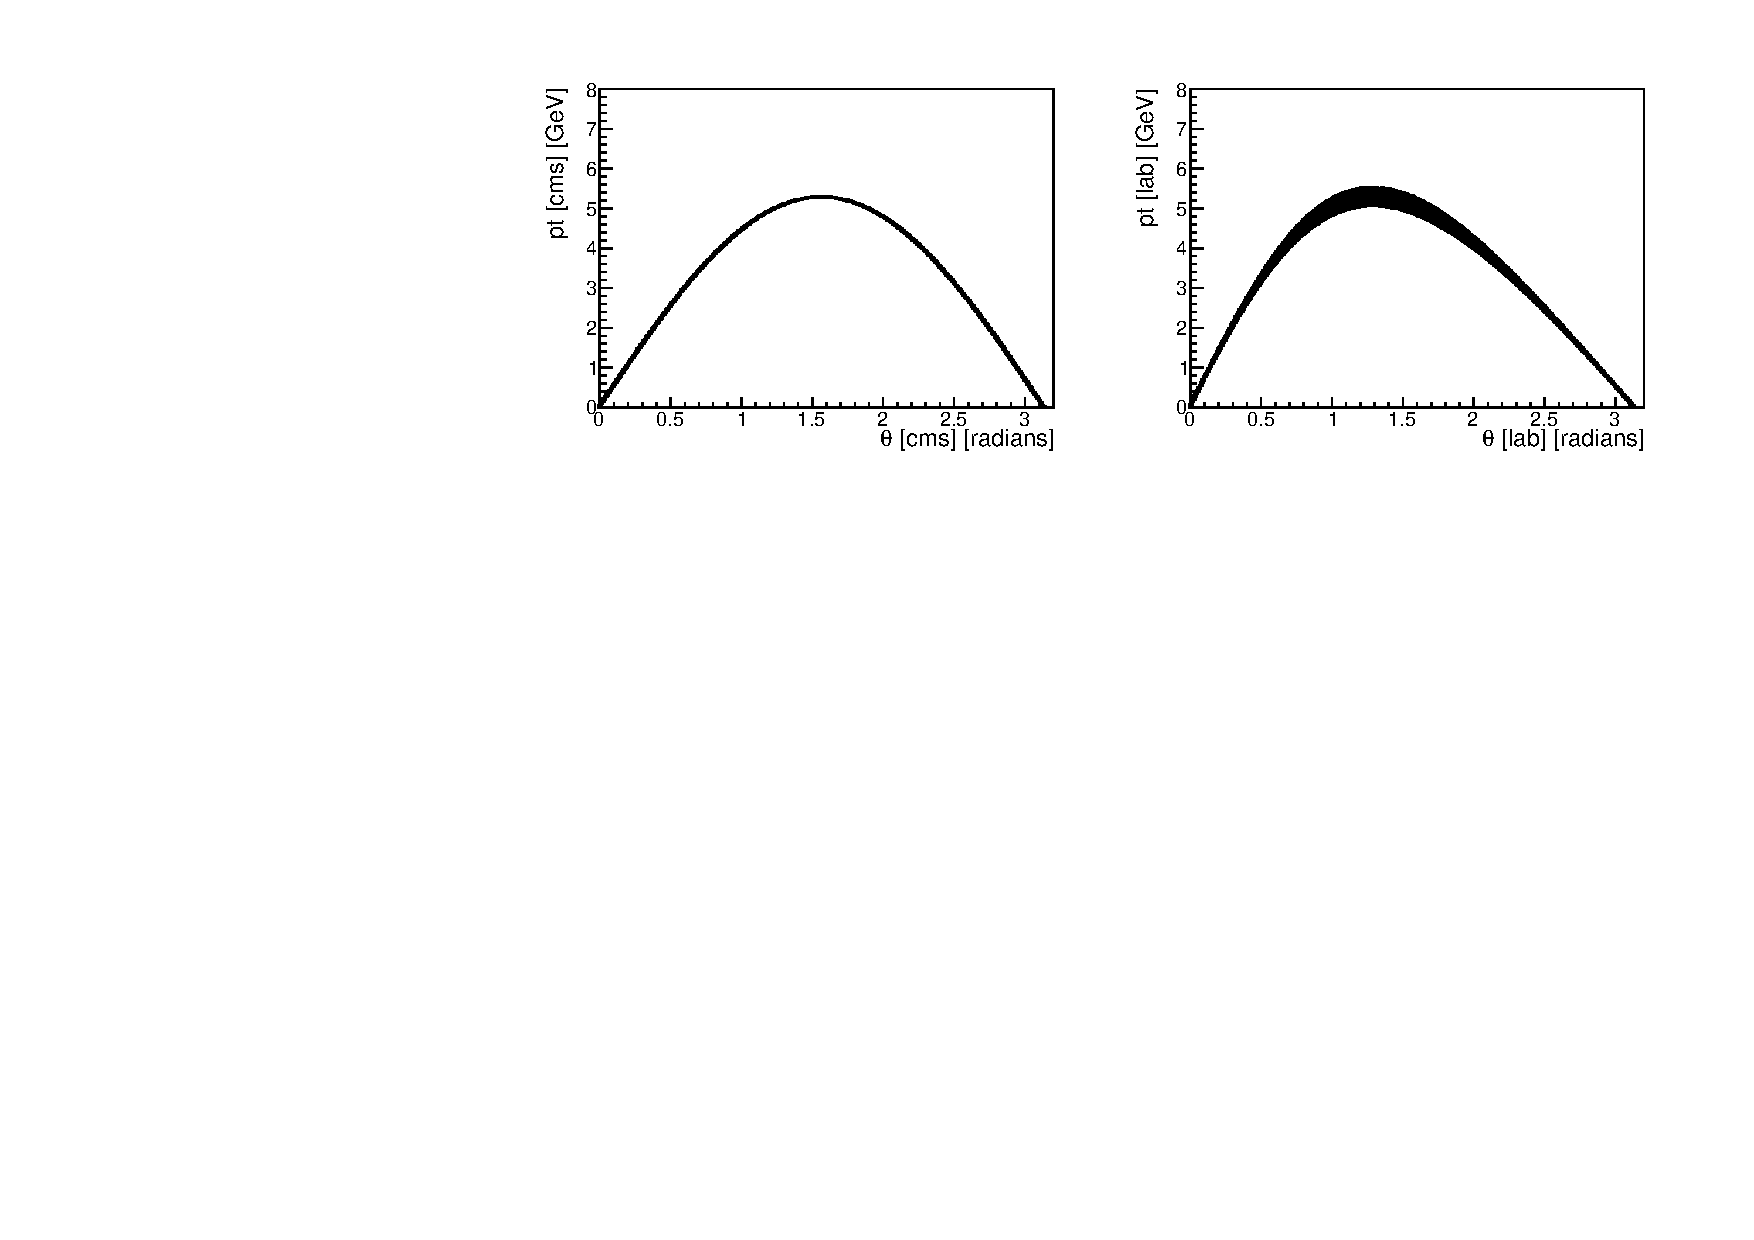
\includegraphics[width=\textwidth]{Bilder/CptTheta}
	\caption[$\theta$-Transverse Momentum-Distribution In The CMS And LAB Frame]{The transverse momentum of the outgoing Bhabha particles in different frames. Left: transverse momentum in the center-of-mass frame. The highest transverse momentum is expected at an $\theta$ angle of $\nicefrac{\pi}{2}$.  Right: The transverse momentum in the lab frame. The highest transverse momentum is shifted a bit to smaller values of $\theta$.}
	\label{fig:Belle IItMomentum}
\end{figure}


Figure \ref{fig:Belle IItMomentum} shows the transverse momentum as a function of $\theta$ for the outgoing Bhabha particles at Belle II. The left plot shows the distribution in the center-of-mass frame, while the right plots shows it for the lab frame. In both frames, we expect the highest transverse momentum at an $\theta$ angle of about $\nicefrac{\pi}{2}$.



\begin{figure}[h!]
	\centering
	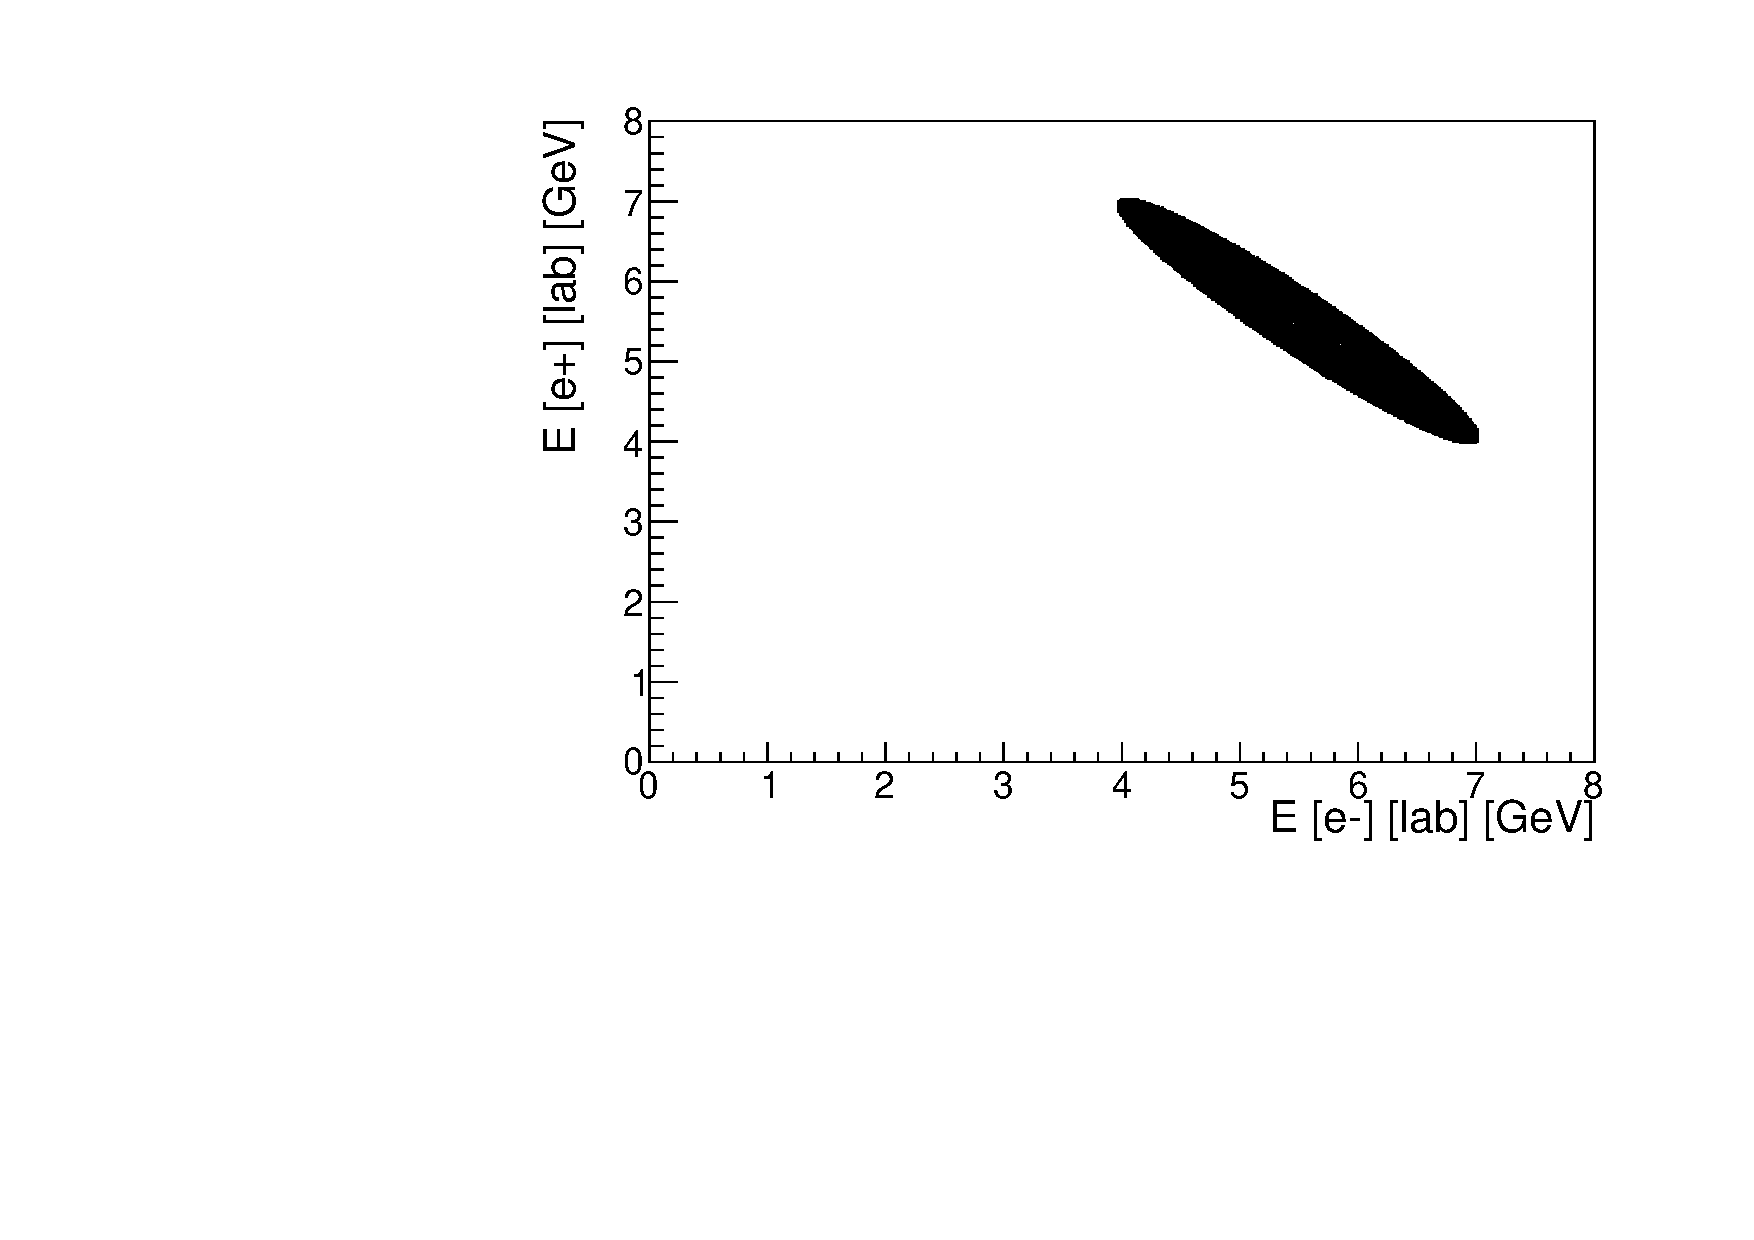
\includegraphics[width=10cm]{Bilder/ee}
	\caption[Energies Of The Outgoing Particle In The LAB Frame]{The energy of the two outgoing Bhabha particles in the lab frame at Belle II.}
	\label{fig:EvsE}
\end{figure}

In figure \ref{fig:EvsE} the energy of the outgoing Bhabha particles in the lab frame at Belle II are plotted against each other. As you can see, if for example the electron has an energy of $7\,\textrm{GeV}$ than the positron will have an energy of just about $4\,\textrm{GeV}$ and vice versa.










%_______________________________________________________________________________
\chapter{Experimental Setup At SuperKEKB}
\label{sec:SetupKEK}

\lettrine{S}{uperKEKB} is a two-ring, asymmetric\footnote{asymmetric means that there is an energy difference between the two colliding beams}, electron positron accelerator, which is located at KEK (\textit{High Energy Accelerator Research Organization}) in Tsukuba, Japan. 
The electron beam has an energy of $7\,\textnormal{GeV}$ and the positron beam has an energy of $4\,\textnormal{GeV}$. These beams collide with a center-of-momentum energy of about $10.58\,\textnormal{GeV}$, which is close to the mass of the $\Upsilon(4\textnormal{S})$ resonance. Therefore SuperKEKB is a so-called \textit{B-factory}. The decay products are then detected by the Belle II detector to study the properties of these B mesons with high precision. In early 2018 Belle II started taking data. One goal of Belle II is to study CP-Violation with respect to new physics.\cite{B2B}

\section{KEKB And SuperKEKB}
\label{sec:KEK}
This section will only provide a rough overview of the SuperKEKB accelerator since the focus of this work is on the analysis. 

SuperKEKB is an upgrade of the KEKB accelerator. KEKB was also an asymmetric electron positron accelerator in the period from 1998 to 2010, but the energies were different compared to SuperKEKB. At KEKB the electrons were accelerated to an energy of $8\,\textrm{GeV}$ and the positrons to an energy of $3.5\,\textrm{GeV}$. KEKB was also a B-factory and the reaction products were then detected in the Belle detector. In 2009 KEKB achieved an instantaneous luminosity of $\mathcal{L} = 2.11 \cdot 10^{34}\,\textrm{cm}^{-1}\textrm{s}^{-1}$. This was the world record at that time. KEKB was discontinued after more than 10 years, to be upgraded to SuperKEKB.\cite{PTEP}


\begin{figure}[h!]
\begin{center}
	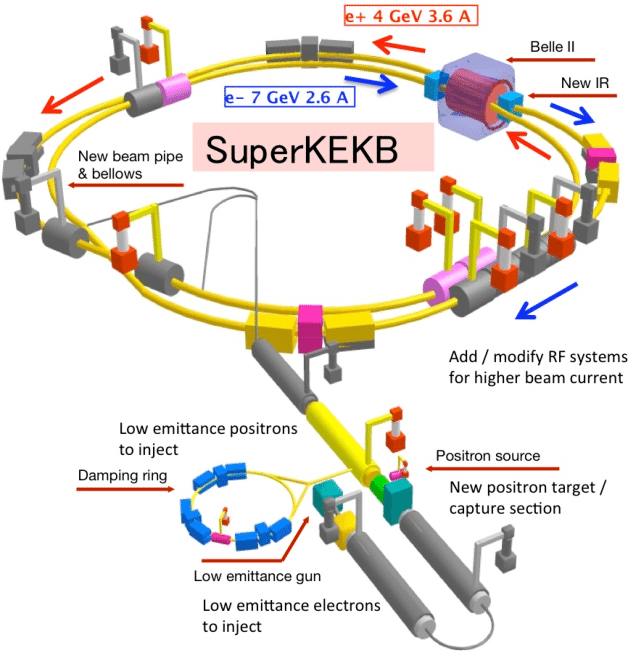
\includegraphics[width=\textwidth]{Bilder/SuperKEKB.png}
	
	\caption[SuperKEKB Collider]{The SuperKEKB collider.\cite{SKEKAcc}}
	\label{fig:SuperKEKB}
\end{center}
\end{figure}






In figure \ref{fig:SuperKEKB} you can see the schematic layout of the SuperKEKB accelerator. The electrons are start at the Low emittance gun. They are then accelerated in the \textit{J}-shaped linear particle accelerator (linac). Due to lack of space, the linac has to have this special form.\cite{KEKBJArc} After the curve and a second acceleration stage the electrons hit the positron production target, where the positrons are created. After this target, there are more acceleration stages, before the two beam are then injected into their independent storage rings. The electrons are stored in the high-energy ring (HER) and the positrons are stored in the low-energy ring (LER). Each of these rings has a circumference of about $3\,\textrm{km}$. Both beams collide at the interaction region (IR). The products of the collisions are then detected by the Belle II detector, an upgraded version of the Belle detector.\cite{B2B} (See section \ref{sec:Belle II})

SuperKEKB uses a smaller asymmetry in the beam energies compared to KEKB. This allows the usage for higher beam currents and better focusing magnets. This can then result into a higher luminosity. The goal is to achieve a 40 times higher luminosity with SuperKEKB compared to KEKB.
An integrated luminosity of $50\,\textrm{ab}^{-1}$ will be achieved by 2025.\cite{B2B}

The instantaneous luminosity $\mathcal{L}$ specifies the performance of the collider. Knowing $\mathcal{L} $ and the cross section $\sigma$ one can calculate the events per second for a process by the following formula.
\begin{equation}
\frac{\textrm{d}N}{\textrm{d}t} = \mathcal{L} \cdot \sigma
\end{equation} 

To increase the event rate one has to increase the instantaneous luminosity since $\sigma$ is given by the processes. The instantaneous luminosity can be calculate by the following equation.
\begin{equation}
	\mathcal{L} = \frac{N_{e^-}N_{e^+}f_c}{4\pi \sigma_x \sigma_y} \cdot S
	\label{eq:Lumi}
\end{equation}

One has to assume that both beams have a Gaussian profile of horizontal and vertical size $\sigma_x$ and $\sigma_y$. In equation \ref{eq:Lumi} $N_{e^-}$ is the number of particles in an electron bunch and $N_{e^+}$ is the number of particles in a positron bunch. $f_c$ is the average crossing rate, which can be calculated by $f_c = n \cdot f_r$. Where $n$ is the number of bunches and $f_r$ is the revolution frequency. $S$ is a reduction factor which takes geometrical effects linked to the finite cross section and bunch length into account.\cite{herr2006concept} 
SuperKEKB increased the luminosity by a factor of two compared to KEKB by increasing the number of bunches and the number of particles per bunch.
 


\begin{figure}[h!]
	\centering
	\begin{minipage}[b]{0.45\linewidth}
		\centering
		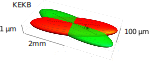
\includegraphics[width=\textwidth]{Bilder/BeamBelle}
	\end{minipage}
	\hspace{0.5cm}
	\begin{minipage}[b]{0.45\linewidth}
		\centering
		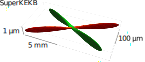
\includegraphics[width=\textwidth]{Bilder/SuperKEKBBeam}
	\end{minipage}
		\caption[Sketch Of The Beam Crossing For KEKB And SuperKEKB]{Sketch of the beam crossing at KEKB (left) and SuperKEKB (right). At KEKB the size of the interaction region was about $10\,\textrm{mm}$. At SuperKEKB it is about $0.5\,\textrm{mm}$.\cite{Beamsize} This figure was edited in order to make the axis more readable.}
	\label{fig:beamsize}

\end{figure}







Also, the size of the interaction region at SuperKEKB is just one twentieth of what it was at KEKB, resulting in a vertical beam size of $\sigma \approx 50\,\textrm{nm} $. This can be seen in figure \ref{fig:beamsize}. This decrease in beam size along with the increase in the beam currents  results in a overall 40-fold increase in luminosity.  \cite{B2TR} \cite{B2B}



\section{The Belle II Detector}
\label{sec:Belle II}

The Belle II detector is an upgraded version of the Belle detector which was a solid-angle magnetic spectrometer located at the interaction region of KEK. In figure \ref{fig:Belle2} a sketch of the Belle II detector is shown. The detector contains of a variety of sub-detectors, each fulfilling a specific purpose.
 
\begin{figure}[h!]
	\centering
	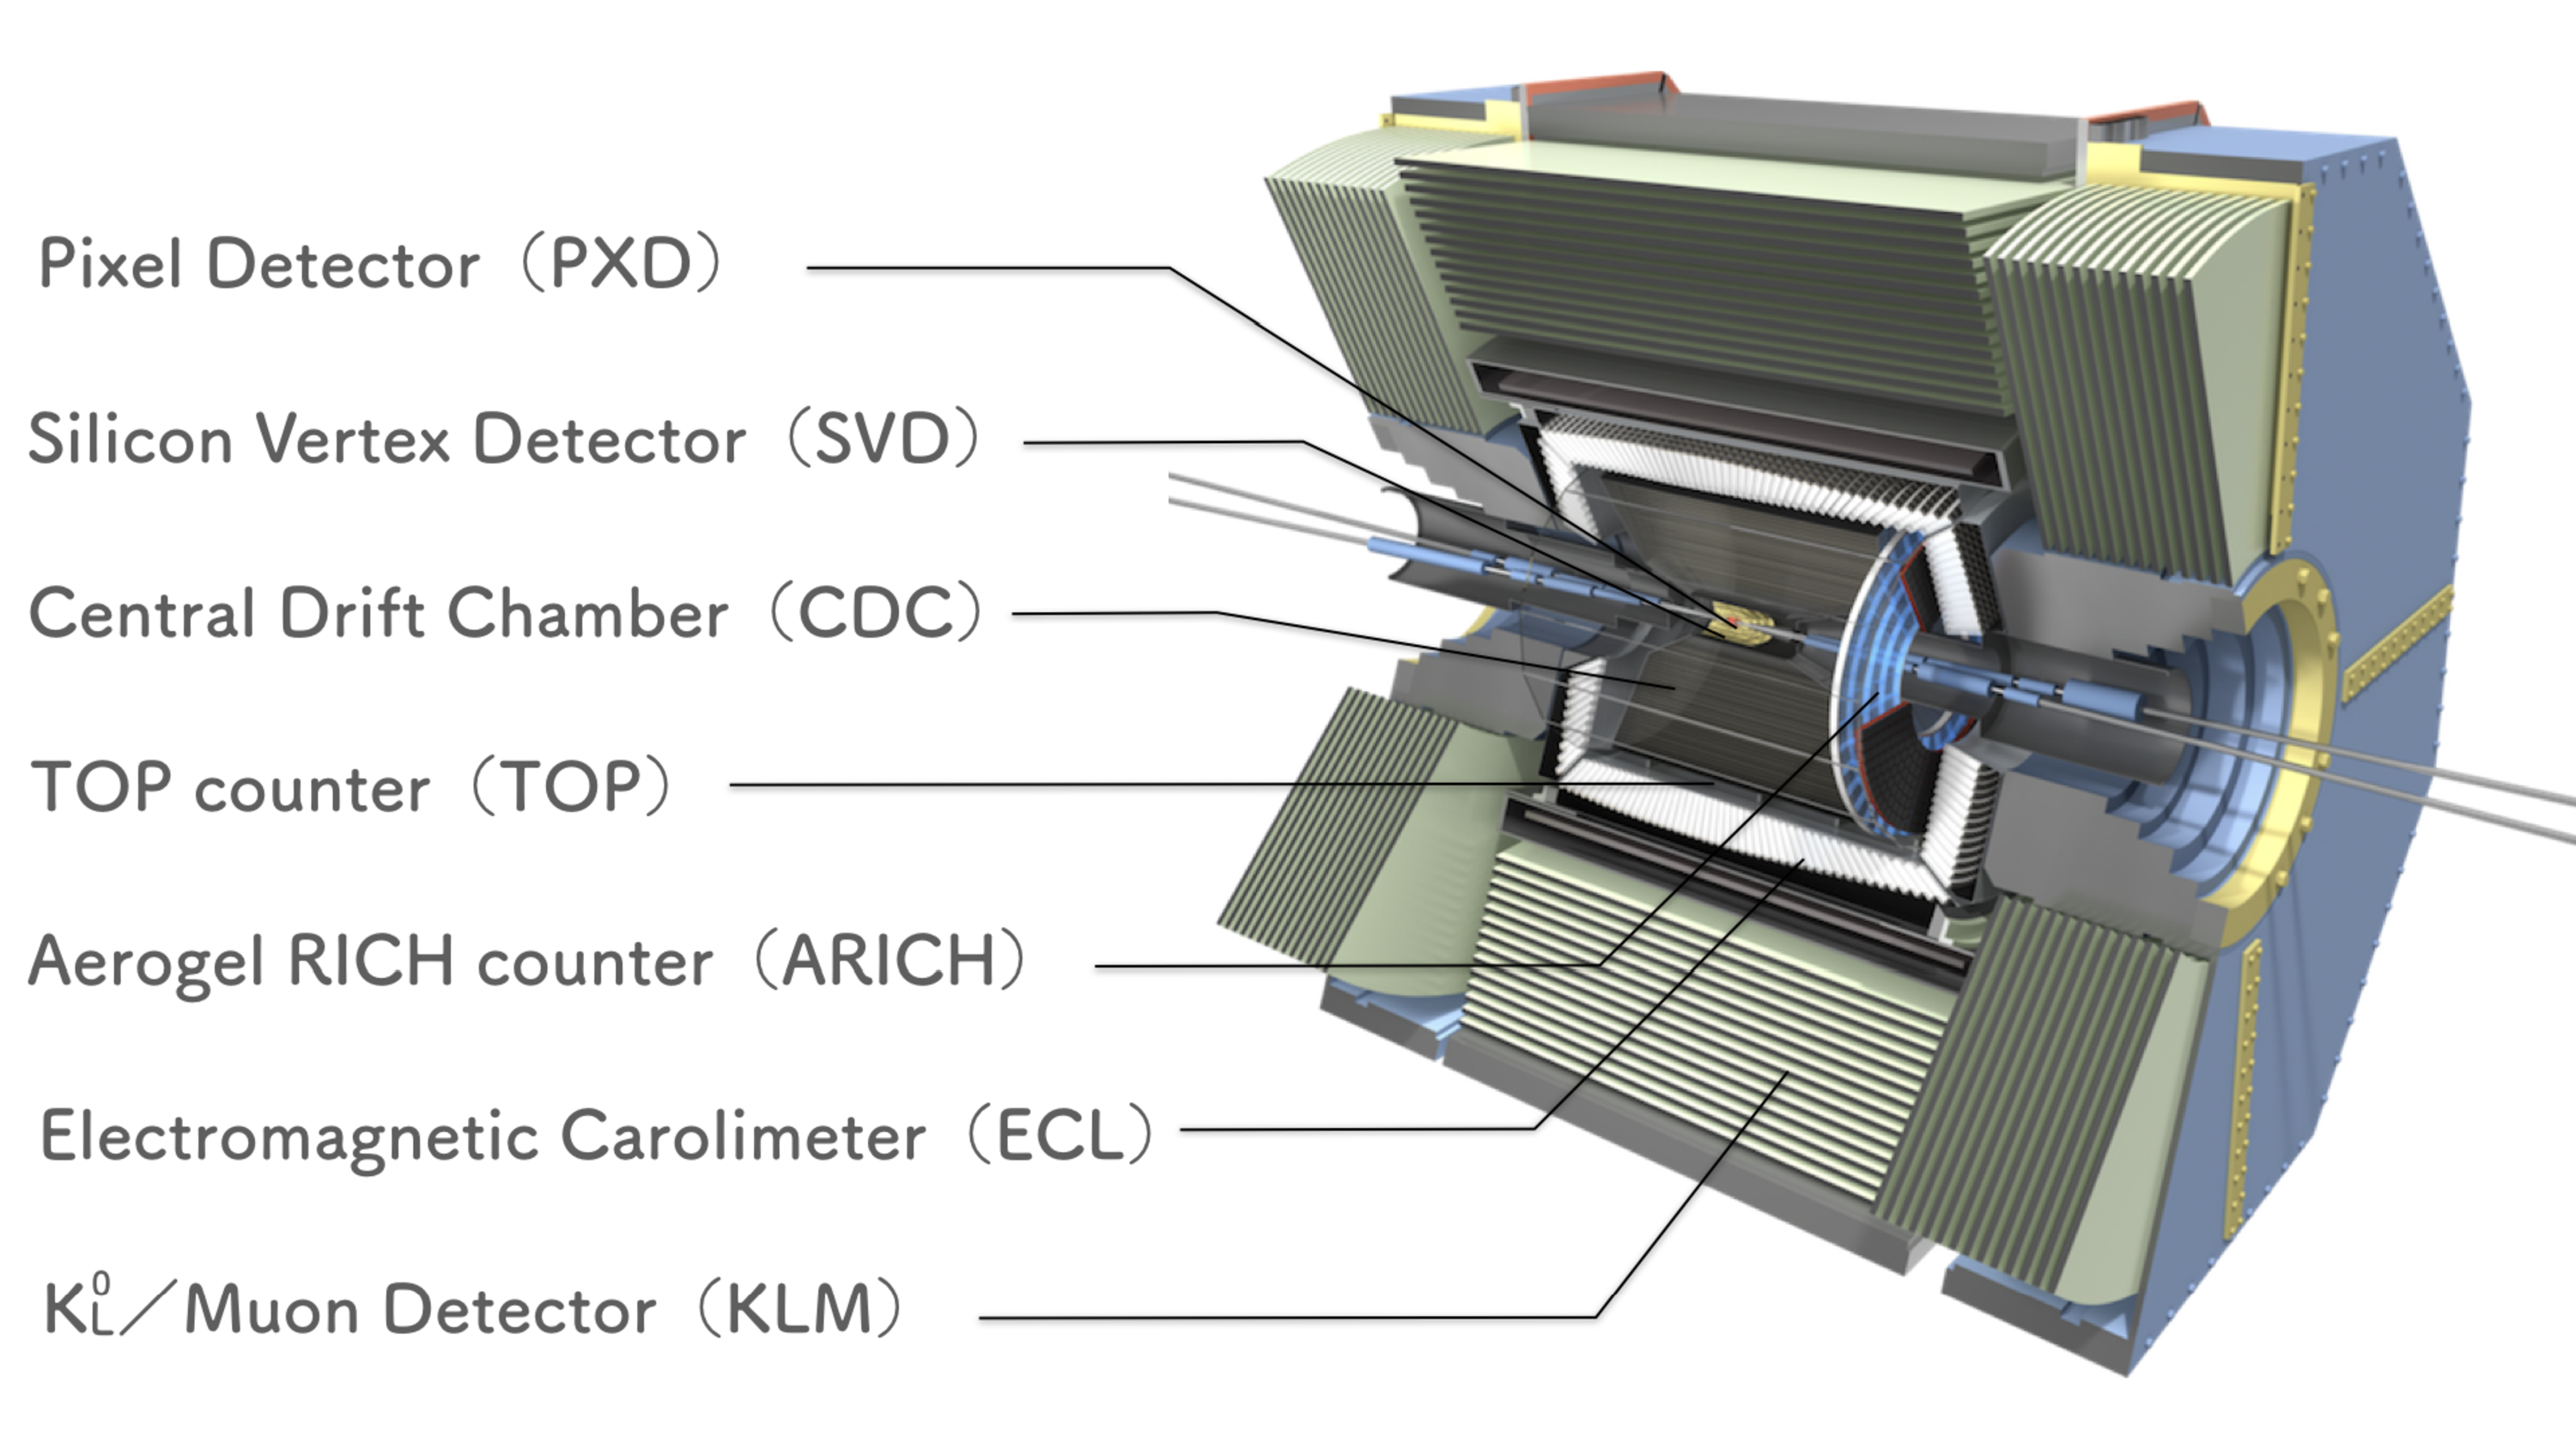
\includegraphics[width=\textwidth]{Bilder/Belle2.pdf}
	
	\caption[Belle II Detector]{Schematic view of the Belle II detector. The different detector elements are labeled. Also the beam pipes for the electrons and positrons with their corresponding energies are shown. \cite{BDetector} This figure was modified in order to make the text more readable.}
	\label{fig:Belle2}
\end{figure}

 In the innermost of the detector, three tracking sub-detectors are located, surrounding the IR. These sub-detectors are in a axial magnetic field of $1.5\,\textrm{T}$, provided by a solenoid, to be able to reconstruct the tracks of charged particles. 
 
 The vertex detectors, consisting of the silicon vertex detector (SVD), an upgraded version of the SVD used in Belle, and the pixel detector (PXD), a new detector designed for Belle II, are used to measure the momenta of charged particles and to reconstruct decay vertices and particles with a momentum too low to reach the central drift chamber (CDC).

The CDC also already existed in the Belle detector and has been upgraded for Belle II. The CDC scans the trajectories of charged particles. From these trajectories the charge, momentum and energy loss can be determined by ionization. 

These three innermost tracking detectors are surrounded by a barrel. The time-of-propagation (TOP) detector, which also got an upgrade for Belle II, surrounds the inner detectors parallel to the beam-pipes. The TOP detector, as the name suggests, measures the flight-time of charged particles. Knowing the flight-time and the momentum of the charged particles, it is possible to conclude their mass and to identify them. The forward end-cap of the barrel is closed with an Aerogel Ring-Imaging Cerenkov detector (ARICH) which also identifies charged particles.

The next outer detector is the electromagnetic calorimeter (ECL). It surrounds all the previously mentioned detectors, and was already installed in Belle. The ECL is able to measure the energy of electromagnetically interacting particles, especially photons and electrons.

The task of the outermost detector the $K_L^0$ and muon detector (KLM) is to identify $K_L^0$ and muons. The KLM also got upgraded for Belle II. \cite{B2B} 

\section{Coordinate System}

For clarification, the coordinate system of Belle II will be described in this section, before the detectors are explained in more detail.

\begin{figure}[h!]
	\begin{center}
		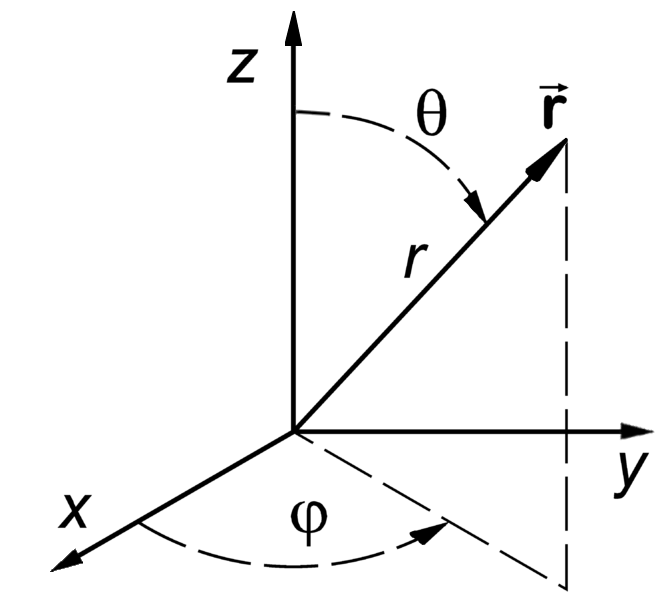
\includegraphics[width=5cm]{Bilder/coordinate.png}
	\end{center}
	\caption[Coordinate System Of Belle II]{A sketch of the coordinate system of Belle II. The original figure was modified to make the coordinate system more visible. \cite{TrackReconstruction}}
	\label{fig:CoordinateSysytem}
\end{figure}

A sketch of the coordinate system is shown in figure \ref{fig:CoordinateSysytem}. The origin of the coordinate system corresponds to the interaction region. For the Cartesian coordinate system: The $z$-axis points in the direction of the magnetic field. This is also the so-called forward direction. The $y$-axis points up to the upper part of the detector. The $x$-axis points along the radial direction of the accelerator. The electrons are moving roughly along the positive $z$ axis, while the positrons are moving in the opposite direction. In figure \ref{fig:CoordinateSysytem} also the spherical coordinate system is shown. Here $\theta$ corresponds to the polar angle and $\phi$ to the azimuthal angle.\cite{DevelopVertex}

\section{Vertex detector}
\label{sec:vertexDet}

The vertex detectors (VXD) are able to make precise measurements of the tracks of particles close to the interaction region. This allows the reconstruction of decay-vertices of long-lived particles. For this it is very important to determine the distance and the spatial resolution of the first measured hit, and the effect of multiple scattering.


\begin{figure}[h!]
	\begin{center}
		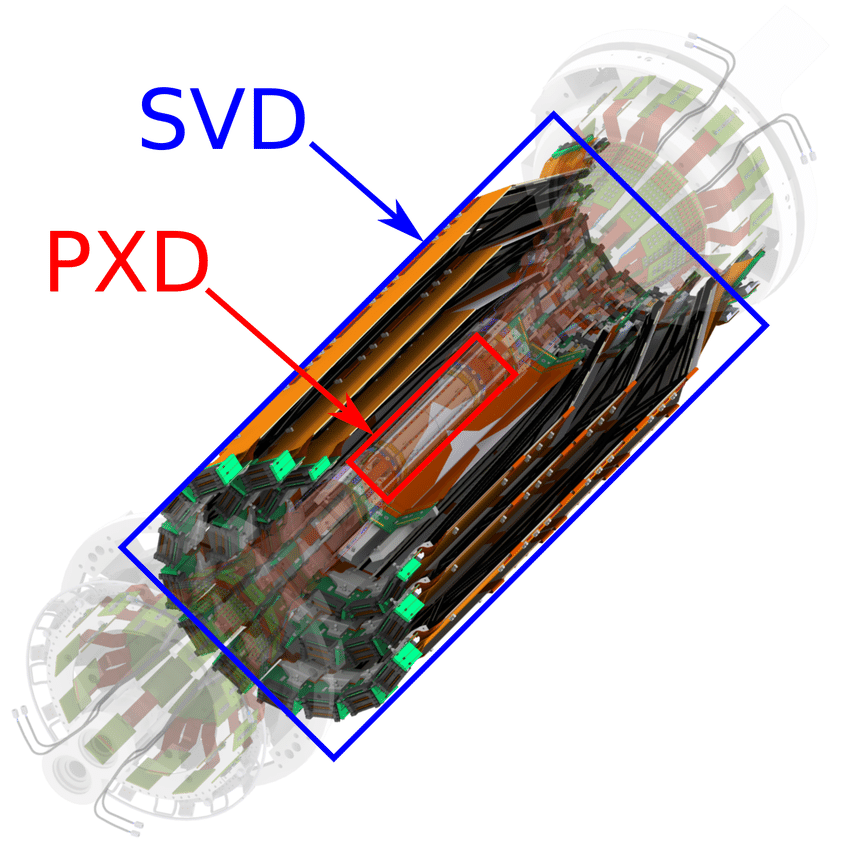
\includegraphics[width=10.5cm]{Bilder/PXD_SVD}
	\end{center}
\caption[Vertex Detector]{Sketch of the vertex detectors. The vertex detector itself consists of two sub-detectors. The PXD is surrounded by the SVD. \cite{OnlineDataReduction} }
\label{fig:VertexDet}
\end{figure}

The VXD consists of the pixel vertex detector and the silicon vertex detector, both can be seen in figure \ref{fig:VertexDet}. These two detectors complement each other.


\subsection{Pixel Vertex Detector}
\label{sec:Pixel}
The purpose of the PXD is to reconstruct the spatial position of the decay vertices of $B$, $D$ and $\tau$.
The PXD is based on Depleted P-channel Field-Effect Transistor (DePFET) technology. This technology allows the sensors of the PXD to be very thin ($\sim 50\,\mu\textrm{m}$).

\begin{figure}[h!]
	\begin{center}
		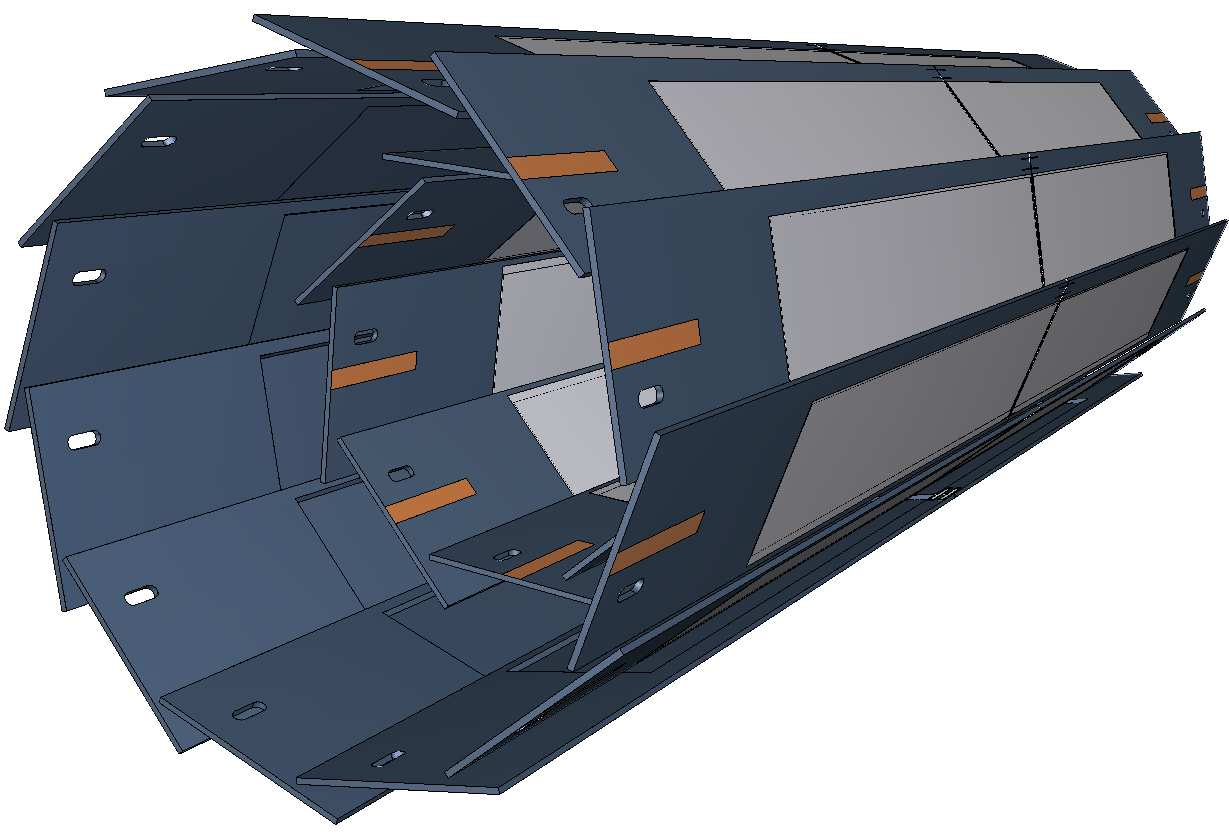
\includegraphics[width=12cm]{Bilder/pixel}
	\end{center}
	\caption[Pixel Detector]{Sketch of the complete PXD \cite{B2TR}}
	\label{fig:pxd}
\end{figure}

As you can see in figure \ref{fig:pxd}, the PXD consists of two layers of sensors. The inner layer is made out of eight planar sensors (ladder), each has a width of $15\,\textrm{mm}$ and an effective length of $90\,\textrm{mm}$. This layer has a radius of $14\,\textrm{mm}$. The second layer consists of 12 planar sensors. These sensors also have a width of $15\,\textrm{mm}$, but a length of $123\,\textrm{mm}$. The radius for the second layer is $22\,\textrm{mm}$. The PXD provides a spatial resolution of about $1.2\,\mu\textrm{m}$.\cite{B2TR}

Due to the vicinity of the PXD to the interaction region, the quantum-electrodynamics background is very high, so the sensors must withstand high radiation. The DePFET technology fulfills this condition. \cite{B2TR} \cite{MARINAS201159}
\newline 

DePFET is a semiconductor detector concept invented in 1987 by J. Kemmer and G. Lutz of the MPI for Physics. This concepts combines detection and amplification in one single device. \cite{B2TR}

\begin{figure}[h!]
	\begin{center}
		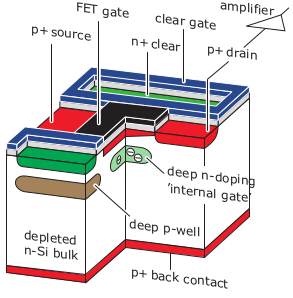
\includegraphics[width=7cm]{Bilder/DEPFET}
	\end{center}
\caption[DePFET]{Illustration of the DePFET technology.\cite{B2TR}}
\label{fig:DePFET}
\end{figure}

A cross section of the device is shown in figure \ref{fig:DePFET}. The structure of a DePFET cell consists of fully depleted silicon. In this silicon substrate, depleted by a high negative voltage, a $p-$channel MOSFET (metal oxide semiconductor field effect transistor) of a JFET (junction field effect transistor) is integrated. The field effect transistors act as a first pre-intensification. When radiation or a particle hists the detector, electron-hole pairs are created. These pairs get separated by the potential field of the sidewards depletion. The positive charged holes drift to the negatively charged back contact. The negative charged electrons are collected in the potential minimum. The so-called internal gate. Above the internal gate a field emission transistor is located. The signal charge is amplified right above the position where it was generated. This avoids the leakage of lateral charge transfers. One of the most important main features of the DePFET is that the internal gate has a very small capacitance. This makes it possible to measure events affected by low noise even at room temperature.\cite{B2TR}

\subsection{Silicon Vertex Detector}
\label{sec:Silicon}

The SVD consists of four layers of double-sided strip detectors. The layers are located at radii of 38, 80, 115 and 140$\,\textrm{mm}$. There are two different shapes of these sensors. The rectangular sensors are used in the barrel part and the trapezoidal sensors are used in the forward region of the SVD. Each sensor has a thickness of $320\,\mu\textrm{m}$ but the sensors have different dimensions depending on the layer they are located. The barrel sensors in the most inner layer of the SVD have a dimension of $38.4 \times 122.8\,\textrm{mm}^2$. The size for the barrel sensors of the other layers is $57.6 \times 122.8\,\textrm{mm}^2$. The trapezoidal sensors have a dimension of $38.4\,\textrm{mm}$ on the small side of the trapeze to $57.6\,\textrm{mm}$ on the long side of the trapeze times a length of $122.8\,\textrm{mm}$.\cite{B2TR} An illustration of the SVD can be seen in figure \ref{fig:SiliconVertex}. 

\begin{figure}[h!]
	\centering
	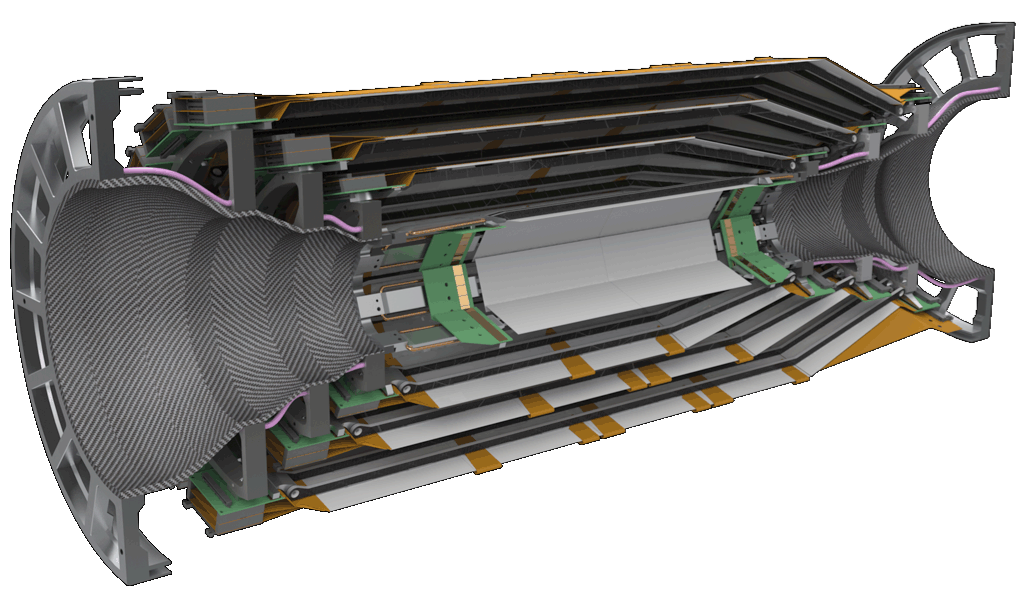
\includegraphics[width=\textwidth]{Bilder/SVD.png}
	\caption[Silicon Vertex Detector]{Cross section of the silicon vertex detector\cite{SVDItalian}}
	\label{fig:SiliconVertex}
\end{figure}

In the barrel region the $p$-side of the double-sided-strip sensors is arranged parallel to the beam axis and facing the interaction region. The $n$-side is facing outside the detector and the $n$-strips are perpendicular arranged to the beam axis. 

When a particles travels through the sensors it creates electron-holes pairs along its path by ionization. The electrons then propagate to the $n$-strips and are accumulated there. The holes propagate to the $p$-strips and are collected there. The sensors then produce a signal from which the coordinate of the particle position can be read out. The $p$-side provides the $z$-direction and the $n$-side provides the $r-\theta$ direction.\cite{B2TR} \cite{bergauer2010silicon}



\section{Central Drift Chamber}
\label{sec:CDC}

The CDC surrounds the SVD. It consists of 14336 wires arranged in 56 layers and has an inner radius of $16\,\textrm{cm}$ and an outer radius of $113\,\textrm{cm}$. The volume is filled with a $50\,\%\,\textrm{helium}$ and an $50\,\%\,\textrm{ethane}$ gas mixture. The purpose of the CDC is to reconstruct the momenta and tracks of charged particles, to identify these particles by measuring their specific energy loss within the gas volume. The CDC alone is able to identify low-momentum tracks, which are unable to reach the particle identification device. The CDC also acts as a reliable trigger for charged particles.\cite{B2TR} A small cross section of the CDC is shown in figure \ref{fig:CDC}.

\begin{figure}[h!] 
	\centering
	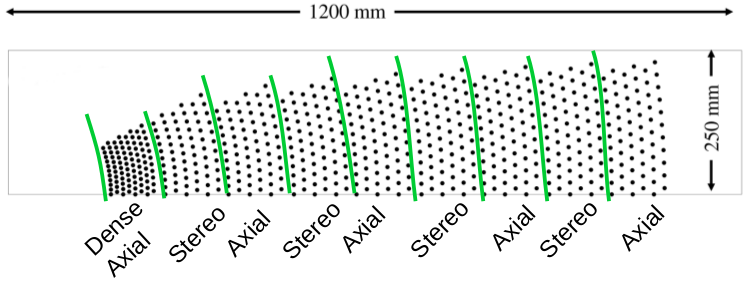
\includegraphics[width=\textwidth]{Bilder/CDC}
	\caption[Central Drift Chamber]{Cross section and only a small part of the CDC. Each dot represent a wire. Also the area for the different superlayers are separated by the green line. All of these wires are immersed in a helium-ethane mixture.\cite{CDCHauth}}
	\label{fig:CDC}
\end{figure}

When a charged particle passes through the CDC it losses energy due to ionization of the gas. This produces electron-ion pairs, which are then separated by the electric field provided by 42240 aluminum field wires, with a diameter of $125\,\mu\textrm{m}$. The signal is then read out by the sense wires. These have a radius of $30\,\mu\textrm{m}$ and are made out of gold-plated tungsten.\cite{B2TR} 

As indicated in figure \ref{fig:CDC} there are different superlayers in the CDC. The Dense Axial and Axial sense wires allow the reconstruction of the track in the $r-\phi$ plane. The stereo sense wires gives information about the $z$ direction. These stereo wires are tilted in respect to the $z$ direction. Six layers of sense wires are combined to a superlayer. The CDC consists of five axial superlayers (A), and four stereo superlayer. The four stereo superlayer subdivide into two stereo superlayer (U) with a positive stereo angle and two stereo superlayers (V) with a negative stereo angle. Starting with the innermost superlayer, every second superlayer is an axial superlayer. The stereo superlayers are between them, alternating between U and V. In total there are nine superlayers. The innermost superlayer is called \textit{small-cell chamber} has a total of eight superlayers. (compared to the other superlayers with just six layers) This was done to lower the influence of the background, which is higher in the innermost superlayer due to the vicinity to the interaction region.
The CDC has a spatial resolution of about $100\,\mu\textrm{m}$.\cite{B2TR}

\section{TOP And ARICH}
\label{sec:ARTO}

There are two additional detectors for particle identification, the TOP and the ARICH. The TOP counter is located in the barrel part and it uses a combination of time-of-flight and Cerenkov angle measurements.
When a charged particle with the velocity $\beta$ is faster than the speed of light $c_n$ in a medium  with a reflective index $n$ then this particle emits Cerenkov radiation under the angle $\theta_{C} $.\cite{cerenkovAngle}


\begin{equation}
c_n = \frac{c_0}{n} \leq \beta	
\end{equation}

The Cerenkov angle is given by:\cite{cerenkovAngle}

\begin{equation}
\textrm{cos}(\theta_C)=\frac{1}{n\beta}
\end{equation}

\begin{figure}[h!]
	\centering
	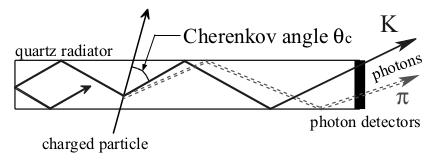
\includegraphics[width=12cm]{Bilder/TOP}
	\caption[TOP Principle]{Operating mode of a TOP detector.\cite{B2TR}}
	\label{fig:TOP}
\end{figure}

Figure \ref{fig:TOP} shows an illustration of the functionality of a TOP bar. The charged particle emits Cerenkov light when it passes the quartz crystal. These photons then travel inside the crystal due to reflection until they are detected by a photon detector. Measuring the time difference between the emitted photons it is possible to calculate the position of the track of the charged particle. The outgoing photons are then focused by mirrors and are then detected by PMTs. Cerenkov photons with different $\theta_C$ will be detected by different PMTs. Therefore, the TOP reconstruct the Cerenkov ring image using the information of time, $x$ and $y$.\cite{B2TR} 

The TOP counter consists of 32 quartz bars. They have a length of $1250\,\textrm{mm}$, a width of $45\,\textrm{mm}$ and a depth of $20\,\textrm{mm}$. There are two quartz bars per module. The TOP counter has a $K/\pi$ separation of over $99\,\%$.\cite{B2TR}

The ARICH detector is located in the forward end-cap region. It is designed to distinguish between kaons and pions over most of their momentum spectrum. It is also able to identify particles with a momentum below $1\,\textrm{GeV}$.

\begin{figure}[h!]
	\centering
\begin{minipage}[b]{0.45\linewidth}
	\centering
	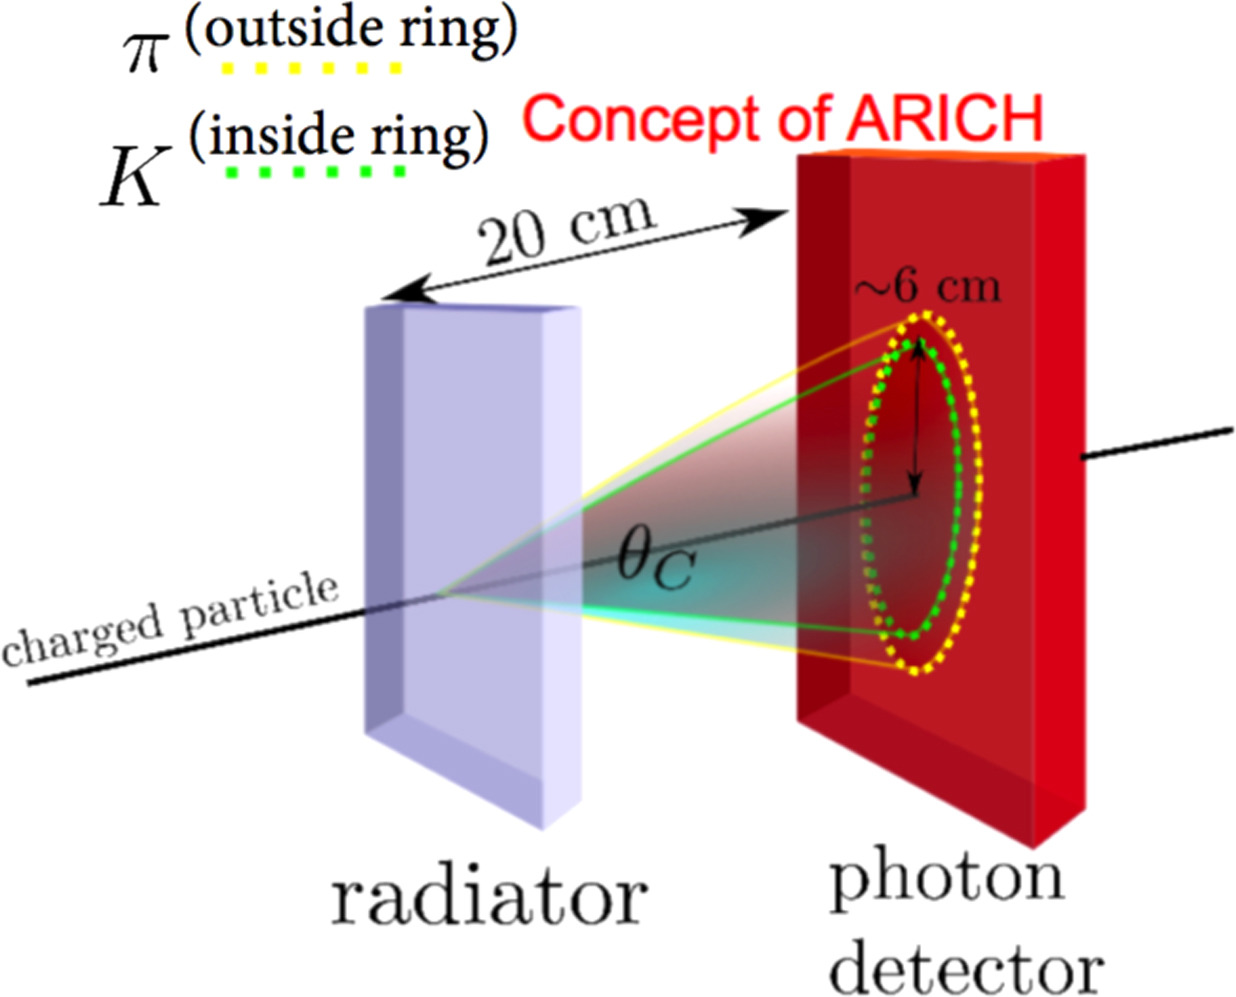
\includegraphics[width=\textwidth]{Bilder/ARICH}
\end{minipage}
\hspace{0.5cm}
\begin{minipage}[b]{0.45\linewidth}
	\centering
	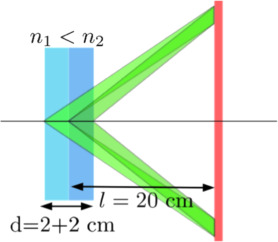
\includegraphics[width=\textwidth]{Bilder/ARICH2}
\end{minipage}

	\caption[ARICH]{Left: Illustration of the working principle of the ARICH detector. The yellow Cerenkov ring on the photon detector is produced by a $\pi$, the green ring by a $K$. Right: The radiator is shown in more detail. The radiator consists of two aerogel layers with different reflective index. \cite{TORASSA} }
\label{fig:ARICH}
\end{figure}

In figure \ref{fig:ARICH} the working principle of the ARICH detector is shown. A charged particle passes through two layers of an aerogel radiator with different reflective indexes and emits Cerenkov photons under a Cerenkov angle $\theta_C$. Behind the radiator is an extension volume for the Cerenkov rings to form. At a distance of $20\,\textrm{cm}$ behind the radiator is the photon detector.\cite{B2TR} Once the Cerenkov ring is reconstructed, the radius of the ring can be determined and, knowing the distance and the radius, the Cerenkov angle can be calculated.

\section{Electromagnetic Calorimeter}
\label{sec:ECL}

One of the main tasks of the ECL is the detection of photons with a high efficiency. It also determents the energy and the angular coordinates of these photons with high precision. It is also used for electron identification and the generation of a proper signal for the trigger. The ECL consists of a $3\,\textrm{m}$ long barrel section with an inner radius of $1.25\,\textrm{m}$. The circular end-caps are located at a distance of $z=1.96\,\textrm{m}$ in the forward direction and $z=-1.02\,\textrm{m}$ in the backward direction from the interaction point. The ECL covers a polar angle region of $12.4^{\circ} < \theta < 155.1^{\circ}$. Due to construction, there are two $ \sim 1^{\circ}$ wide gaps between the barrel and the end-caps. The barrel section of the calorimeter consists of 6624 CsI(Tl)\footnote{Thallium activated Cesium Iodide} crystals with 29 distinct shapes. Each of these crystals is a truncated pyramid with an average size of about $6\times6 \, \textrm{cm}^2$ in cross section and $30\,\textrm{cm}$ in length. The length of these crystals corresponds to around 16.1 radiation lengths $X_0$. The end-caps consist of 2122 CsI crystals of 69 shapes. At the end of each crystal, photo-multiplier are mounted to detect the excitation of the scintillators. The detected number of photons corresponds directly to the energy released by absorbed particles.
The energy resolution of the calorimeter can be approximated as:\cite{B2TR} \cite{Belle_ECL_2015}

\begin{equation}
\frac{\sigma_E}{E} = \sqrt{\bigg(\frac{0.066\%}{E}\bigg)^2 + \bigg(\frac{0.81\%}{\sqrt[4]{E}}\bigg)^2 + (1.34\%)^2}
\end{equation}
The energy E is in GeV.
\newline

Photons and electromagnetic particles are creating electromagnetic cascades when they pass through material.\cite{leo2012techniques} When a high energetic photon passes through a material it creates an electron-positron pair by pair production. For this, the photon must have at least an energy of $2\cdot m_{e^{-}} = 1.022\,\textrm{MeV}$. This energy is evenly distributed between the two particles. Because these two particles are charged and their velocity changes in an the electric field of a nuclei, they generate photons through Bremsstrahlung. These processes are repeated and an electromagnetic shower is created. The energies of the particles continue to decrease until the critical energy $E_c$ is reached. At the critical energy, the energy loss due to Bremsstrahlung is as high as the energy loss due to ionization.

If the average energy of an electron becomes ${E_0}/{e}$ then the distance the electron traveled is called radiation length $X_0$.

Assuming that the electromagnetic particles and photons interact after one radiation length and that they loose half of their energy each time they do, the total number of particles and their energy after $t$ cascades can then be calculated by:\cite{leo2012techniques}

\begin{equation}
	N \simeq 2^t
\end{equation}

\begin{equation}
	E(t) \simeq \frac{E_0}{2^t}
\end{equation}

This shower both spreads longitudinally and transversely. The transverse propagation can be described by the Moli\`ere radius. It can be calculated by:

\begin{equation}
	R_M=21\,\textrm{MeV}\cdot \frac{X_0}{E_c}
\end{equation}

$ 95\,\%$ of all particles of a shower are within two Moli\`ere radii.\cite{leo2012techniques}

\section{$K_L^0$ And Muon Detector }
\label{sec:KM}

The KLM consists of an alternating sandwich structure of a $4.7\,\textrm{cm}$ thick iron plates and resistive plate chambers (RPC) in between.

RPCs consist of two glass sheets, separated by a thin gas volume. These sheets act as high voltage electrodes. When a particle passes through the volume, they create ion-electron pairs which are then accelerated by the strong electric field. Therefore, they initiate more ionizations, which leads to a streamer between the electrodes. This causes a voltage drop in the nearby electrodes, which is detected by pick-up strips, located on both sides of the chamber. These strips are a few centimeters wide and are placed orthogonal on each side. Therefore, the particle track can be localized in $z/\phi$ for the barrel region and $\phi/\theta$ for the end-caps.

To distinguish between muons and hadrons, the KLM takes advantage of the high penetration power of muons. Hadrons deplete their energy through hadronic showers in the ECL and KLM. Electrons have a shorter radiation length and are therefore absorbed by the ECL, most of the time. $K_L^0$ create clusters in the ECL and the KLM. These clusters are than grouped and geometrically matched to charged tracks which are detected by the inner detectors. If no corresponding charged track can be found by geometrical matching, the detected particle is then treated as a $K_L^0$ candidate.\cite{B2TR}\cite{KLMS}



\chapter{Trigger And Data Acquisition System}
\label{sec:TDAS}


\lettrine{I}{n} this chapter a short introduction to the trigger system and the data acquisition system at Belle II is provided.


\section{Trigger}

The online event selection system (trigger) for Belle II makes it possible to acquire data from the detector based on information from a set of sub-detectors. The individual triggers are structured in an hierarchy. Each sub-trigger system provides the trigger information from the corresponding sub-detector to the global decision logic (GDL). This global trigger finally decides whether the event should be written out or not. \cite{B2TR} A schematic overview of this trigger hierarchy can be found in figure \ref{fig:Trigger}.


\begin{figure}[h!]
	\centering
	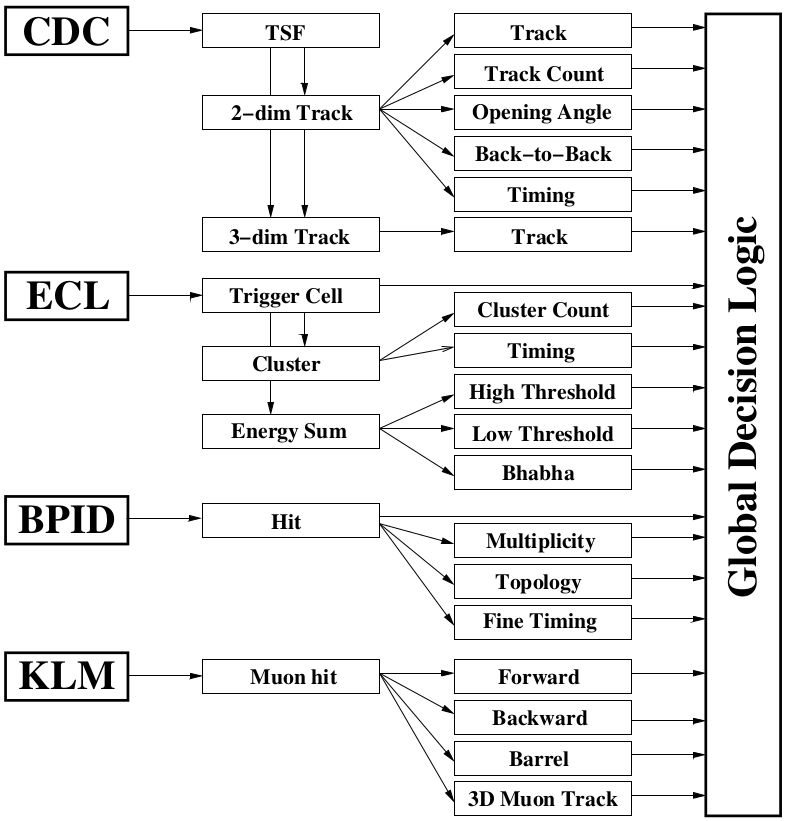
\includegraphics[width=\textwidth]{Bilder/Trigger}
	\caption[Schematic Overview Of The Trigger System]{Schematic overview of the Belle II trigger system. The four sub-trigger systems send their outputs to the Global Decision Logic. The GDL then performs the final on-line trigger decision. \cite{LumiTrigger}}
	\label{fig:Trigger}
\end{figure}




The trigger system has to fulfill the following requirements:\cite{B2TR}

\begin{enumerate}
	\setcounter{enumi}{-1}
	\item high efficiency for hadronic events from $\Upsilon(4\textrm{S}) \rightarrow B\bar{B}$ and from continuum
	\item a maximum average trigger rate of $30\,\textrm{kHz}$
	\item a fixed latency of about $5\,\mu \textrm{s}$
	\item a timing precision of less than $10\,\textrm{ns}$
	\item a minimum two-event separation of $200\,\textrm{ns}$
	\item a trigger configuration that is flexible and robust
\end{enumerate}


At SuperKEKB bunch crossing occurs almost continuously, since the radio-frequency (RF) is about $508\,\textrm{Hz}$ and every second or third period produces an event.\cite{B2TR} The total cross section and trigger rates at a luminosity of  $	\mathcal{L} = 8\cdot 10^{35} \, \textrm{cm}^{-2} \textrm{s}^{-1}$ for various physics processes is shown in table \ref{tab:Lumi}.



\begin{table}[h!]
	\centering
\begin{minipage}{\textwidth}
\renewcommand{\thefootnote}{\emph{\alph{footnote}}}
\begin{center}

		\begin{tabular}{ccc}


 Physics process&Cross section (nb) &Rate (Hz) \\
 \hline
$\Upsilon(\textrm{4S} \rightarrow B\bar{B}$) & 1.2&960 \\
 $\textrm{e}^+ \textrm{e}^- \rightarrow \textrm{continuum}$&2.8 &2200 \\
 $\mu^+ \mu^-$&0.8 &640 \\
 $\tau^+ \tau^-$&0.8 &640 \\
 $\textrm{Bhabha} \,\,(\theta_{\textrm{lab}} \geq 17^{\circ})$ &44 &350 \footnote{\label{note1}The rate is pre-scaled by a factor of 1/100}\\
 
 $\gamma \gamma \,\,(\theta_{\textrm{lab}} \geq 17^{\circ})$& 2.4&19 \footref{note1} \\
 $2\gamma \,\,\textrm{processes } (\theta_{\textrm{lab}} \geq 17^{\circ},\,\, p_t \geq 0.1\,\textrm{GeV/c} )$&$\sim 80$ &$\sim 15000$ \\
 \hline
 Total& $\sim 130$& $\sim 20000$\\
		\end{tabular}

	\caption[Luminosity at Belle II]{Total cross section and trigger rates for $\mathcal{L} = 8\cdot 10^{35} \, \textrm{cm}^{-2} \textrm{s}^{-1}$ from various physics processes at the $\Upsilon(4\textrm{S})$.\cite{LumiTrigger}}
	\label{tab:Lumi}

\renewcommand{\thefootnote}{\arabic{footnote}}
\end{center}
\end{minipage}
\end{table}

The luminosity is measured by using Bhabha and $\gamma \gamma$ events. These events are also used to calibrate the detector response. Due to the high luminosity, these events are very dominant. That is the reason why there is a prescaling factor of 100  on these events. This means that on  predetermined fraction of these events are accepted after satisfying the trigger requirements.
After a beam collision, the GDL decides within about $5\,\mu \textrm{s}$ if the event should be accepted and if it should be written out. Since the GDL is the first module to make a decision, and since it is dead time free, it is also called Level-1 trigger.\cite{B2TR}

\section{Data Acquisition System}
\label{sec:DAQ}

The data acquisition system (DAQ) reads out the detector signals once the Level-1 trigger decision is given by the trigger system. Starting from the front-end electronics, DAQ transfers the data trough multiple steps of data processing to the storage system. With the exception of the PXD, all sub-detectors are read out by the unified data link system called the Belle2Link. The working principle of the DAQ can be seen in figure \ref{fig:DAQ}.

\begin{figure}[h!]
	\centering
	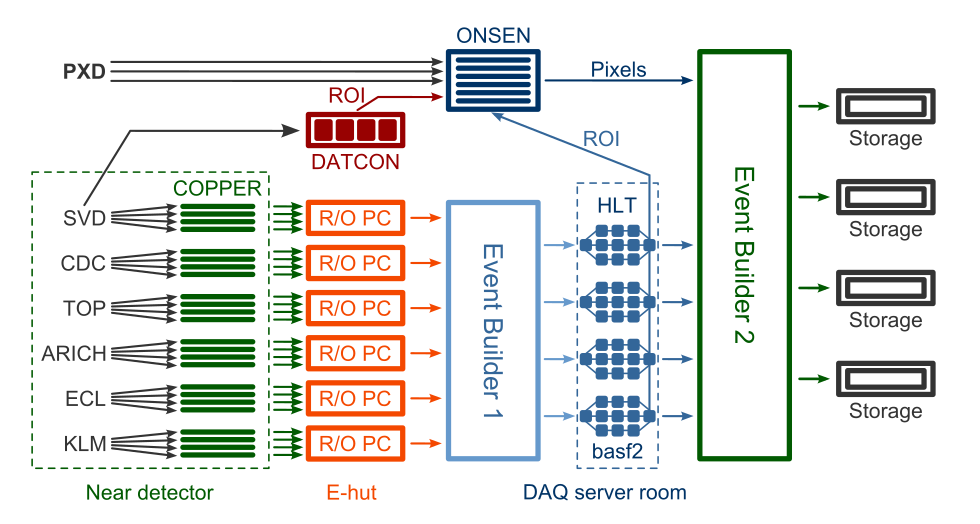
\includegraphics[width=\textwidth]{Bilder/DAQ}
	\caption[Working Principle of the DAQ]{Working principle of the Belle II DAQ. The data is transfered by about 300 COPPER boards to about 30 R/O PCs. The data is then put together by the first event builder and the events are reconstructed by the HLT afterwards. The HLT contains $O(10)$ units with about 400 cores each. Then, the reconstructed data is merged with the data coming from the PXD. Finally, the data is saved on about 10 storage units. \cite{Filippo:1097}}
	\label{fig:DAQ}
\end{figure}

The first part of the Belle2Link is the common readout platform (COPPER). This platform transforms the different data formats coming from the sub-detectors into a common data format. The COPPER boards then send their output signal to the event builder, which merges the data coming from the same collision to an event. With the information from the fully reconstructed events, the high level trigger (HLT) is able to finally decide whether the event should be stored or not. If the event should be recorded, it is then merged with the information coming from the PXD data in the second event builder.

Once the PXD receives the trigger signal, the readout starts. These data are stored on on-line selector nodes for up to $5\,\textrm{s}$. Meanwhile, the HLT performs the event reconstruction. Based on information coming from the SVD and CDC, the charged tracks, reconstructed in the HTL, are transfered back to the PXD and regions of interest (ROI) are formed. Only pixels of the PXD within the ROI are kept and considered in the second event builder. Complementarity to the HLT, the data concentrator also searches for RIOs. The HLT is optimized for high momentum and the data concentrator is optimized for low momentum particles. Both systems require hits in all SVD layers. 





\chapter{BASF2}
\label{sec:Tools}

\lettrine{T}{he} software framework used at Belle II is called BASF2 (Belle AnalysiS Framework). It is designed to prosecute off-line and analysis tasks. The majority of the code is written in C++, but python scripts are used for framework execution. The user specifies a sequence of modules in the python steering file which than process events. It also provides access to external libraries like ROOT which allows processing, statistical analysis, visualization and storage of common data and Geant4 for simulating the full detector.\cite{Moll_2011}


For the off-line reconstruction to work it has to take into account that the Belle II detector consists of a set of subdetectors. Each subdetector has a different geometry, dimension and is made out of different materials buried in a magnetic field. It also exploits the informations on the interactions of the particles with the matter. These informations are then used to reconstruct the particle trajectories (tracks) and the signal they generate in the detectors. This is done using algorithm that model particle propagation.








\chapter{Preparation  For Calculating The Tracking Efficiency Of Phase2}
\label{chap:Phase2Eff}

\lettrine{T}{his} chapter will provide an overview on how the cuts where chosen and which selection was applied in order to calculate a reasonable tracking efficiency on phase2 data. We will start with a definition of the tracking efficiency we want to calculate. Then the reconstruction and selection of the Bhabha events using only ECL informations will be described. The same selection and cuts used on phase2 will also be used on phase3 later on.

\section{Phase2}
\label{sec:Phase2}

Phase2 data were taken in the time between March 2018 and July 2018. During this time, only a small azimuthal fraction of the vertex detector was installed. A sketch of the installed VXD can be found in the appendix figure \ref{fig:phase2vxd}. The main focus of this phase was to study the background of the newly installed Belle II detectors, in order to be certain that the operation of the vertex detector is compatible with the much higher luminosity expected for physics data taking. Also, hardware controls were tested in this phase.


\section{Definition Of Tracking Efficiency}
\label{sec:Eff}

First of all, a definition of efficiency has to be declared, since there are different ways to define a tracking efficiency. The physics case we are considering is Bhabha events $ \textrm{e}^+ \textrm{e}^- \rightarrow \textrm{e}^+ \textrm{e}^- $. As described in chapter \ref{sec:SetupKEK}, charged particles leave a track in the detector. So, when we look at an outgoing particle with a track, then we know that the other particle should also have a track. If the other particle has no track associated, then this is an inefficiency. If both particles have a track associated, then this is the efficient case.

So for this work, we will use the following definition for the tracking efficiency:

\begin{equation}
	\epsilon = \frac{\textrm{Number of Bhabha events with exactly 2 reconstructed tracks}}{\textrm{Number of Bhabha events with 1 or more reconstructed tracks}}
	\label{eq:efficiency}
\end{equation}


To calculate an efficiency according to equation \ref{eq:efficiency} one needs two histograms. One histogram filled particle information in the case that both particles are charged, and a histogram filled with particle information in the case that at least one particle in the event is reconstructed as a charged particle. The first will be referred to as \textit{enumerator} histograms and the later will be referred to as \textit{denominator} histograms.


The particle we investigate will be called \textit{probe}. The other particle will be called \textit{tag}. We  know that \textit{tag} is always reconstructed as a charged particle. Therefore, we will calculate the efficiency for two different cases:

\begin{itemize}
	
	\item Electron: \textit{tag} is reconstructed as a positron
	\item Positron: \textit{tag} is reconstructed as an electron
\end{itemize}





\section{Reconstructing Bhabha Events With Basf2}
\label{sec:RecBasf2}


To analyze a Monte Carlo (MC)  or data file, a python script using Basf2 has to be written. The following code is a simplified version of the steering file I wrote. 
The whole steering file is located on KEKCC at:


/home/belle2/msobotzi/bhabha/bhabha\_vpho.py
\newline


The goal of this steering file is to reconstruct the virtual photon in a Bhabha event. This virtual photon decays into two daughters which hit then the ECL. Since we want to calculate the tracking efficiency, we need to be able to reconstruct the virtual photon from two daughters both associated with a track, and two daughters one associated with a track (reconstructed as a charged particle by the framework) and one with no track associated (reconstructed as a photon by the framework).

The same steering file is used for data and MC.
\newline 





{\small
\begin{lstlisting}
fillParticleList('gamma:all', 'clusterE > 0.01', path=mypath)
fillParticleList('e+:all', 'clusterE > 0.01', path=mypath)

reconstructDecay('vpho:gamma -> gamma:all', '', path=mypath)
reconstructDecay('vpho:elec -> e+:all', '', path=mypath)

copyLists(outputListName = 'vpho:ECLObjectUnranked' ,inputListNames=['vpho:elec', 'vpho:gamma'], path=mypath)

rankByHighest('vpho:ECLObjectUnranked', 'daughter(0,clusterE)', path=mypath)
cutAndCopyList('vpho:ECLObject', 'vpho:ECLObjectUnranked', '', path=mypath)
	
reconstructDecay('vpho:bhabha -> vpho:ECLObject vpho:ECLObject', '', path=mypath)

variablesToNtuple('vpho:bhabha', variables, treename = 'vpho_bhabha', filename = output.root, path=mypath)
	
\end{lstlisting}
}
\bigskip







In the first line of code all particles which hit the ECL and have no track associated are filled into a gamma list called \texttt{gamma:all}. The clusters created by those particles must have an energy (clusterE) of at least $0.01\,\textrm{GeV}$. In the second line a list called \texttt{e+:all} is created. All particles with an associated track are filled in this list independently of their charge. Therefore, this list contains for example electrons, positrons and even muons. Therefore, a cut is applied to the cluster energy and not on the energy of the particles.


Due to the fact, that we want to calculate the efficiency of the tracking, we need to somehow combine the \texttt{e+:all} and the \texttt{gamma:all} lists. As mentioned earlier, we need to be able to reconstruct the virtual photon from particles reconstructed as electrons/positrons and photons.
Unfortunately, the Basf2 framework prevents a combination of two different particle lists, like \texttt{e+:all} and \texttt{gamma:all}. Therefore, we need to use a trick. This is shown in lines four and five. In line four, we tell the framework that the reconstructed gamma is the only daughter of a virtual photon called \texttt{vpho:gamma}. The same is done for the electron list. Here, the virtual photon is called \texttt{vpho:elec}. 

Now, these two lists can be combined to one list called \texttt{vpho:ECLObjectUnranked}. This is done in line seven.

In line nine and ten the daughters in the \texttt{vpho:ECLObjectUnranked} list are sorted by their cluster energy and filled in a list called \texttt{vpho:ECLObject}.

In line twelve, the virtual photon of the Bhabha event is reconstructed from the ECL objects in the \texttt{vpho:ECLObject} list. The number of reconstructed virtual photon candidates per event $n_{\textrm{cand}}$ is determined by the following equation\cite{triangular}:

\begin{equation}
n_{\textrm{cand}} = \frac{n_{\textrm{p}}(n_{\textrm{p}} +1)}{2}
\label{eq:Triangular}
\end{equation}

$n_{\textrm{p}}$ is the number of reconstructed particles per event. Equation \ref{eq:Triangular} is also known as the equation to calculate \textit{triangular numbers}. For example, if four ECL particles are reconstructed in a single event then ten virtual photon candidates are reconstructed according to equation \ref{eq:Triangular}. Since we only expect one virtual Bhabha photon per event, we have to select the best candidate in each event. This will be done in section \ref{sec:SelectingBhabhaMC}.

Since the entries in the \texttt{vpho:ECLObject} list are sorted by energy, the first daughter of the reconstructed virtual Bhabha photon always has a higher energy than the second daughter. The first daughter will be refered to as \texttt{HclE} and the second daughter as \texttt{LclE}. You can see that the \texttt{HclE} daughter has always a higher energy than the \texttt{LclE} daughter in figure \ref{fig:clEDiff}. Here the clusterE(\texttt{LclE}) is subtracted from the clusterE(\texttt{HclE}) and only positive values remain. Therefore, \texttt{HclE} is the daughter with the higher energy.

Finally, in the last line of code, all variables of the candidates like mass, momentum, cluster energy of each daughter, does the daughter have a track and so on are written in a tree \texttt{vpho\_bhabha} in a file. The \texttt{outputname} of the output file depends on whether the steering file is running on data or MC. 


\section{Best Candidate Selection On Phase2 Monte Carlo}
\label{sec:SelectingBhabhaMC}

We use Monte Carlo simulation due to the fact that on MC we know everything about the generated and reconstructed particles. So on MC we can select Bhabha events which hit the ECL and with this knowledge we can introduce cuts in such a way that we only reconstruct these Bhabha events. To calculate an efficiency it is extremely  important to select only Bhabha events. At first, we are also running on only one $\textrm{e}^+ \textrm{e}^- \rightarrow \textrm{e}^+ \textrm{e}^-$ MC file which is located on KEKCC at:
\newline

/belle/MC/release-01-00-02/DB00000294/MC10/prod00004668/s00/e1002/4S/
r00000/3600520000/mdst/sub00/mdst\_000050\_prod00004668\_task10010000050.root
\newline

The generated file is located at:

 /home/belle2/msobotzi/bhabha/bhabha\_vpho\_mc.root
\newline


\subsection{CDC-Cut}

Due to the fact that charged particles are reconstructed using informations coming from the CDC detector, we are only interested in events which would pass the CDC. So, we apply a $\theta$-cut on the generated daughters (generated daughters means the true generated Monte Carlo daughters). 
\begin{equation}
	0.296706 < \theta_{HclE,LclE} < 2.617990
\end{equation}

All the events which survive this cut are written into a list (\textit{mcEvtCDC}). We know that the Monte Carlo file contains 140000 generated Bhabha events. After this cut, only 24286 Bhabha events remain.
In section \ref{sec:BhabhaProcess}, we saw that Bhabha events have a very high cross-section in forward and backward  direction. So, we expect that most of the generated daughters are not passing the CDC. 
\newline





Now, we will take a look at the reconstructed Monte Carlo events. All of these reconstructed events have to appear in the mcEvtCDC list because we know that only in these events both daughters are passing the CDC. A total of 24100 events have at least one reconstructed candidate.





\begin{figure}[h!]
	\centering
	\begin{minipage}[b]{0.45\linewidth}
		\centering
		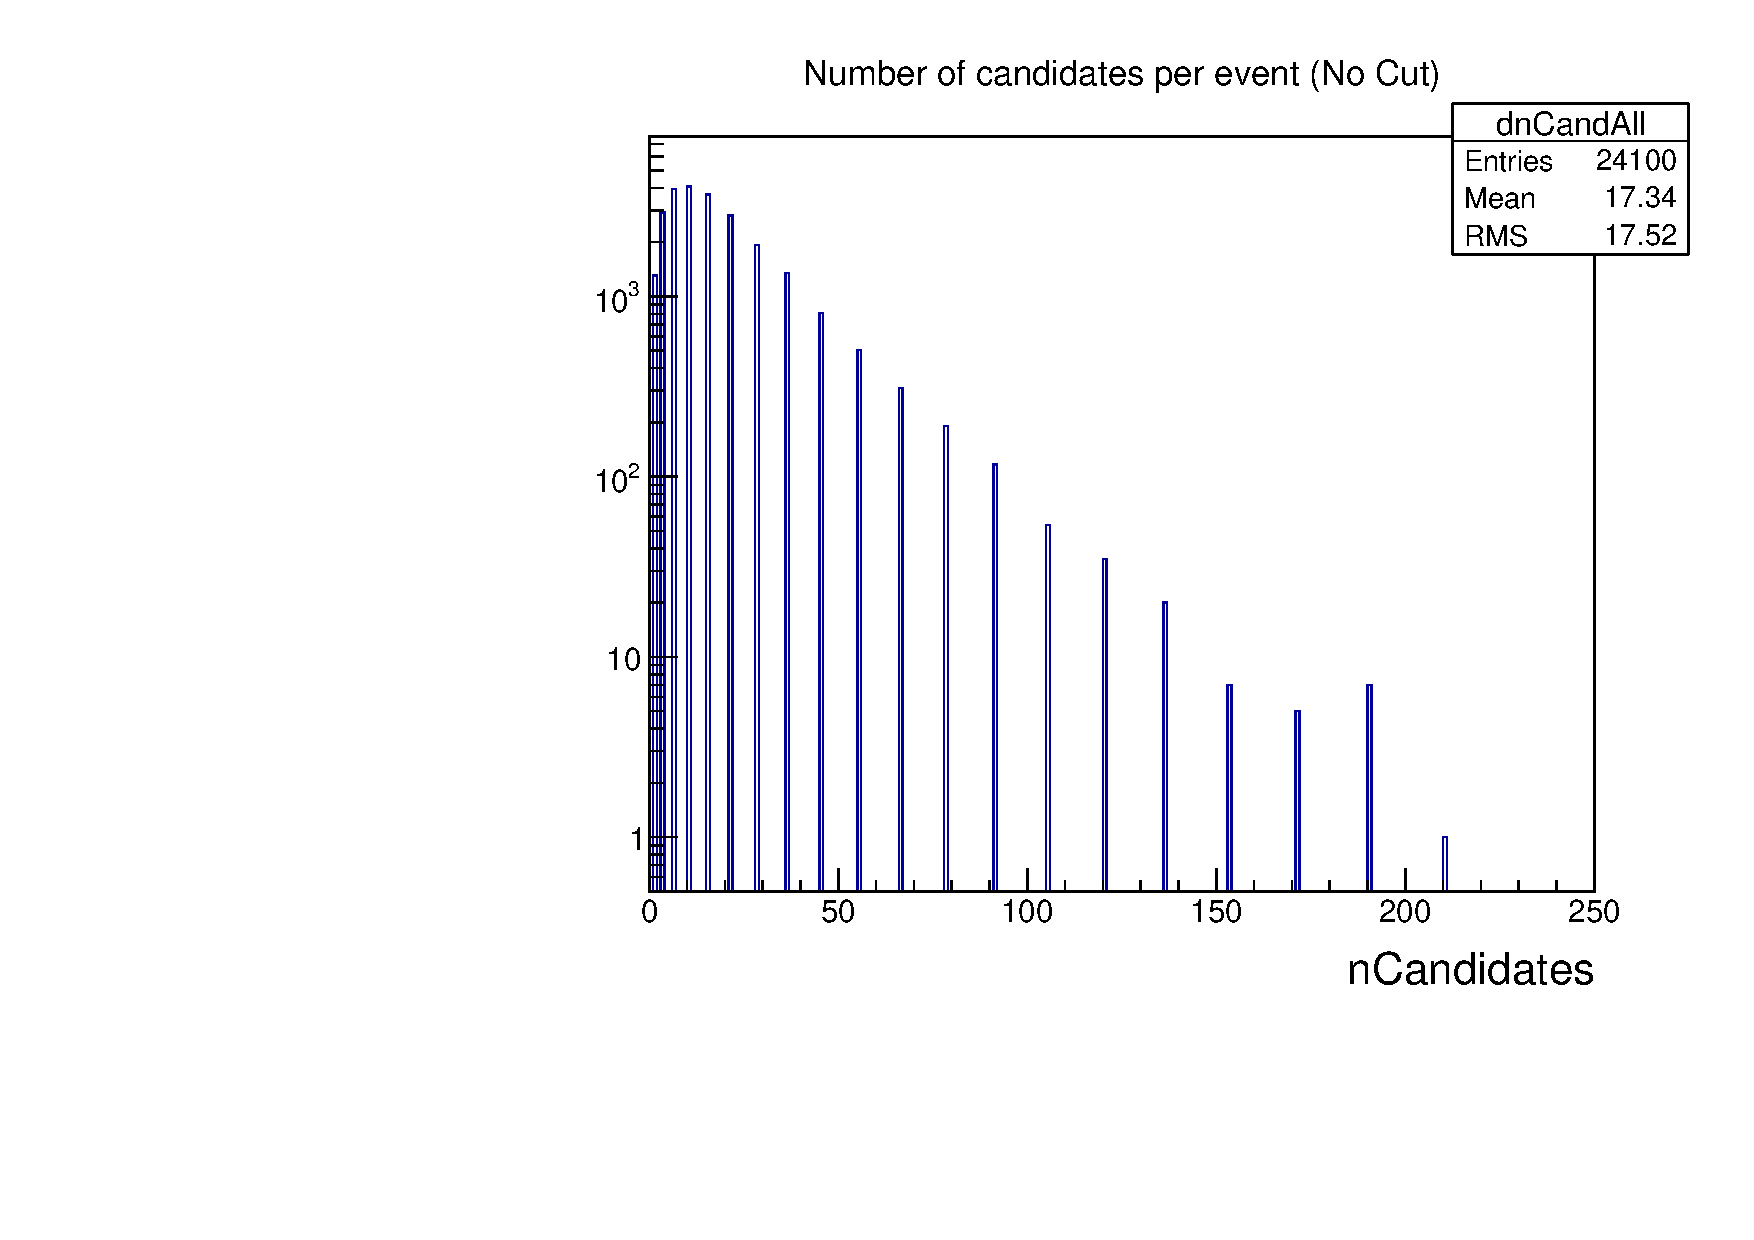
\includegraphics[width=\textwidth]{Cuts/nCandAll.pdf}
	\end{minipage}
	\hspace{0.5cm}
	\begin{minipage}[b]{0.45\linewidth}
		\centering
		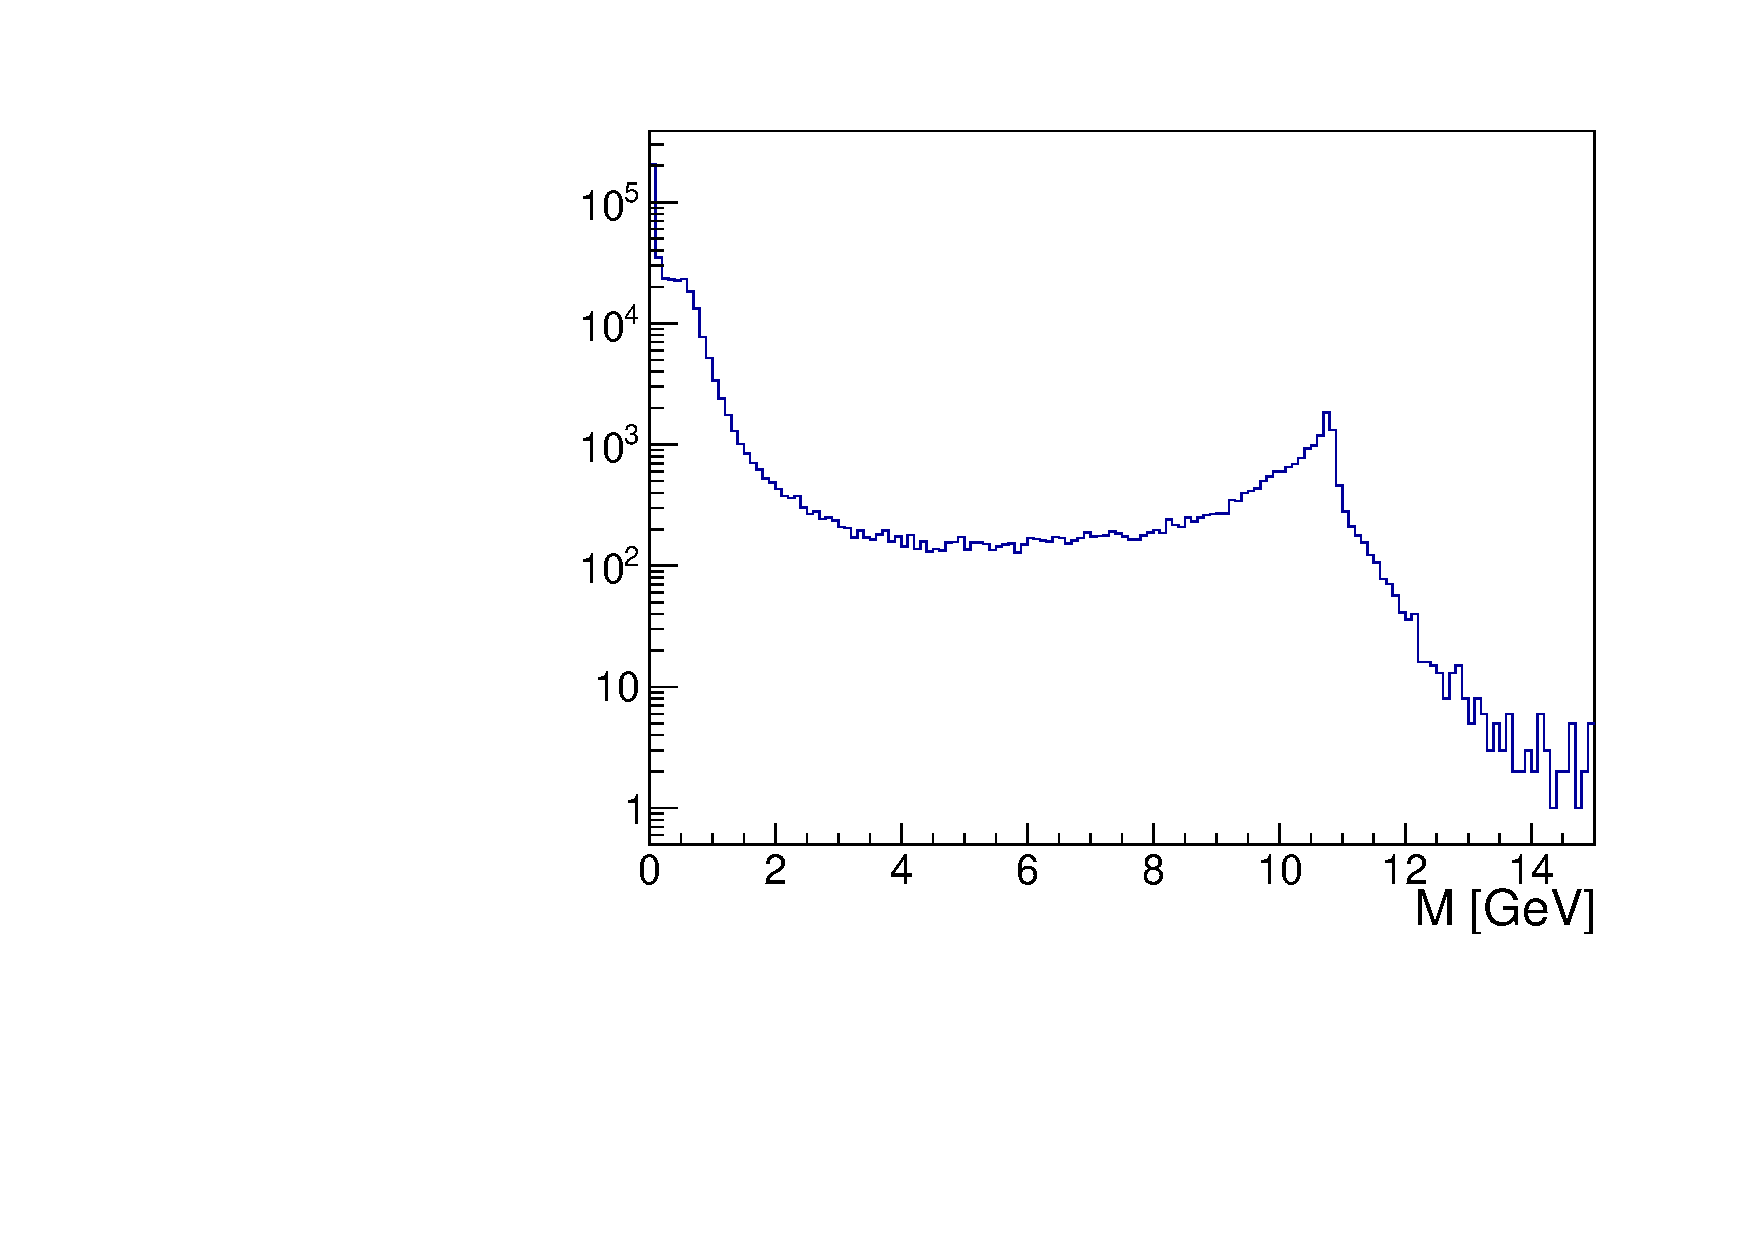
\includegraphics[width=\textwidth]{Cuts/Mall.pdf}
	\end{minipage}
	\caption[Number Of Candidates And Invariant Mass (No Cuts)]{Left: The number of reconstructed candidates per event is shown. We select 24100 events.
		Right: The invariant mass of the reconstructed candidates is shown. We select 417899 candidates.}
	\label{fig:nCandAll}
\end{figure}



In figure \ref{fig:nCandAll} on the left, we see the number of reconstructed candidates per event. Since we do not have a cut on the reconstruction, the number of reconstructed candidates $n_{\textrm{cand}}$ follows equation \ref{eq:Triangular}. On the right, we see the invariant mass of the reconstructed candidates. Note that we are now looking at candidates and as we can see on the left we oftentimes have more than one candidate per event. Therefore, the numbers of entries for the mass is way higher then for the number of candidates per event.
Consequently, we need some cuts to select the best candidate in each event and thereby reduce the number of candidates per event to one.


\subsection{Mass-Cut}

The first cut to reduce the number of reconstructed candidates per event is a mass cut (The cut is called \texttt{M}). As we saw in figure \ref{fig:nCandAll}, a lot of candidates are reconstructed with an low invariant mass and we know from section \ref{sec:BhabhaProcess} that the mass of the reconstructed candidate should be the invariant mass of the collider. For Belle II this is around $10.58\,\textrm{GeV}$. Due to some acceptance for reconstruction error the mass cut is with an lower-cut of $8\,\textrm{GeV}$ rather loose.



\begin{figure}[h!]
	\centering
	\begin{minipage}[b]{0.45\linewidth}
		\centering
		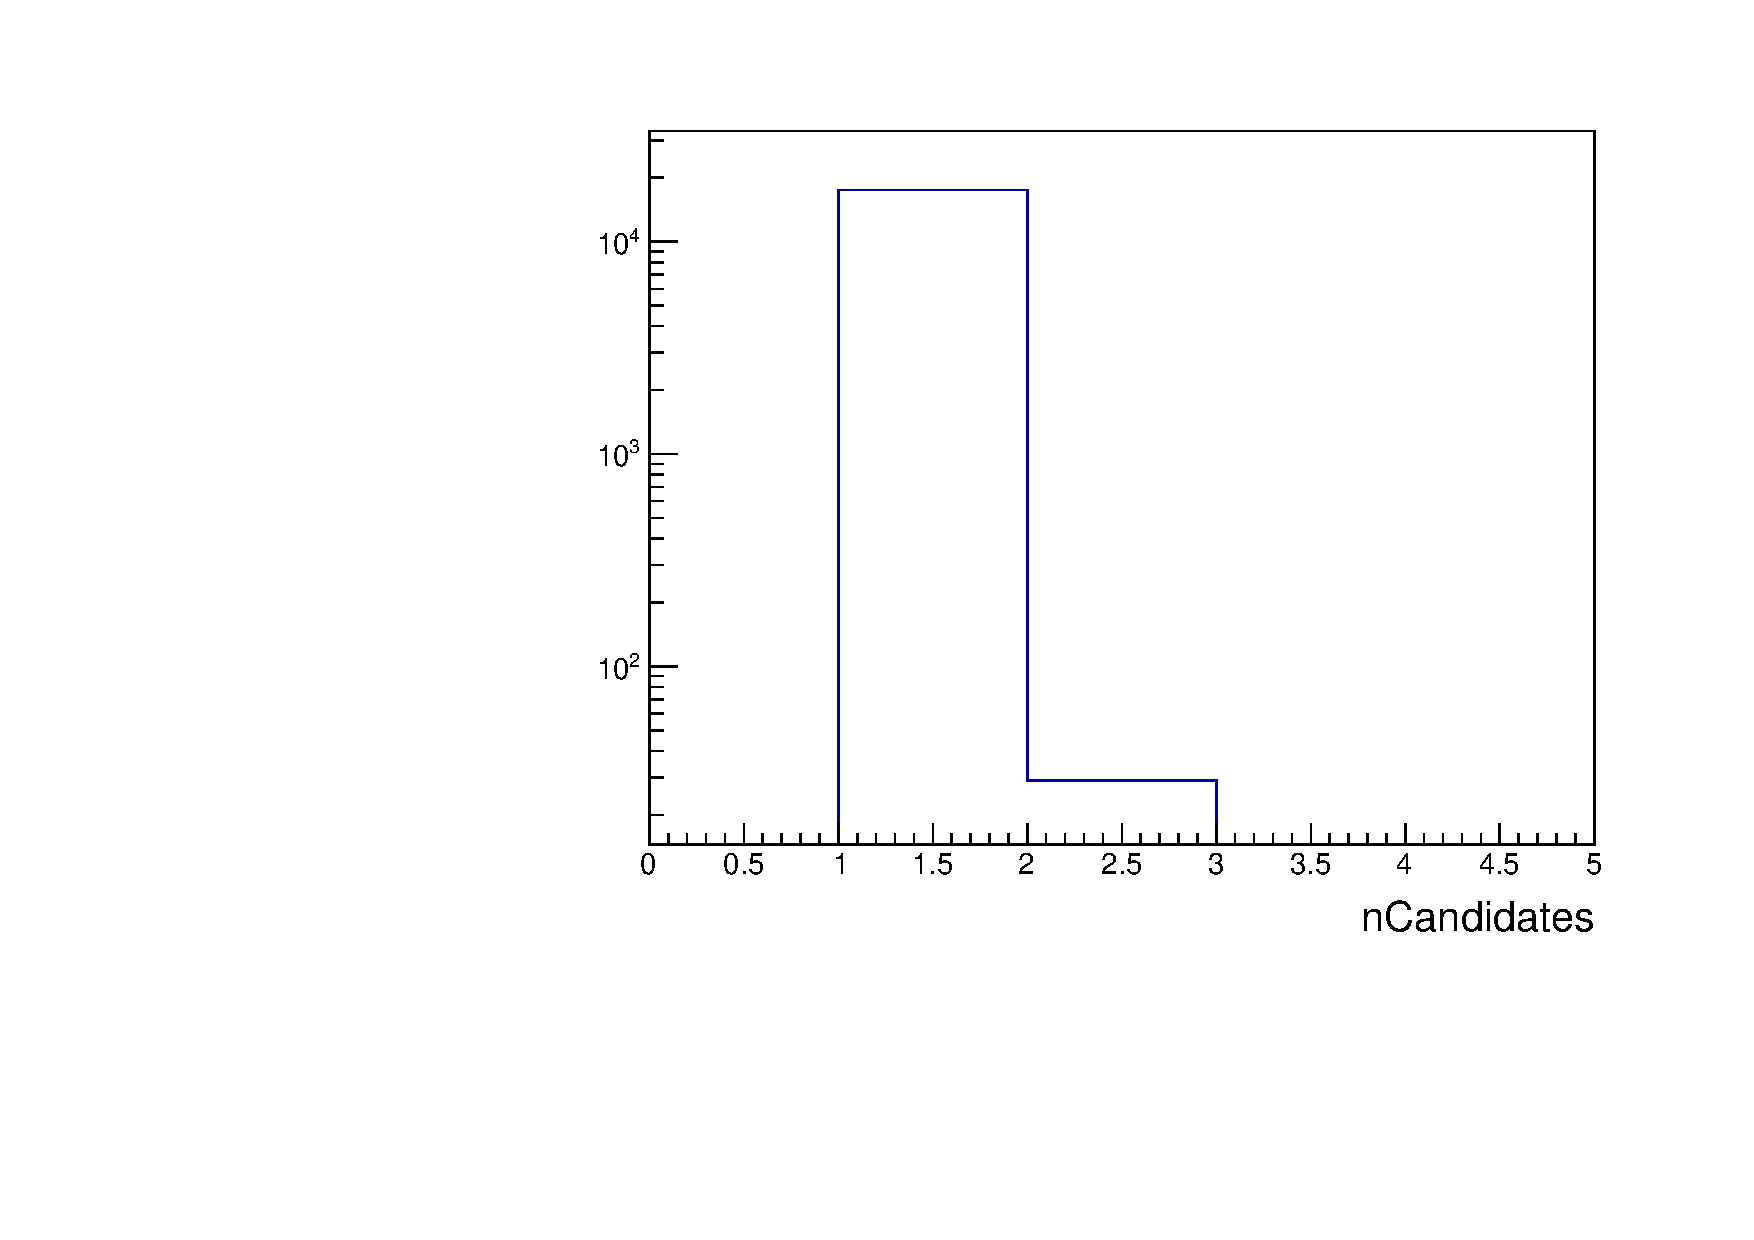
\includegraphics[width=\textwidth]{Cuts/nCandM.pdf}
	\end{minipage}
	\hspace{0.5cm}
	\begin{minipage}[b]{0.45\linewidth}
		\centering
		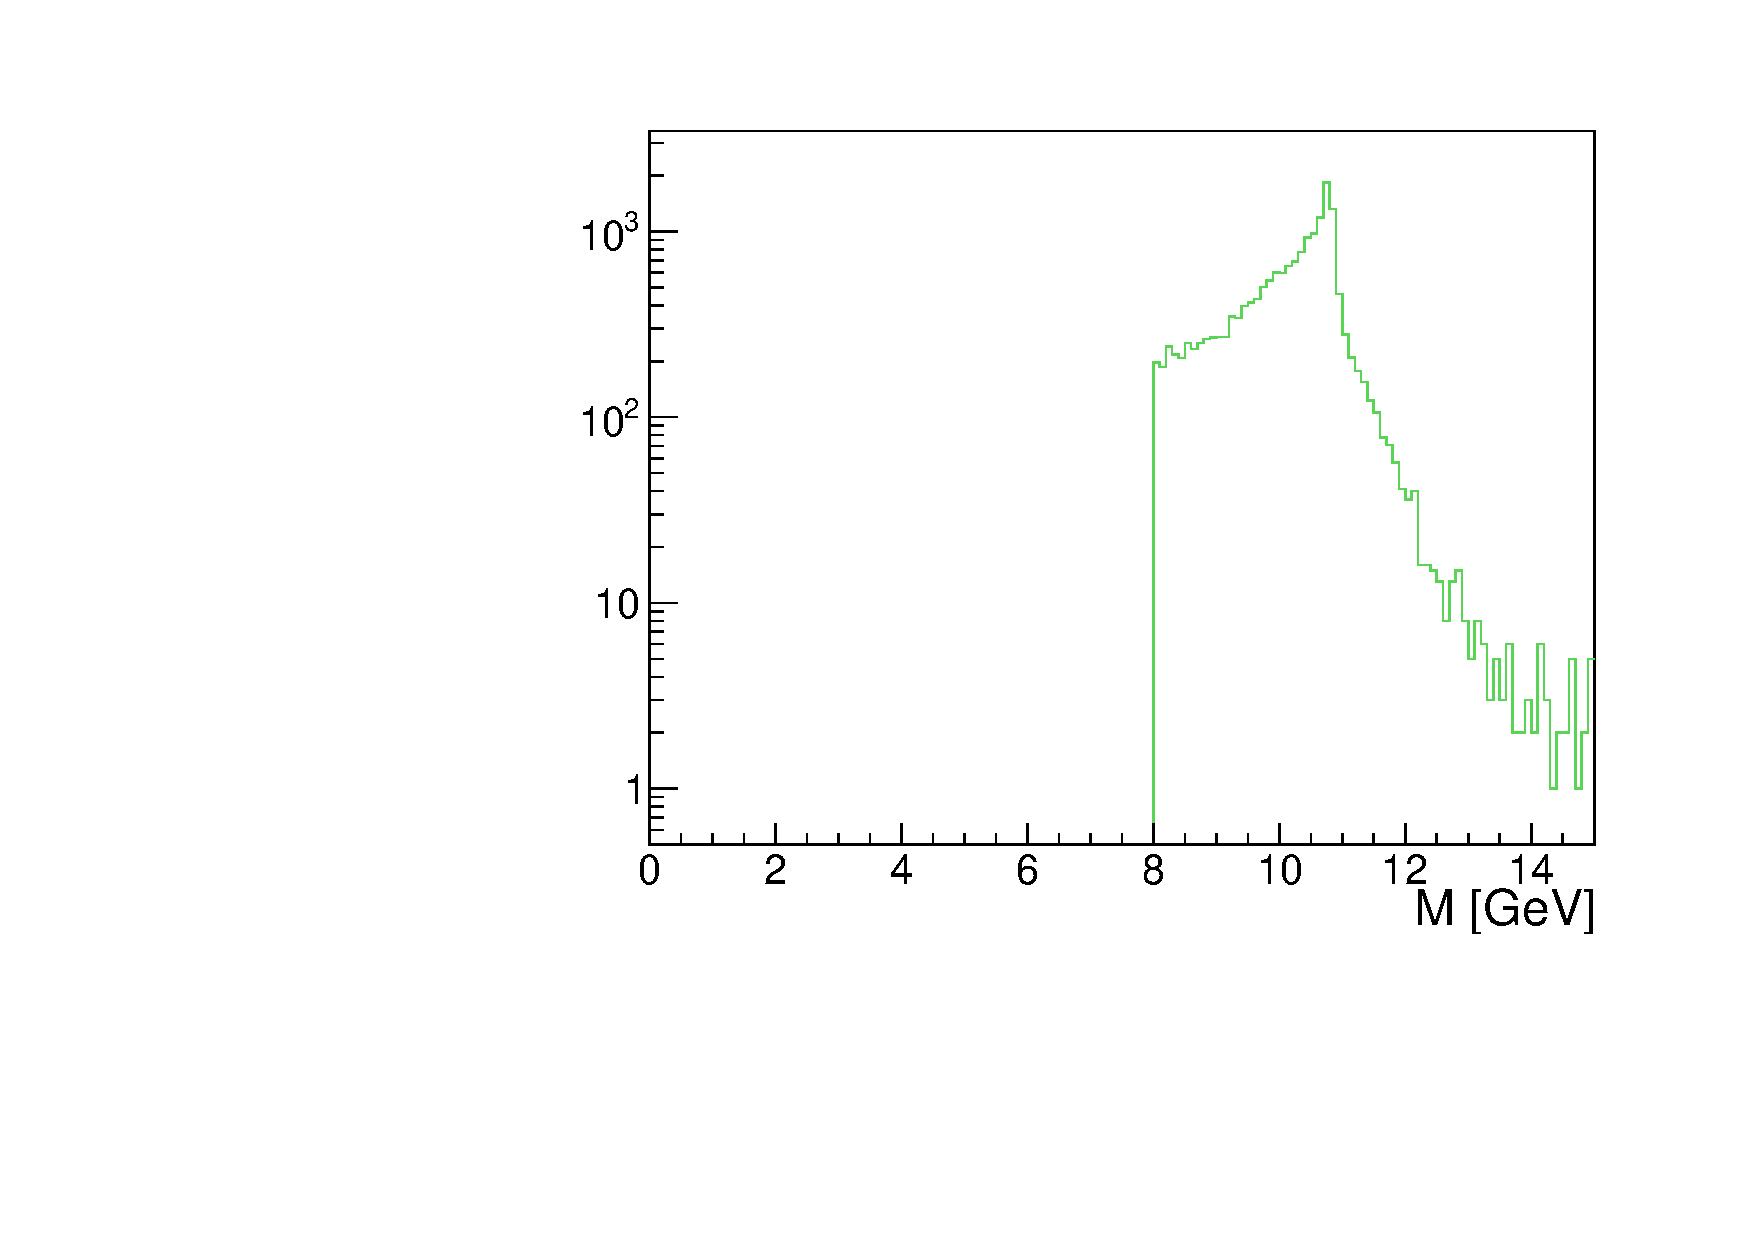
\includegraphics[width=\textwidth]{Cuts/MM.pdf}
	\end{minipage}
	\caption[Number Of Candidates And Invariant Mass ($\textrm{M} >8\,\textrm{GeV}$)]{A cut on the invariant mass is applied. The reconstructed invariant mass has to be bigger than $8\,\textrm{GeV}$. Left: The number of reconstructed candidates per event is shown. We select 17539 events. Right: The invariant mass of the reconstructed candidates is shown. We select 17558 candidates.}
	\label{fig:nCandM}
\end{figure}

As you can see in figure \ref{fig:nCandM} on the right, all reconstructed candidates with an invariant mass below $8\,\textrm{GeV}$ are neglected. Therefore, the number of candidates per event is reduced. We see this in the left plot. Unfortunately, sometimes we still have two candidates per event and consequently, we have to introduce some more additional cuts.



\subsection{Additional Cuts}

To reduce the number of candidates per event to one, some additional cuts are needed. Sometimes it can happen that two reconstructed particles are associated to one Monte Carlo particle. Some examples of this effect can be seen in table \ref{tab:clusterSplitting}. 


\begin{table}[h!]
	\centering
	\makebox[\textwidth]{
		
		\begin{tabular}{l|cccc|cccc}
			& \multicolumn{4}{c|}{HclE} & \multicolumn{4}{c}{LclE}\\
			\cline{2-9}
			
			Event Number& E &mcE&PDG&mcPDG & E&mcE&PDG&mcPDG  \\
			\hline
			41890065&0.9432 & 4.1278& 11&11& 3.1900&4.1278 & 22&-11 \\
			41890118&1.5993 &4.3465 &22 &11& 2.6462& 4.3465&-11 &-11 \\
			41890668&3.1758 &6.8878 &22 &-11&3.1059 &6.8878 &11 &11 \\
			41891214 &2.3290 & 6.1585&22 &-11& 3.9079&6.1585 &11&11  \\
			41892596 &1.4193 & 4.2997& 22&11&2.9673 &4.2997 &-11 &-11 \\
		\end{tabular}
	}
	\caption[Cluster Splitting Examples]{Some examples for events with cluster splitting. mcE is the same for LclE and HclE. The energies are in GeV. }
	\label{tab:clusterSplitting}
\end{table}




As you can see, the Monte Carlo generated energy (mcE) for both HclE and LclE is the same and the reconstructed energy (E) of the HclE and the LclE particle sum up roughly to their respectively mcE. You can also see that the generated particle is always an electron or positron and that the \textit{additionally} reconstructed particle is always a photon.







In figure \ref{fig:clusterSplittingAngle} you can see the angular distribution of this effect. For this plot there were no cuts on the reconstruction. It was just checked if exactly two reconstructed particles have the same generated Monte Carlo particle associated. Then the clusterPhi- and clusterTheta-values of these particles were filled into their histograms. On the left, you can see that both reconstructed particle have the same clusterTheta angle. On the right you can see that they have a slightly different clusterPhi angle. Therefore, the one \textit{original} cluster  is separated into two clusters with the same $\theta$-angle and a different $\Phi$-angle. One cluster is associated with a track produced by the generated particle and for the other cluster no track is left, therefore, it is labeled as a photon. This effect will be referred to as \textit{cluster splitting}.





\begin{figure}[h!]
	\centering
	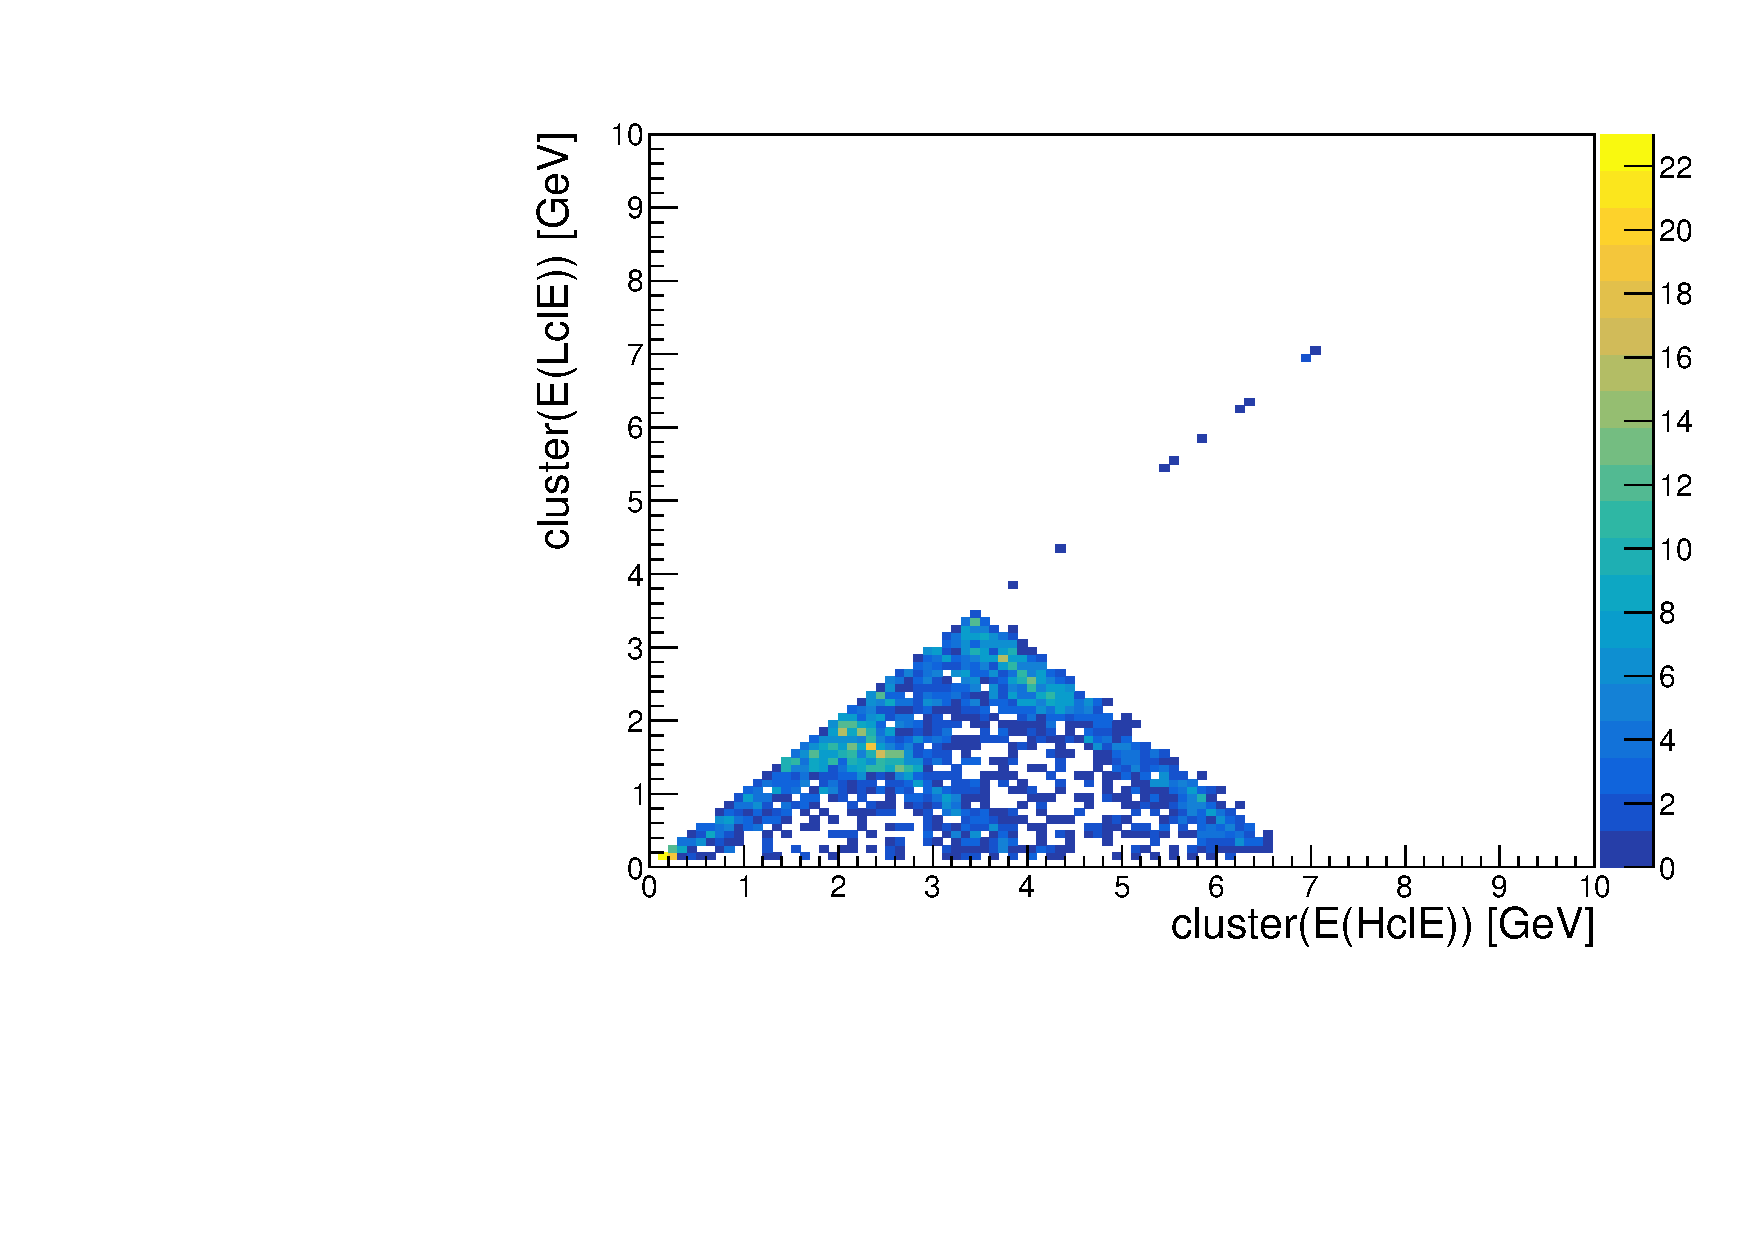
\includegraphics[width=10cm]{AnhangPlots/EEdoubleMCE}
	\caption[Cluster Splitting Energy Distribution]{Cluster Energy vs. Cluster Energy in the case that both particles are associated to the same Monte Carlo particle. Here, no cuts are applied. The total number of entries is 2891.}
	\label{fig:clusterSplittingE}
\end{figure}

In figure \ref{fig:clusterSplittingE} you can see the energy of the particles in a cluster splitting process. Since we only want to select Bhabha events, we want to neglect these kinds of events. In section \ref{sec:Kinematics} we saw that the particles have an energy of at least $4\,\textrm{GeV}$. Therefore we are able to apply a cut on the cluster energy. We are now requiring a cluster energy of at least $3.5\,\textrm{GeV}$ (The cut is called \texttt{MclE}). With this cut almost all events with cluster splitting should be neglected.

Next, we require that we have exactly two clusters per event, each with an energy of at least $3.5\,\textrm{GeV}$, since we only expect two high energetic particles in the ECL. Also, due to the kinematics at Belle II, we can require that one of the outgoing particles has an cluster energy of at least $4.5\,\textrm{GeV}$. This is required due to the trigger we will add in section \ref{sec:ECLTrigger}. (the cut is called \texttt{MclE2H}).

As an additional safety net, a cut on the number of reconstructed tracks per event is applied. On data it can happen that there are way more than two tracks reconstructed per event. To select only \textit{clean} events we apply a cut on the number of reconstructed charged particles per event (The cut is called \texttt{MclE2HnT}). This number should not be greater than six.


\begin{table}[h!]
	\centering
	\begin{tabular}{lcccc}
		
 Event Number&M &Energy(\texttt{HclE}) &Energy(\texttt{LclE}) &Total Energy ECL \\
 \hline
 
41890917 & 30.6657& 33.8368& 7.2455& 41.0823\\


26574414 & 108.4056 & 235.3918 &13.0644 &  248.4563\\

21222871 &11.6553 & 2.1733& 15.6648& 17.8381\\

26372406 & 10.3229& 0.2465&190.2663 & 194.5971\\
	\end{tabular}
\caption[Energy Sum In The ECL Examples]{Some examples for events with too much energy in the ECL. 
	
	Note: Here the energy of the particles is shown not clusterE.}
\label{tab:ESum}
\end{table}

As you can see in table \ref{tab:ESum}, sometimes the invariant mass of the reconstructed candidates is way bigger than $10.58\,\textrm{GeV}$. To neglect these candidates an upper cut on the reconstructed invariant mass is introduced. Now, the reconstructed invariant mass also has to be smaller than $12\,\textrm{GeV}$.

Also, sometimes the total energy in the ECL is way higher than expected. To exclude these events an upper cut on the total energy per event in the ECL is added (The cut is called \texttt{MclE2HnTSumE}). The total energy in the ECL must not exceed $15\,\textrm{GeV}$.



\begin{figure}[h!]
	\centering
	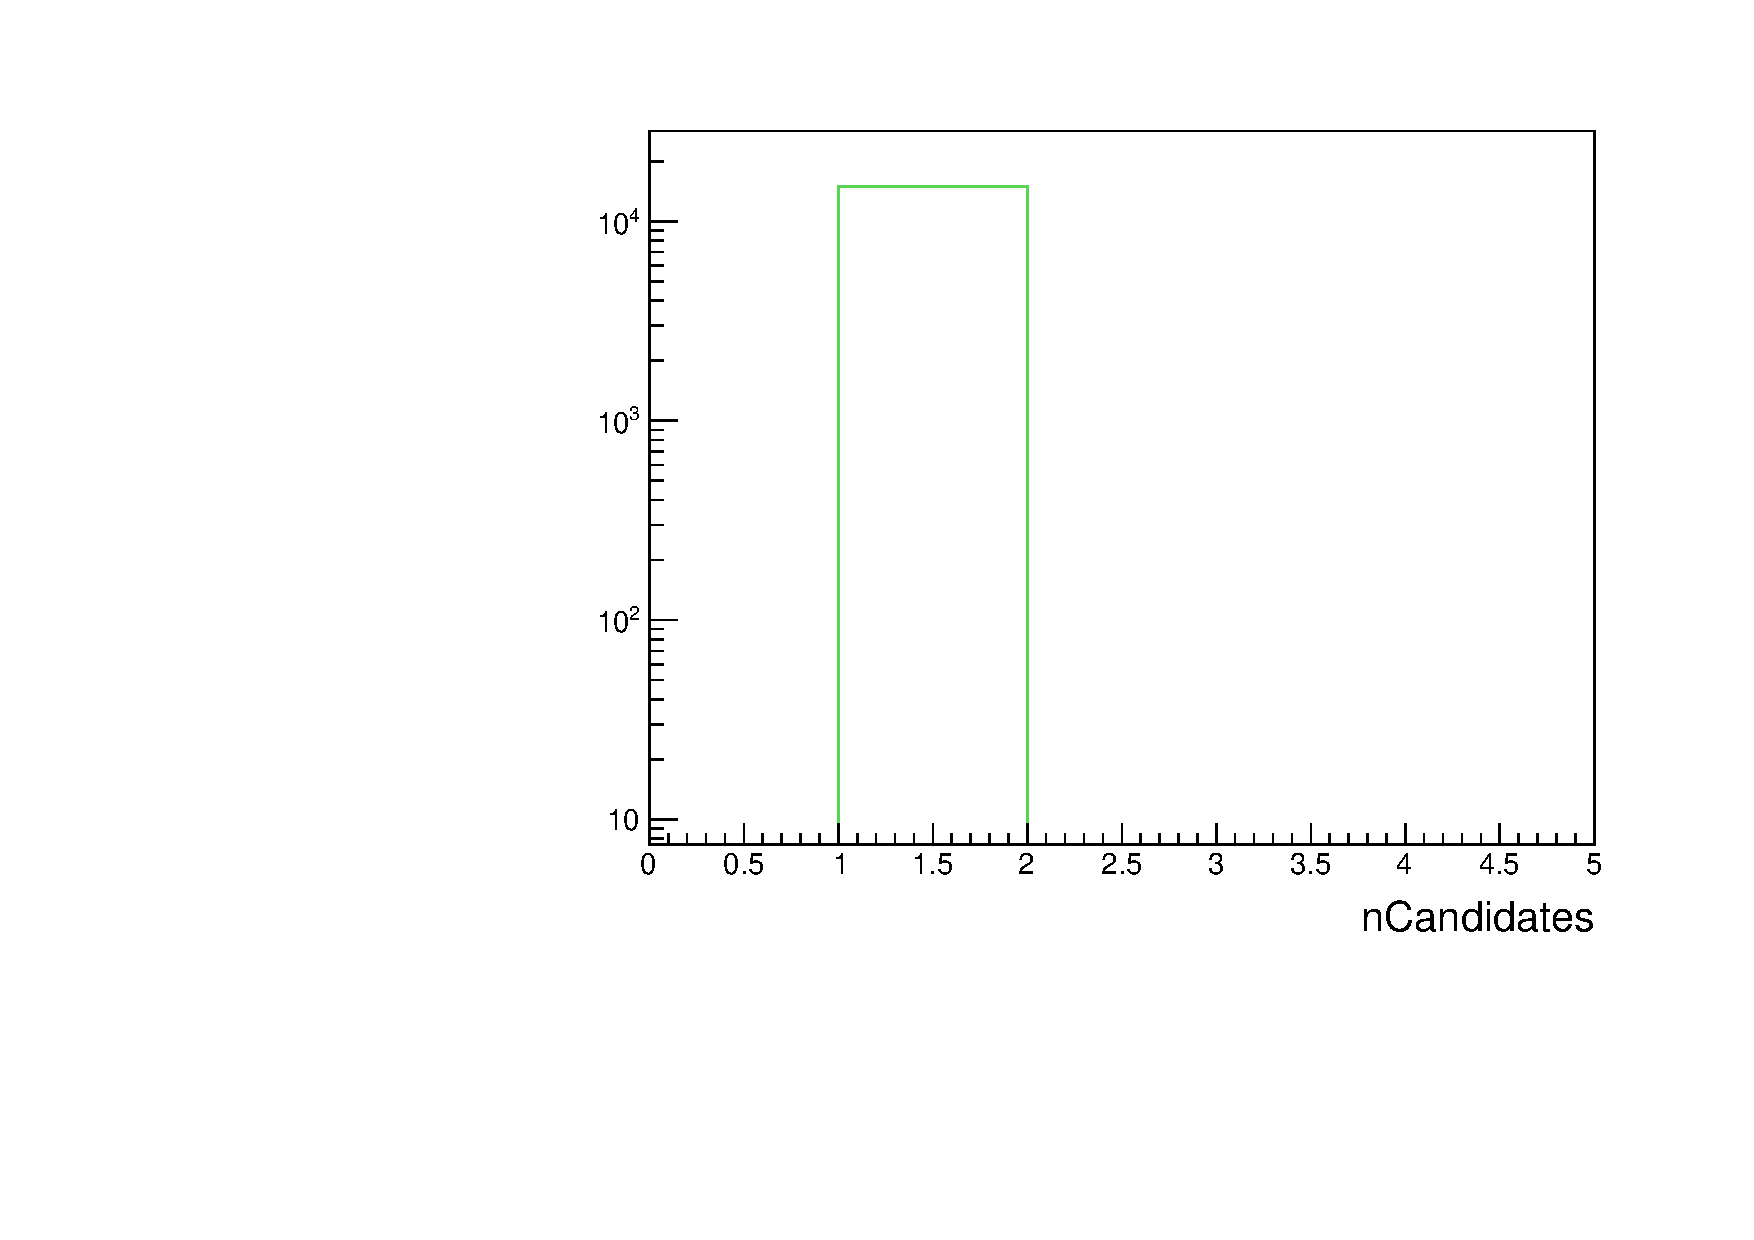
\includegraphics[width=10cm]{Cuts/nCand.pdf}
	\caption[Number Of Candidates Per Event (All Cuts)]{Number of candidates per event after applying all cuts. $n = 14545$}	
	\label{fig:nCand}
\end{figure}

After applying all mentioned cuts, the number of candidates per event is shown in figure \ref{fig:nCand}. As you can see, now, we only select one candidate per event. Therefore, we select 14545 events and candidates.

There is no cut on the interaction point since this would require a backtracking of the particles.




\subsection{Cut Efficiency}

In this section we want to discuss different efficiencies of the previously introduced cuts. We will take a look at the relative and the total efficiency. The results can be seen in table \ref{tab:cutEff}.

\begin{equation}
	\epsilon_{\textrm{tot}} = \frac{n_{\textrm{cut}}}{n_{\textrm{total}}}
	\label{eq:cutTotEff}
\end{equation}

To calculate the total efficiency of a cut we have to use equation \ref{eq:cutTotEff}. Here the number of events after a cut $n_{\textrm{cut}}$ is divided by the total number of events $n_{\textrm{total}}$ before all cuts\footnote{The cut that requires that the generated particles have to pass the CDC is still applied $\rightarrow n_{\textrm{total}} = 24100$}.

\begin{equation}
	\epsilon_{\textrm{rel; Cut B}} = \frac{n_{\textrm{Cut B}}}{n_{\textrm{Cut A}}}
	\label{eq:cutRelEff}
\end{equation}

Equation \ref{eq:cutRelEff} shows the equation used to calculate the relative efficiency. To calculate the efficiency of cut B we have to divide the number of events after cut B by the number of events after the previous
cut A. The relative efficiency with no cut is defined as 1.

\begin{table}[h!]
	\centering
\begin{tabular}{lccc}
 Cut& Number Of Events&  Relative Efficiency& Total Efficiency\\
 \hline
 No Cut&24100 &1.0000 &1.0000 \\
 \texttt{M}& 17529&0.7273 &0.7273 \\
 \texttt{MclE}&14903 &0.8502 &0.6183 \\
 \texttt{MclE2H}&14896&0.9995  &0.6180 \\
 \texttt{MclE2HnT}&14896 &1.0000 &0.6180 \\
 \texttt{MclE2HnTSumE}& 14545 &0.9764 &0.6035 \\

\end{tabular}

\caption[Cut Efficiencies]{A table with the total number of events after the respective cuts. Also the relative and the total efficiency of these cuts is shown. The total number of entries in the \textit{mcEvtCDC}-list is 24286.}
\label{tab:cutEff}
\end{table}

Table \ref{tab:cutEff} shows the relative and total efficiency of the cuts.
As you can see, after all cuts a total of about $62\%$ generated Bhabha events are reconstructed. 

\subsection{No MC-Truth Information}
\label{sec:NoMCT}

In the previous sections we saw that we are able to select only one candidate in a Bhabha event under the condition that we know that both daughters are hitting the ECL. Unfortunately, we do not have this information on phase2 data. Therefore, we also check how many candidates we reconstruct if we do not have MC-Truth information. We will analyze the same MC-file as before to compare the number of reconstructed events. 


\begin{figure}[h!]
	\centering
	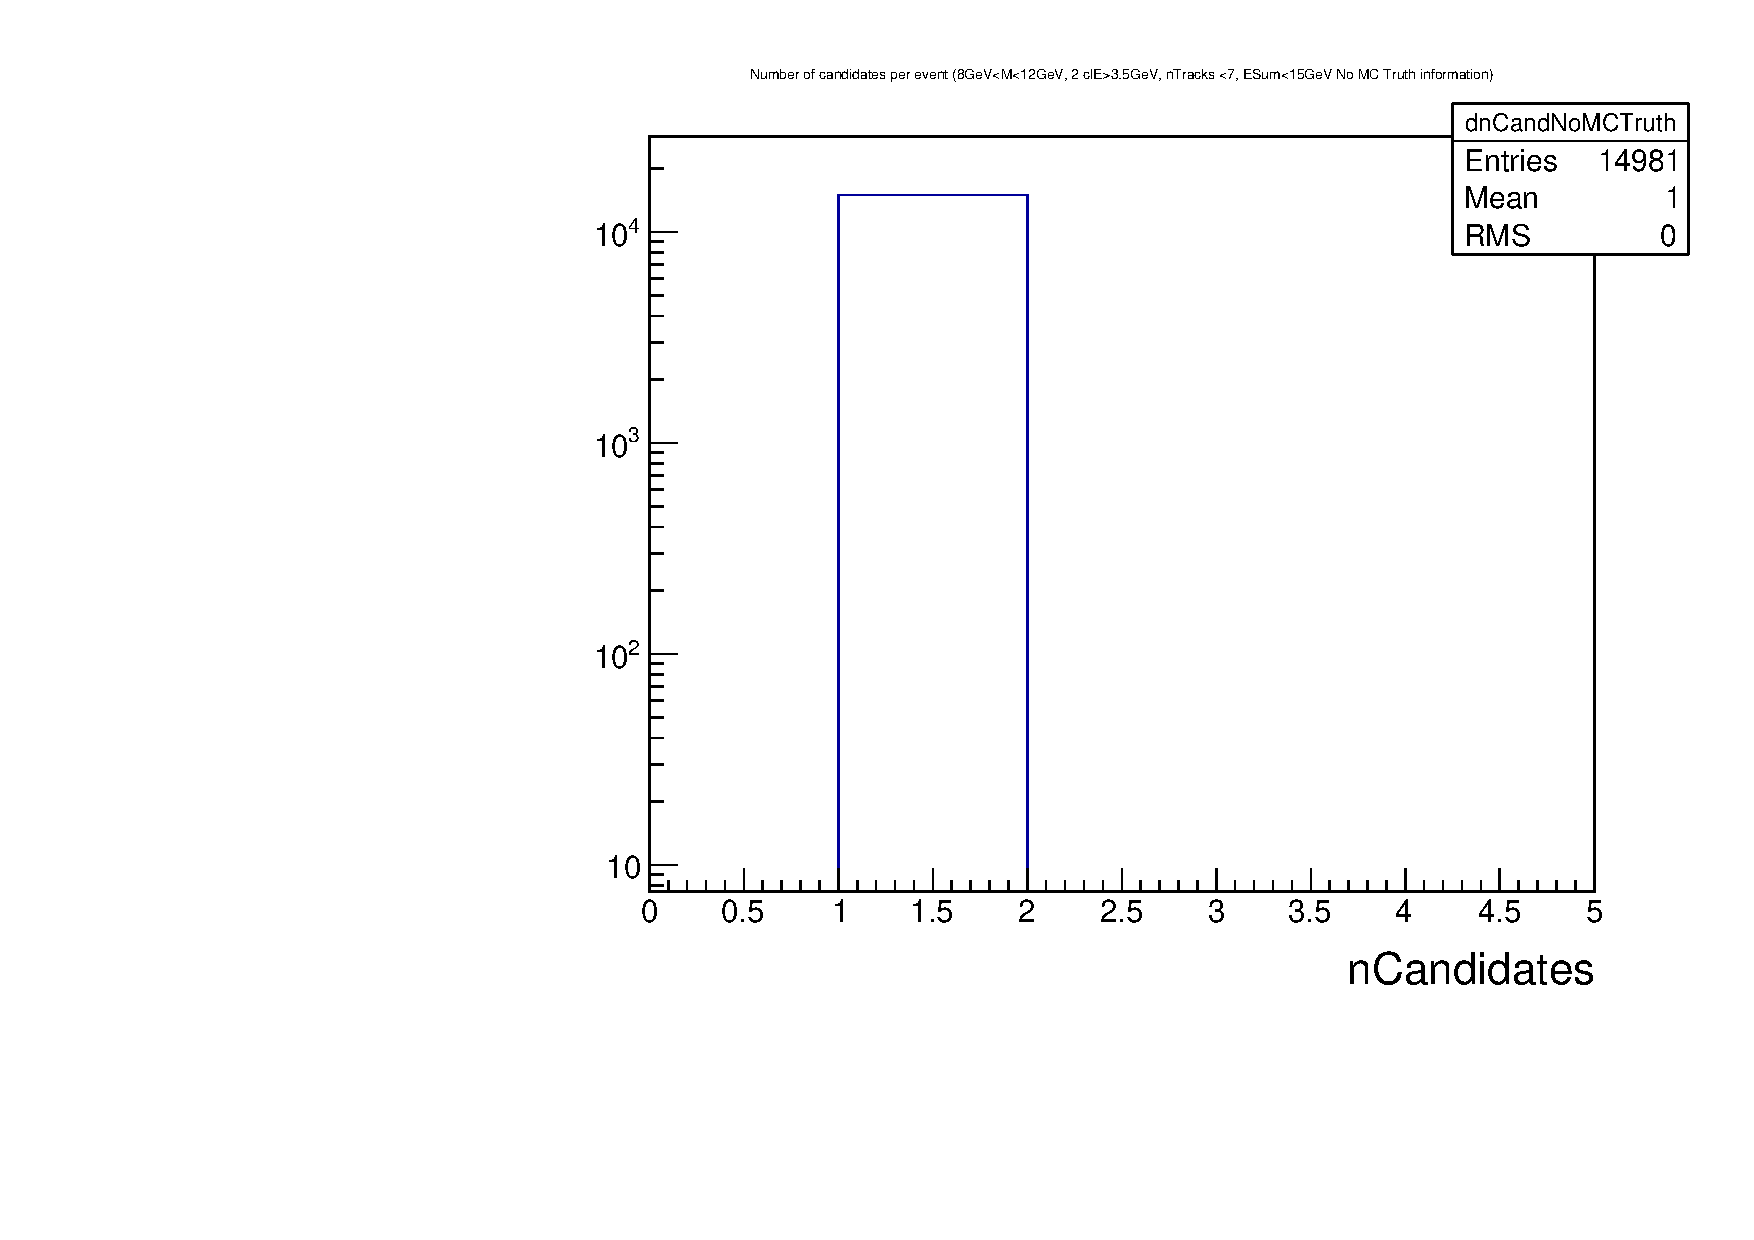
\includegraphics[width=10cm]{Cuts/nCandNoMCInfo.pdf}
	\caption[Number Of Candidates Per Event With No MC-Truth Info (All Cuts)]{Number of candidates per events with no MC-Truth information and all cuts. Same MC file as before. We also select just one candidate per event. The total number of selected events is 14581.}
	\label{fig:nCandNoMCInfo}
\end{figure}

In figure \ref{fig:nCandNoMCInfo} we see that we reconstruct a total number of 14581 events. Therefore, we reconstruct only 36 events more with no MC-Truth information. Also, we are still able to select only one candidate per event. 

Since we only reconstruct a few more events and still only one candidate per event, we can be very confidant that we only select almost exclusively Bhabha events.

\section{Best Candidate Selection on Phase2 Data}
\label{sec:SelectingBhabhaData}

Until now we only ran on MC, but ultimately we want to calculate the tracking efficiency on phase2 data. Therefore, we have to test the selection also on phase2 data. The same steering file as described in section \ref{sec:RecBasf2} is used and run over the following files located at:


/ghi/fs01/belle2/bdata//Data/release-03-00-03/DB00000528/proc00000008/e0003/
4S/r02608/all/mdst/sub00/*.root


The generated file is located on KEKCC at:

/home/belle2/msobotzi/bhabha/bhabha\_vpho\_data\_608.root

\begin{figure}[h!]
	\centering
	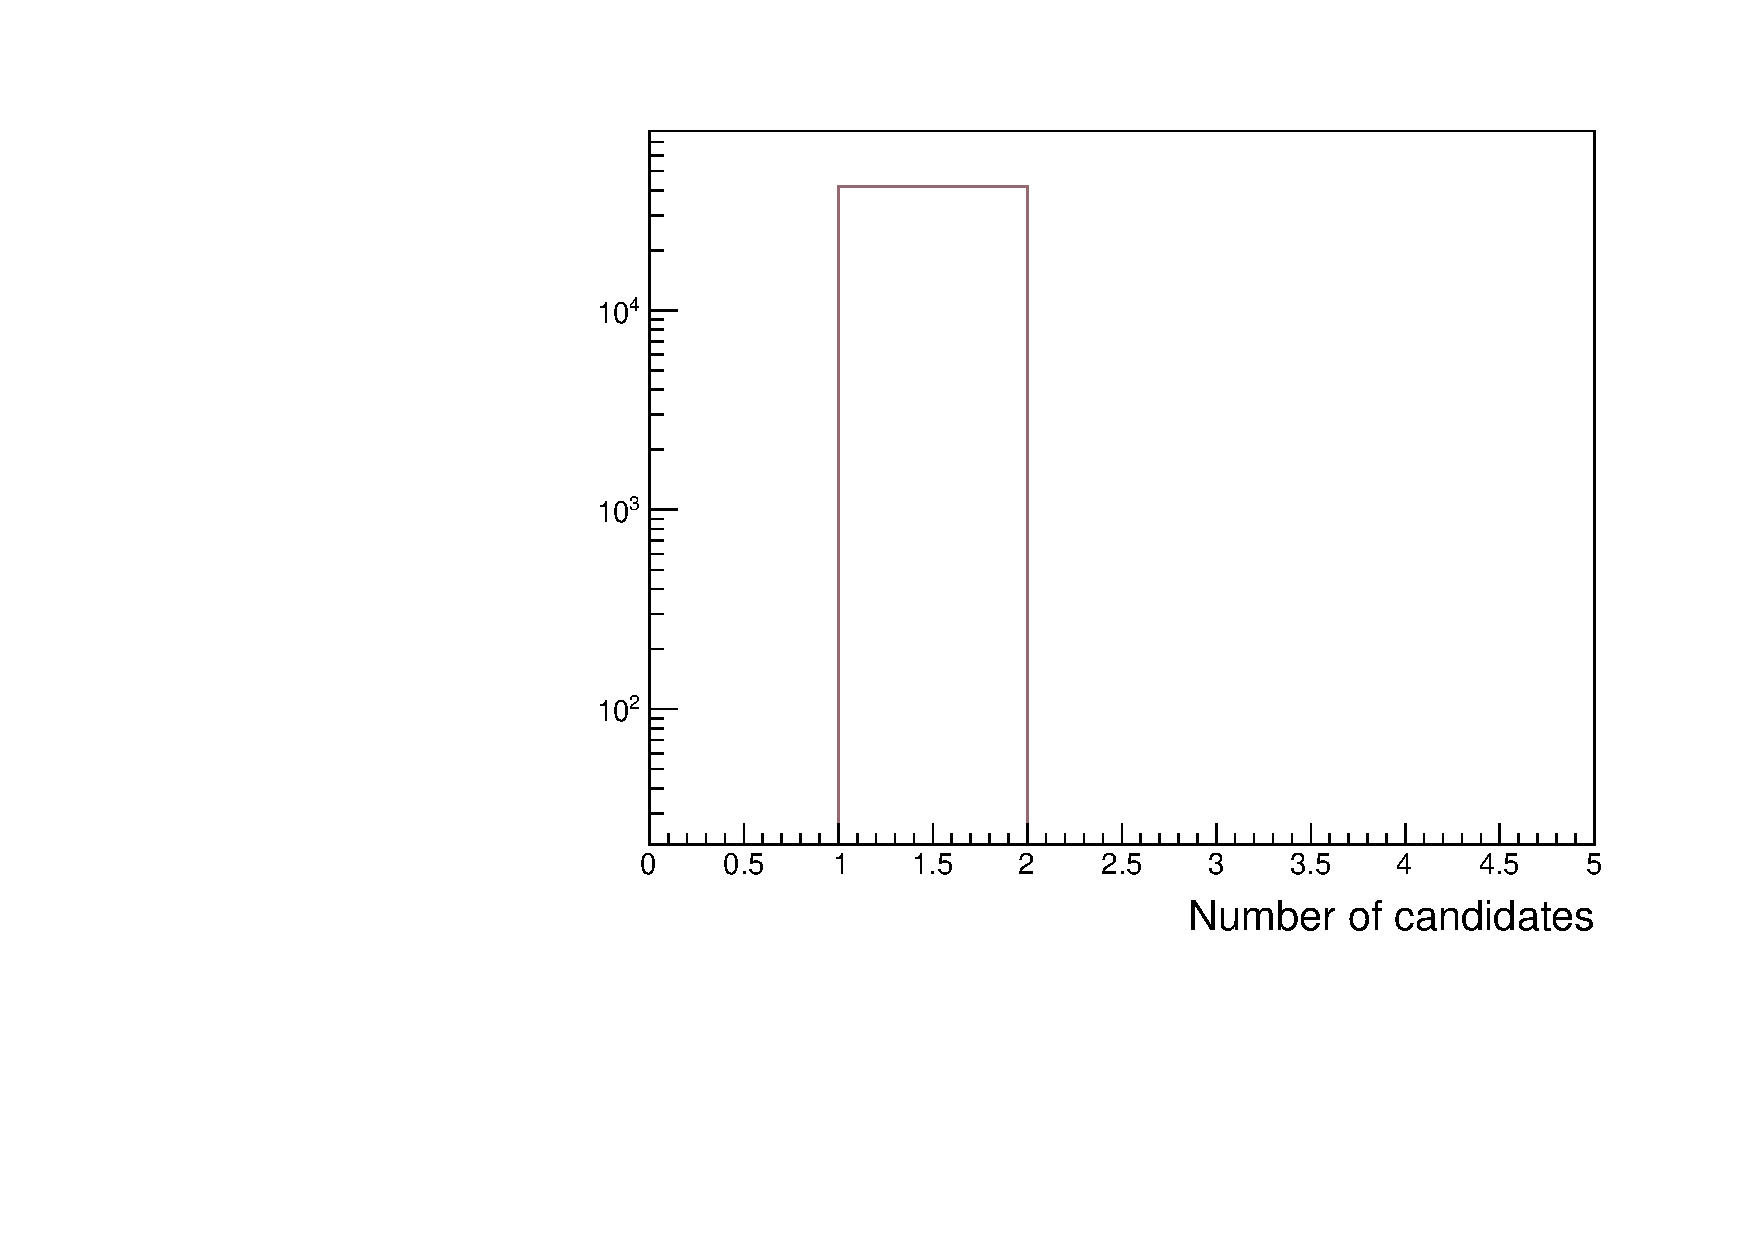
\includegraphics[width=10cm]{Cuts/Data/nCandData.pdf}
	\caption[Number Of Candidates Per Event for Phase2 Data (All Cuts)]{Number of candidates per event for phase2 data. We also select only one candidate per event on phase2 data. A total number of 41853 events and candidates is selected.}
	\label{fig:nCandData}
\end{figure}

Figure \ref{fig:nCandData} shows the number of reconstructed candidates on phase2 data after the \texttt{MclE2HnTSumE} cut. You can see that we reconstruct only one candidate per event even on phase2 data.



\section{Selecting Bhabha Events}
\label{sec:SelectingElectronPositron}

Now, that we are satisfied with the selection of events and candidates we need to be sure that we only select $\textrm{ee} \rightarrow \textrm{ee}$ events and not for example $\textrm{ee} \rightarrow \gamma \gamma$. This is important on phase2 data since there are no $\textrm{ee} \rightarrow \gamma \gamma$ events on Monte Carlo. To do this we can use the so-called b2b-variable (back-to-back).

\begin{figure}[h!]
	\centering
	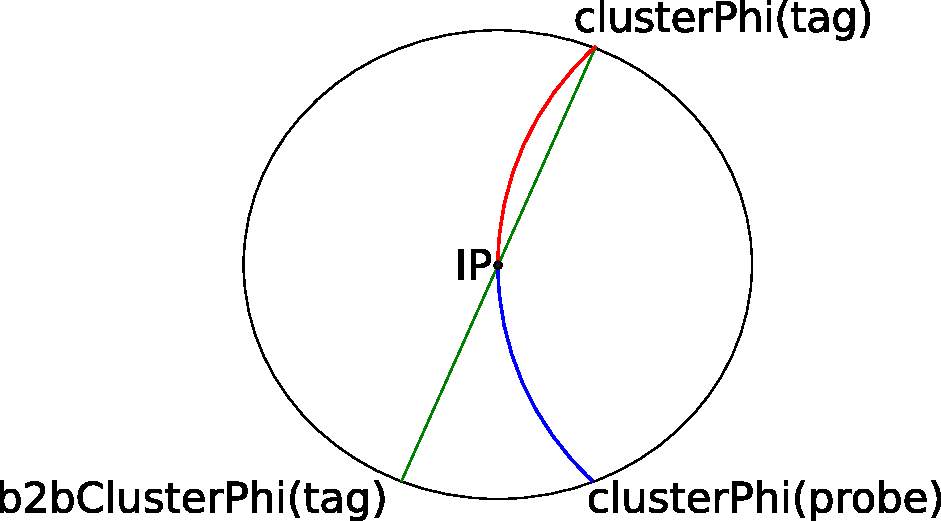
\includegraphics[width=10cm]{Bilder/b2b_2}
	\caption[Sketch Of The b2bClusterPhi Variable]{Simplified representation of the b2bClusterPhi variable. The track of charged particles are bend in the detector. This sketch was created with Inkscape. The colors have no deeper meaning.}
	\label{fig:Sketchb2b}
\end{figure}

A simplified sketch of the b2bClusterPhi variable is shown in figure \ref{fig:Sketchb2b}. This sketch shows the ECL in beam direction, so the magnetic field in the ECL is pointing into the paper. At the interaction point an electron (in this example the red line) and a positron (in this example the blue line) are created. Since both particles are charge their trajectory is bended by the magnetic field. The electron hits the ECL and creates a cluster with at the $\phi$-angle clusterPhi. As described in section \ref{sec:Kinematics} the center-of-momentum frame at Belle II has a non zero $x-y$ fraction. Therefore, the b2bClusterPhi variable is not just $\textrm{clusterPhi} - \pi$ (as in the sketch). To calculate the b2bClusterPhi variable we have to boost the particle in the center-of-momentum frame then calculate $\textrm{clusterPhi} - \pi$ and finally boost back in the lab frame. With this variable we can predict the clusterPhi angle of the other particle. 

In the sketch you see that there is a difference between the predicted and the true clusterPhi angle due to the magnetic field. This also means that in an $\textrm{ee} \rightarrow \gamma \gamma$ event the predicted and the true clusterPhi angle are the same because the trajectory of photons are not bend in the magnetic field. Therefore, we are able to differ between $\textrm{ee} \rightarrow \textrm{ee}$ and $\textrm{ee} \rightarrow \gamma \gamma$.



\begin{figure}[h!]
	

\begin{minipage}[b]{\textwidth}
\centering


	\begin{minipage}[b]{0.45\linewidth}
		\centering
		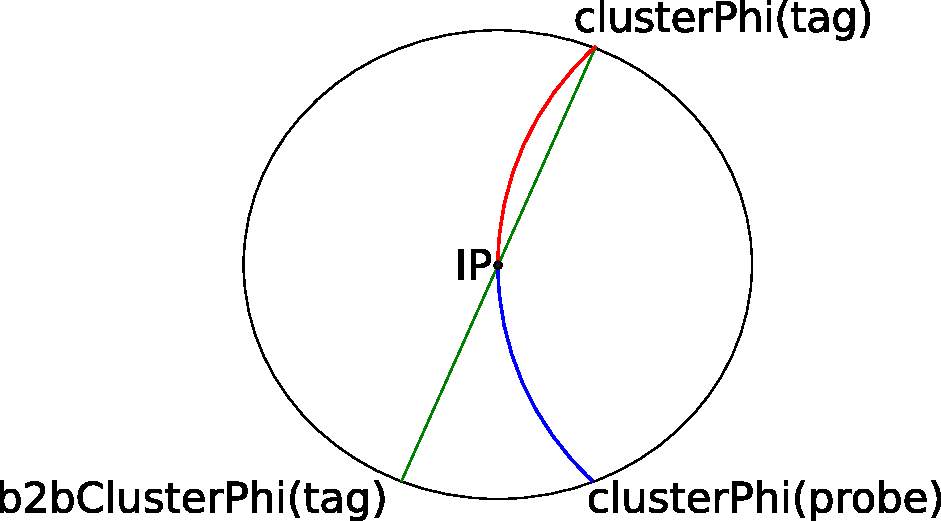
\includegraphics[width=\textwidth]{Bilder/b2b_2}

	\end{minipage}
	\hspace{0.5cm}
	\begin{minipage}[b]{0.45\linewidth}
		\centering
		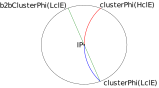
\includegraphics[width=\textwidth]{Bilder/b2b_3}
	\end{minipage}
	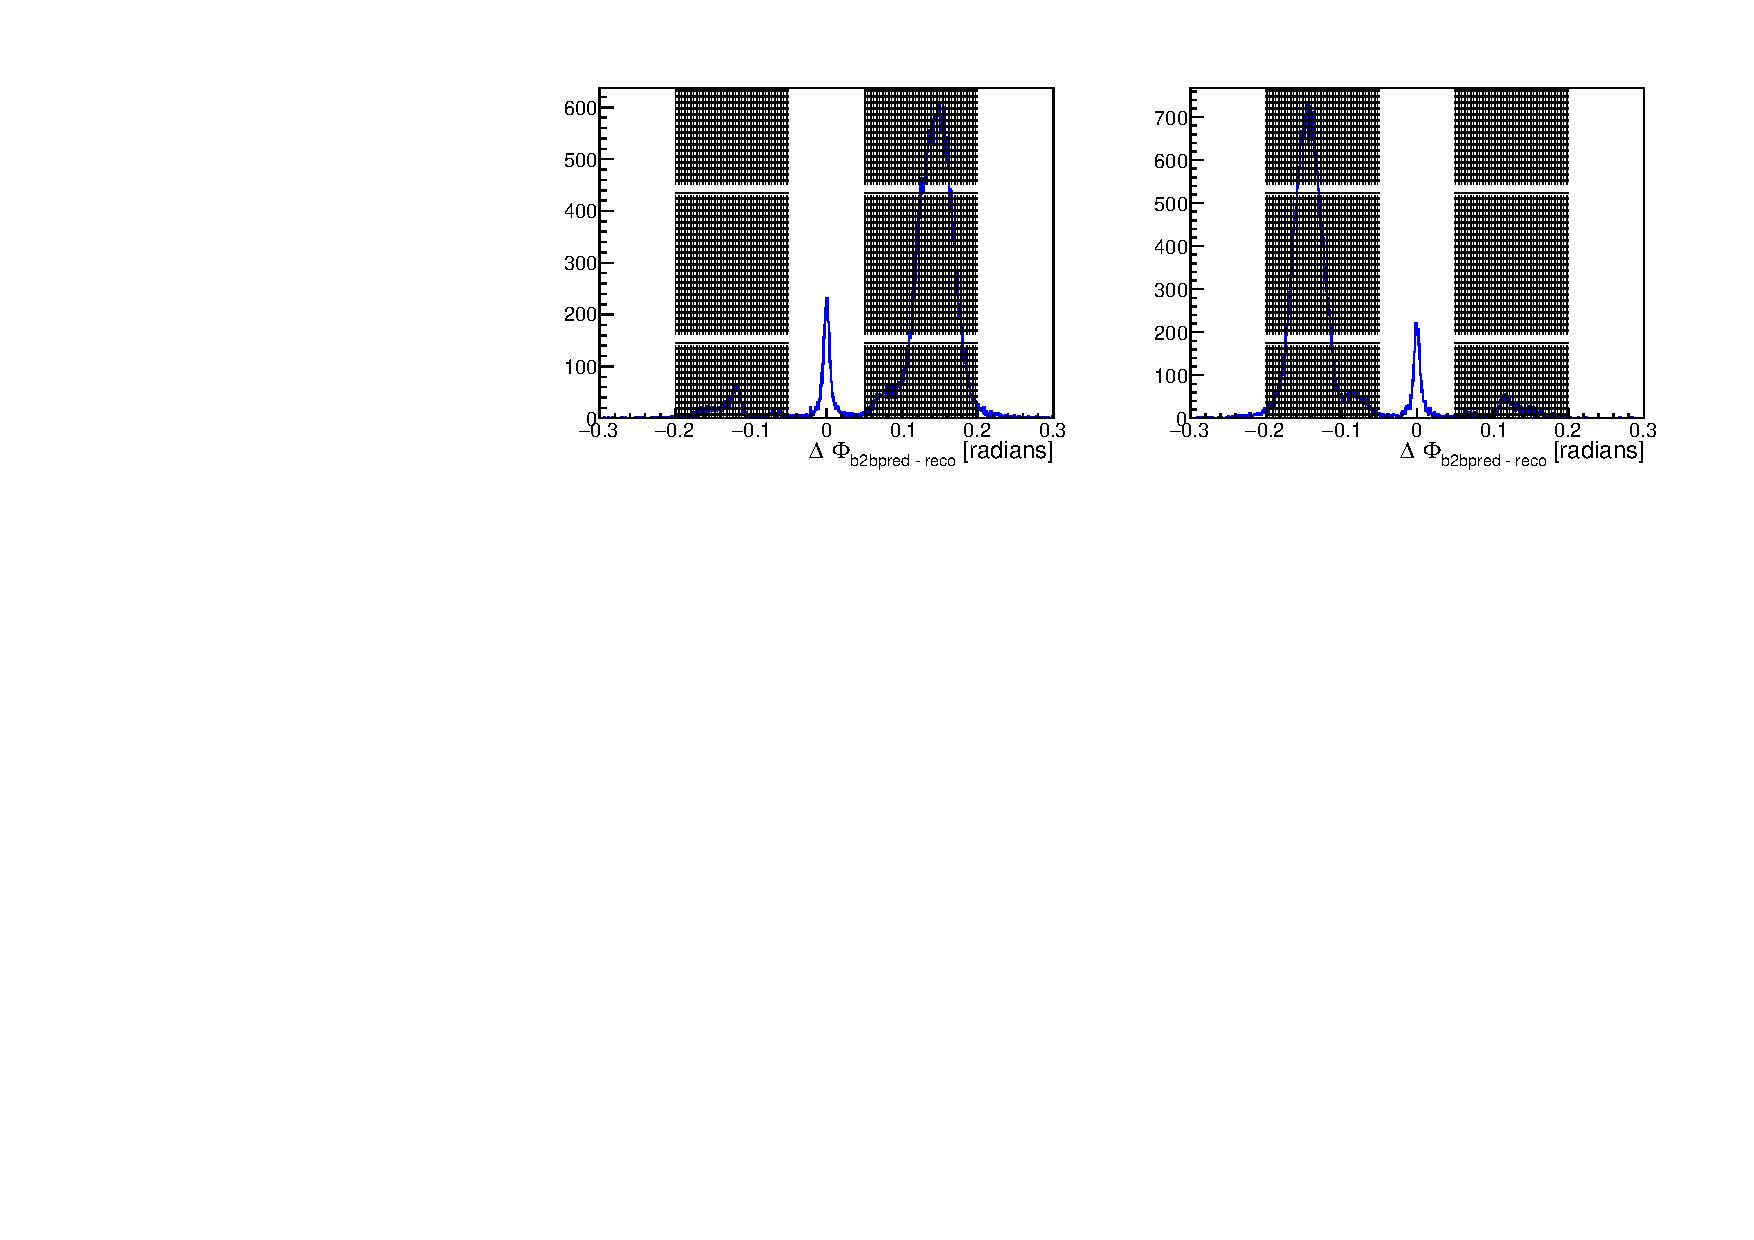
\includegraphics[width=\textwidth]{Plots/master/sb2b_Data.pdf}
	

	\caption[b2bClusterPhi - clusterPhi For Beamtime-Data]{Left: Predicted clusterPhi(HclE) - Reconstructed clusterPhi(LclE). Right: Predicted clusterPhi(LclE) - Reconstructed clusterPhi(HclE). Only particles within the gray area are taken into account. Both plots are created with phase2 data. The variable to get the predicted clusterPhi value is the b2bclusterPhi variable which was described earlier. The two top sketches represent what is calculated.}
	\label{fig:b2bData}
	%Single Data file 608 Efficiency.C makro

\end{minipage}
\end{figure}


In figure \ref{fig:b2bData} the difference between the predicted and the reconstructed clusterPhi angle for phase2 data is shown. In the left plot the reconstructed clusterPhi angle of the LclE particle is subtracted by the b2bClusterPhi angle of the HclE particle. In the right plot it is vice versa. In both plots we have three peaks. The middle peaks are $\textrm{ee} \rightarrow \gamma \gamma$ events since the predicted and the reconstructed clusterPhi angle is the same. So these are events we want to cut away. The left peak is caused by electrons (most of the HclE particles are electrons, therefore the left peak on the right plot is significantly higher\footnote{As described in section \ref{sec:RecBasf2}, the HclE daughter is the daughter with the higher cluster energy}), the right peak by positrons. This means that if for example we only cut on the left peak we are only selecting electron particles even if they are wrongly reconstructed as photons, using ECL information only. 
Therefore, the last cut we will add is a cut on the b2bClusterPhi angle. We will only consider events in with:
\newline

 $0.05 \leq \textrm{abs(b2bClusterPhi(HclE) - clusterPhi(LclE)} \leq 0.2 $ and  $0.05 \leq \textrm{abs(b2bClusterPhi(LclE) - clusterPhi(HclE))} \leq 0.2$
\newline



A special case occurs for $\Phi \approx \pi$ or $\Phi \approx -\pi$. It can happen that the reconstructed clusterPhi angle is around $\pi$ but the b2bClusterPhi angle is calculated to be around $-\pi$, then the difference between the predicted and reconstructed clusterPhi angle is around $2\pi$. This can be seen in figure \ref{fig:b2bData_Whole}

Finally, the b2bClusterPhi variable cut can be summarized in the following three conditions. Each event has to fulfill one of them to be taken into account.

\begin{enumerate}[label=(\alph*)]
	\item $0.05 \leq \textrm{abs(b2bClusterPhi(HclE) - clusterPhi(LclE)} \leq 0.2 \, \&\& \, 0.05 \leq \textrm{abs(b2bClusterPhi(LclE) - clusterPhi(HclE))} \leq 0.2$
	\item $2\pi - 0.2 \leq \textrm{abs(b2bClusterPhi(HclE) - clusterPhi(LclE)} \leq 2\pi - 0.05 \, \&\& \, 0.05 \leq \textrm{abs(b2bClusterPhi(LclE) - clusterPhi(HclE))} \leq 0.2$
	\item $0.05 \leq \textrm{abs(b2bClusterPhi(HclE) - clusterPhi(LclE)} \leq 0.2 \, \&\& \, 2\pi - 0.2 \leq \textrm{abs(b2bClusterPhi(LclE) - clusterPhi(HclE))} \leq 2\pi - 0.05$
\end{enumerate}

These cuts are visualized by the gray area in figure \ref{fig:b2bData}. Only particles within these areas are taken into account.




\begin{figure}[h!]
	\centering
	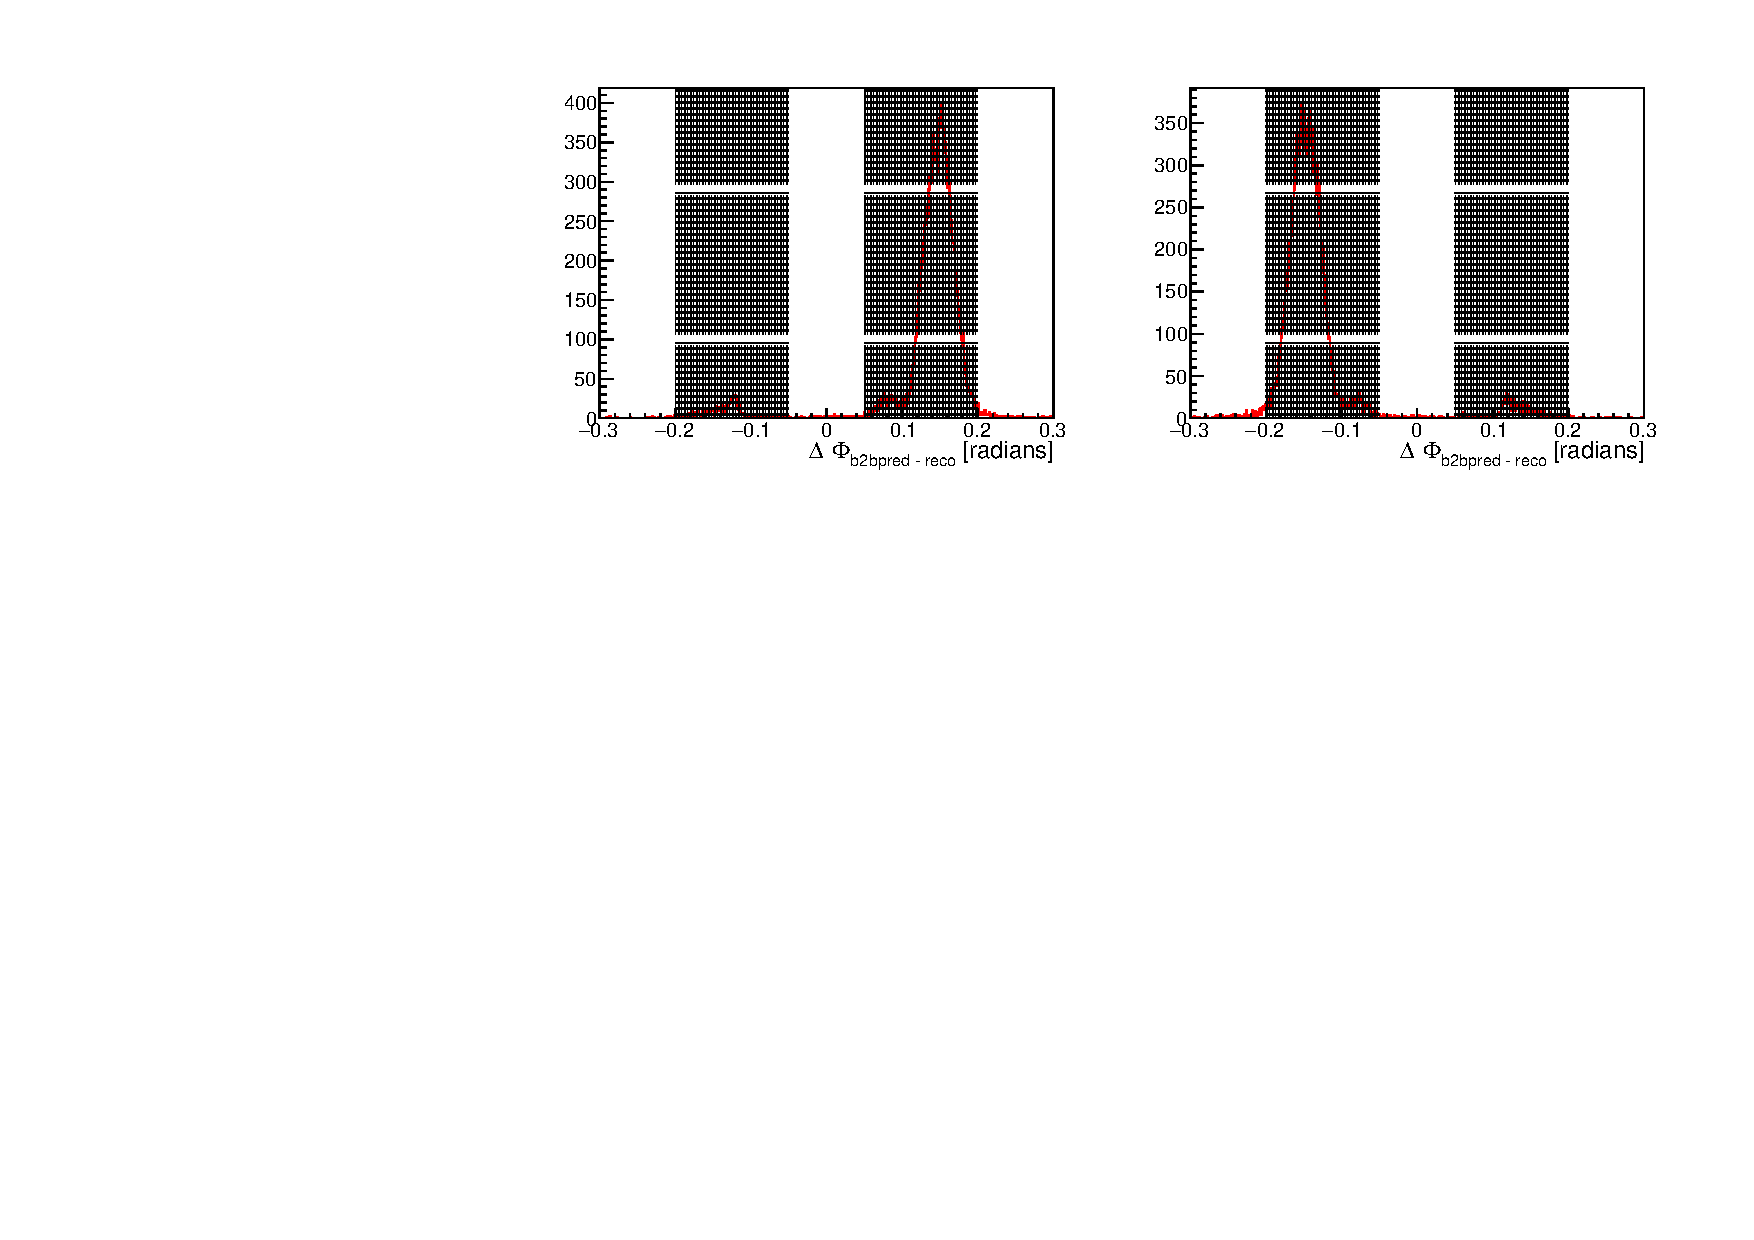
\includegraphics[width=\textwidth]{Plots/master/sb2b_MC.pdf}
	\caption[b2bClusterPhi - clusterPhi For MC]{Left: Predicted clusterPhi(HclE) - Reconstructed clusterPhi(LclE). Right: Predicted clusterPhi(LclE) - Reconstructed clusterPhi(HclE). Only particles within the gray area are taken into account. Both plots are created with phase2 MC. There is no middle peak because only $\textrm{ee} \rightarrow \textrm{ee}$ events were generated.}
	\label{fig:b2bMC}
\end{figure}







Figure \ref{fig:b2bMC} shows the same plots as figure \ref{fig:b2bData} but with phase2 MC. Note that there is no middle peak because only $\textrm{ee} \rightarrow \textrm{ee}$ events were generated. In figure \ref{fig:b2bMC_Whole} the b2bClusterPhi plot with full range is shown for MC.

\section{ECL-Trigger}
\label{sec:ECLTrigger}

Last but not least, we need to be sure that each event has a trigger signal coming from the ECL. Otherwise, the trigger signal could come only from the tracking detectors. Then, there would be a bias on the efficiency, since the tracking detectors require at least one track. Therefore, a cut on the trigger called \texttt{bhabha} is introduced. This trigger requires a signal coming from the ECL and some additional conditions. Both reconstructed particles have to have an energy of at least $2.5\,\textrm{GeV}$ each and one of them has to have at an energy of $4\,\textrm{GeV}$ or more. Also, two additional conditions have to be fulfilled. 

\begin{itemize} 
\item $160^\circ < \sum \theta_{cms} < 200^\circ$
\item $140^\circ < \Delta \phi_{cms} < 220^\circ$
\end{itemize}

The \texttt{bhabha} trigger returns a 1, only if all three conditions are fulfilled.
 \cite{lumeTrigger}

\begin{figure}[h!]
	\centering
	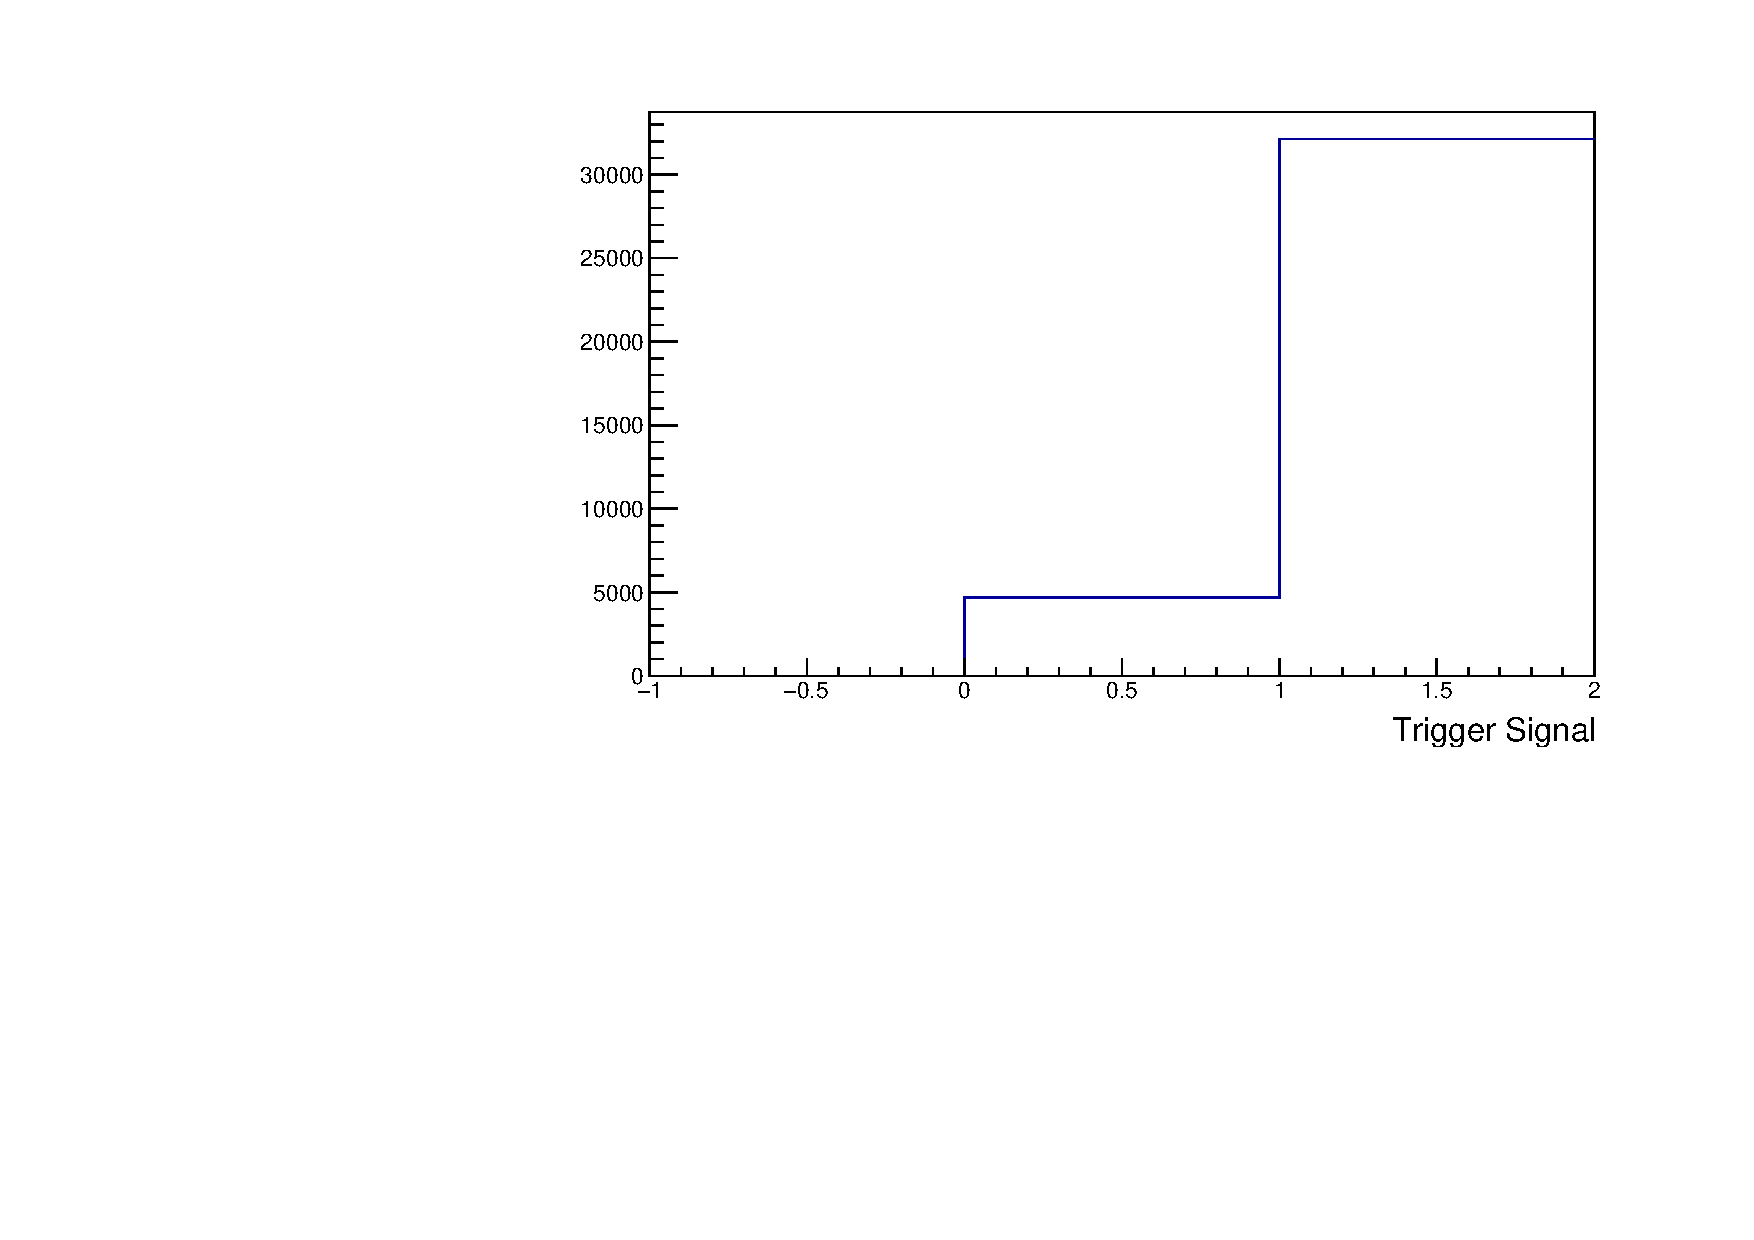
\includegraphics[width=\textwidth]{Cuts/Data/DataTrigger}
	\caption[\texttt{bhabha} Trigger Signal After Selection]{\texttt{bhabha} trigger signal for a single phase2 data file after the selection. 
		
		Trigger Signal == 0 means that there was no trigger signal in the event. Trigger Signal == 1 means that there was a trigger signal in the event. (Trigger Signal == -1 means that there are no trigger informations in the file.) As you can see, in most of the selected events there is a trigger signal coming from the ECL.}
	\label{fig:BhabhaTrigger}
\end{figure}

In figure \ref{fig:BhabhaTrigger} you can see the \texttt{bhabha} trigger signal for a single phase2 data file after the selection. Most of the time, there was an ECL trigger signal and in only about $8\,\%$ of the events there was no trigger signal coming from the ECL. These events have to be cut out.

This is not done for phase2 Monte Carlo, since the trigger does not work reliable on MC and we only look at events we want to consider. Therefore, a trigger cut is only done for phase2 data (and phase3 data in chapter \ref{chp:TrackingEfficiencyPhase3}). This is also the reason why the cuts on the cluster energy were chosen as they are. Otherwise, a comparison between phase2 MC and phase2 data would be impossible.

\section{More Events}
\label{sec:Phase2MoreEvents}





The efficiency errors are calculated with the following equation:

\begin{equation}
\Delta \epsilon = \sqrt{\frac{\epsilon(1-\epsilon)}{n}}
\label{eq:EffError}
\end{equation}

In equation \ref{eq:EffError}, $\epsilon$ is the calculated efficiency and $n$ is the total number reconstructed particles with and without an associated track in the investigated bin. This equation is only true for large $n$, since according this equation, an efficiency of 1 has always an error of zero. Therefore, the efficiency will be calculated by the root class TEfficiency. This class is able to calculate the right efficiency error even for small $n$. \cite{TEfficiency}



To reduce the error on the calculated efficiency, $n$ has to be as big as possible. Therefore, more phase2 data and phase2 MC files are needed. For Monte Carlo we will consider all files located at KEKCC: 
\newline

/belle/MC/release-01-00-02/DB00000294/MC10/prod00004668/s00/e1002/4S/
r00000/3600520000/mdst/sub00
\newline

Also, we will take all available phase2 data files into account. They are located on KEKCC at:
\newline

/ghi/fs01/belle2/bdata//Data/release-03-00-03/DB00000528/proc00000008/e0003/ 4S/r0*/all/mdst/sub00/*.root
\newline




\begin{figure}[h!]
	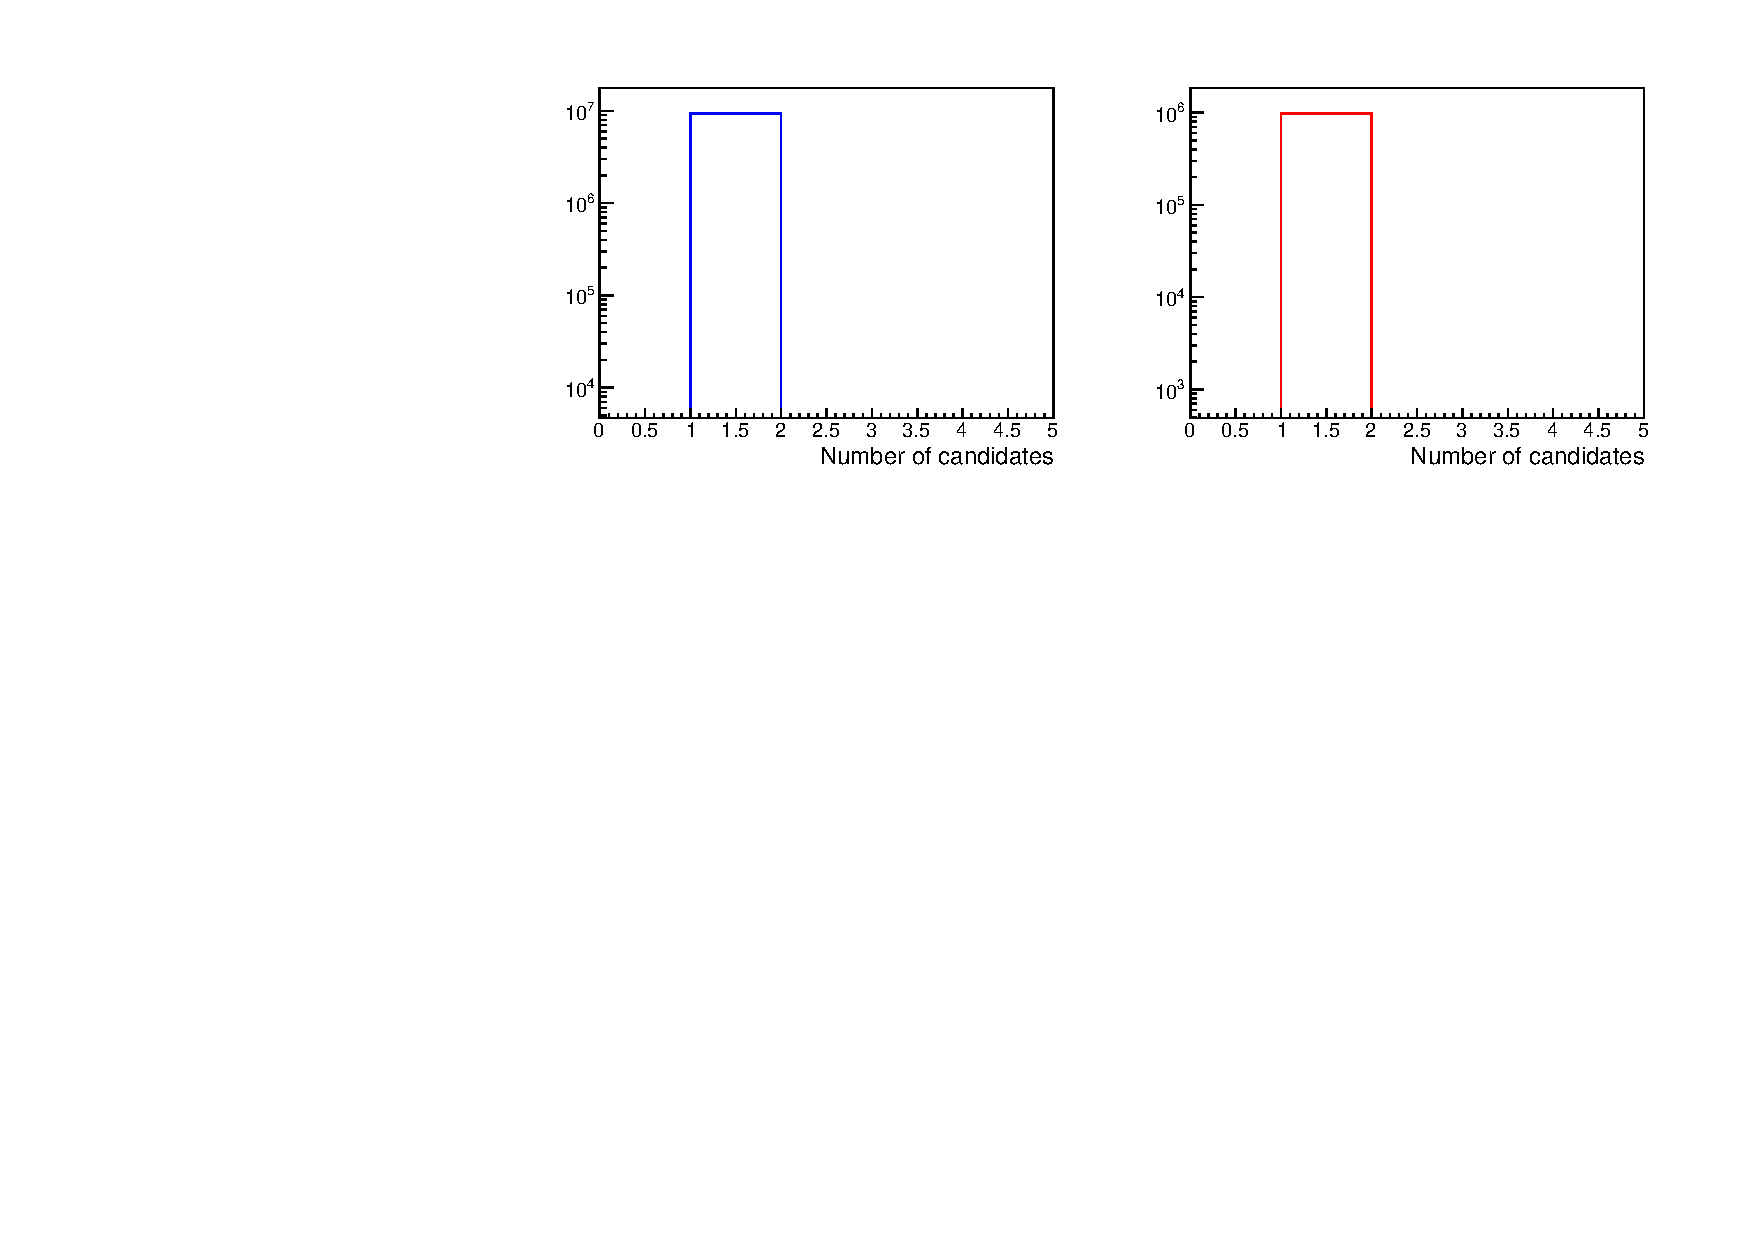
\includegraphics[width=\textwidth]{Plots/master/CCand.pdf}
	\caption[Total Number Of Events After The Selection]{The number of candidates per event after the selection is shown. Left: Phase2 Data. Right: Phase2 MC. A total of 9323903 candidates are selected for phase2 data and 973181 candidates are selected for phase2 MC.}
	\label{fig:nCandAS}
\end{figure}






In figure \ref{fig:nCandAS}, you can see the number of candidates per event after the selection. You can see that we reconstruct only one virtual photon per event on both phase2 data and phase2 MC.






\section{Dividing The ECL In Areas Of Interest}
\label{sec:DivECL}

As described in section \ref{sec:ECL}, the ECL is divided in three areas. The barrel, the forward end-cap and the backward end-cap. Therefore, we will take a look at the efficiency of these areas separately. The first area will only contain the forward end-cap. This means, only particles with an predicted $\theta$ angle of $0^\circ <\theta<32^\circ$ will be taken into account. The second area of interest is the barrel. Here the predicted $\theta$ angle of the investigated particle has to be $32^\circ < \theta < 130^\circ$. The last area of interest is the backward end-cap with an cluster $\theta$ angle of $130^\circ <\theta < 180^\circ$.  

In section \ref{sec:Kinematics}, we saw that the the azimuth angle and the momentum of the particles are correlated in the lab frame. Therefore, we need to look at momentum intervals. Otherwise, it would be impossible to interpret the calculated efficiencies. For example, a low efficiency in $\phi$ could be the results of an inefficient forward end-cap or created by momentum dependencies.




\begin{figure}[h!]
	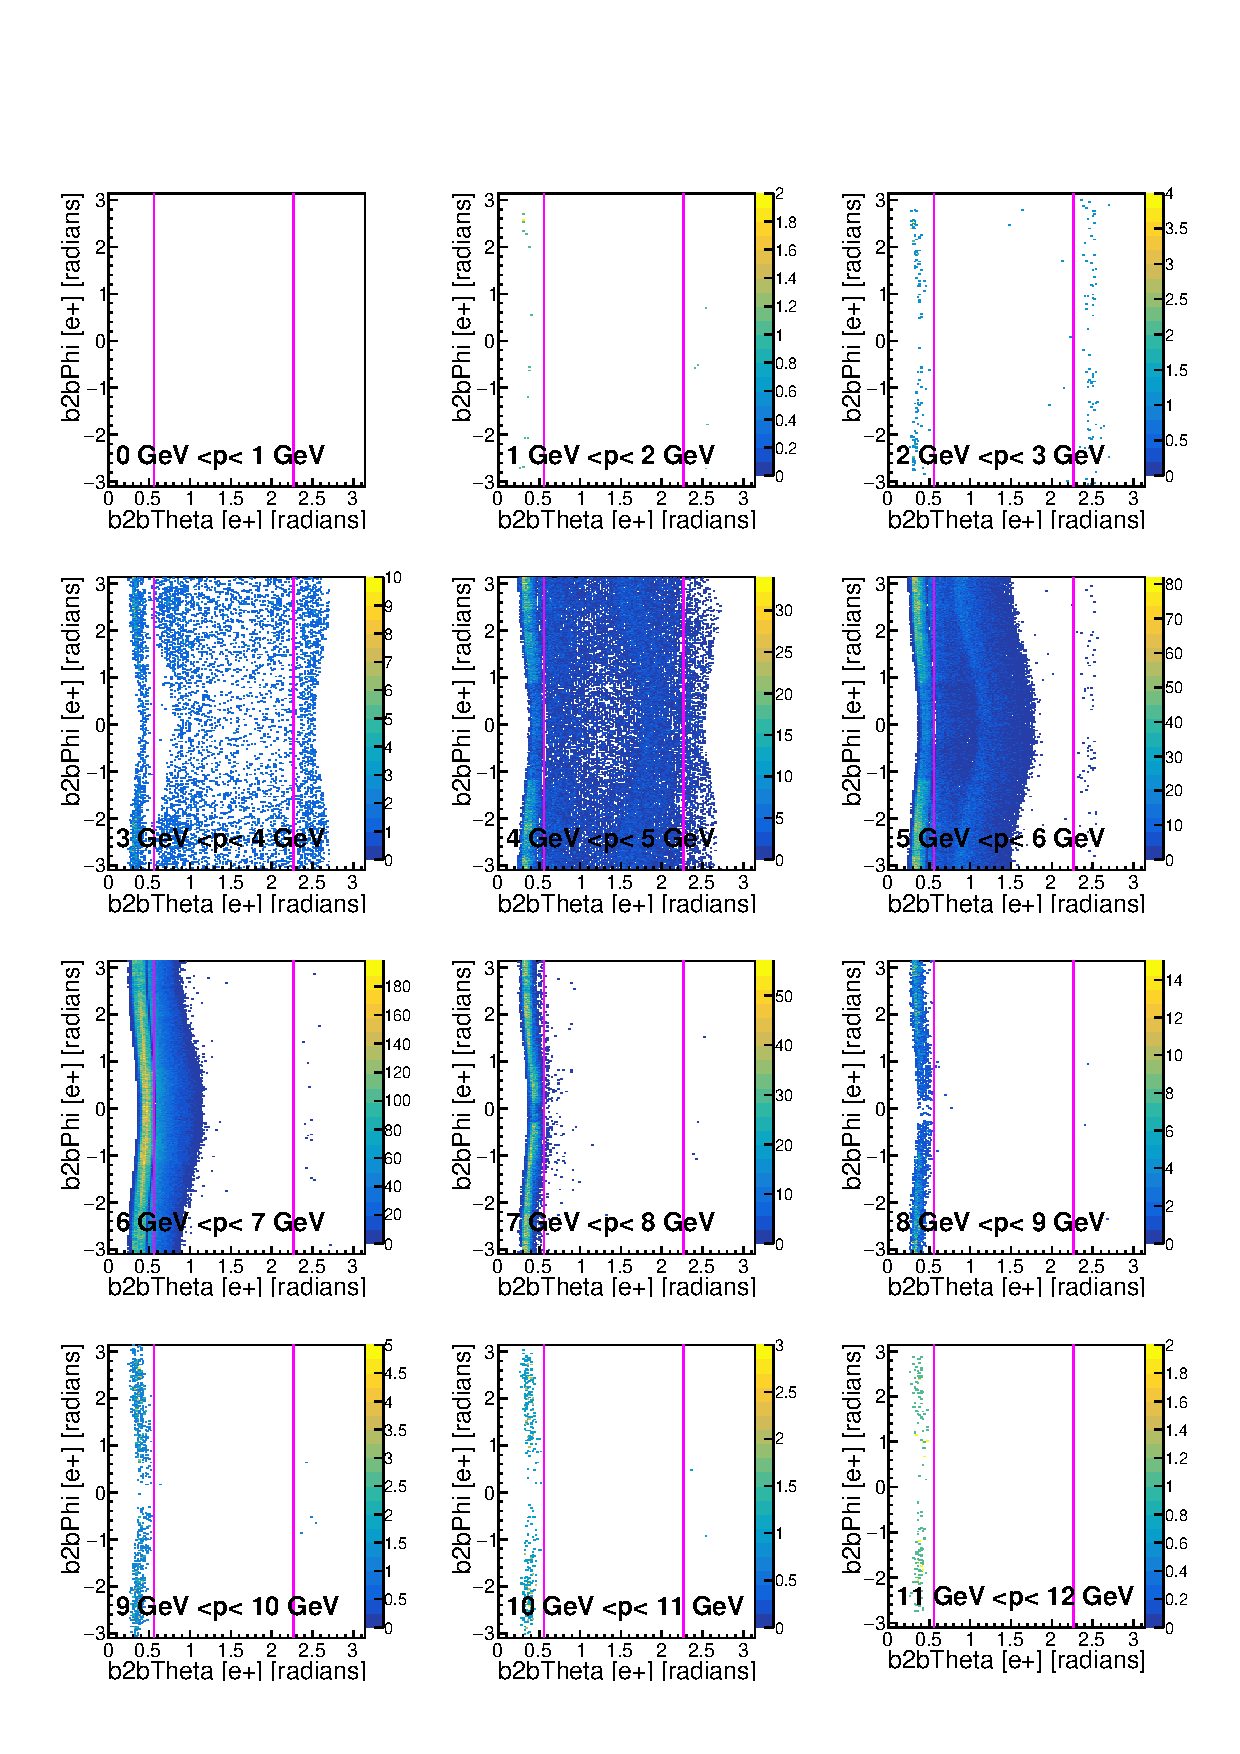
\includegraphics[width=\textwidth]{Plots/master/RTPMemD_MC.pdf}
	\caption[Denominator $\theta$-$\phi$ Electron Momentum MC]{Predicted $\theta$ and $\phi$ denominator histograms of the electron for different momenta for phase2 MC are shown. The different areas of interest are indicated by the pink line.}
	\label{plt:RTPMemD_MC}
\end{figure}

In figure \ref{plt:RTPMemD_MC} you can see the \textit{denominator} histograms for the electron. In these plots, the predicted $\theta$ and $\phi$ angles for different momenta for phase2 MC are shown. Also, the three areas of interest are indicated in these plots by a pink line. Phase2 MC was used to determine the momenta ranges because the statistics are lower on phase2 MC compared to phase2 data. 

\begin{figure}[h!]
	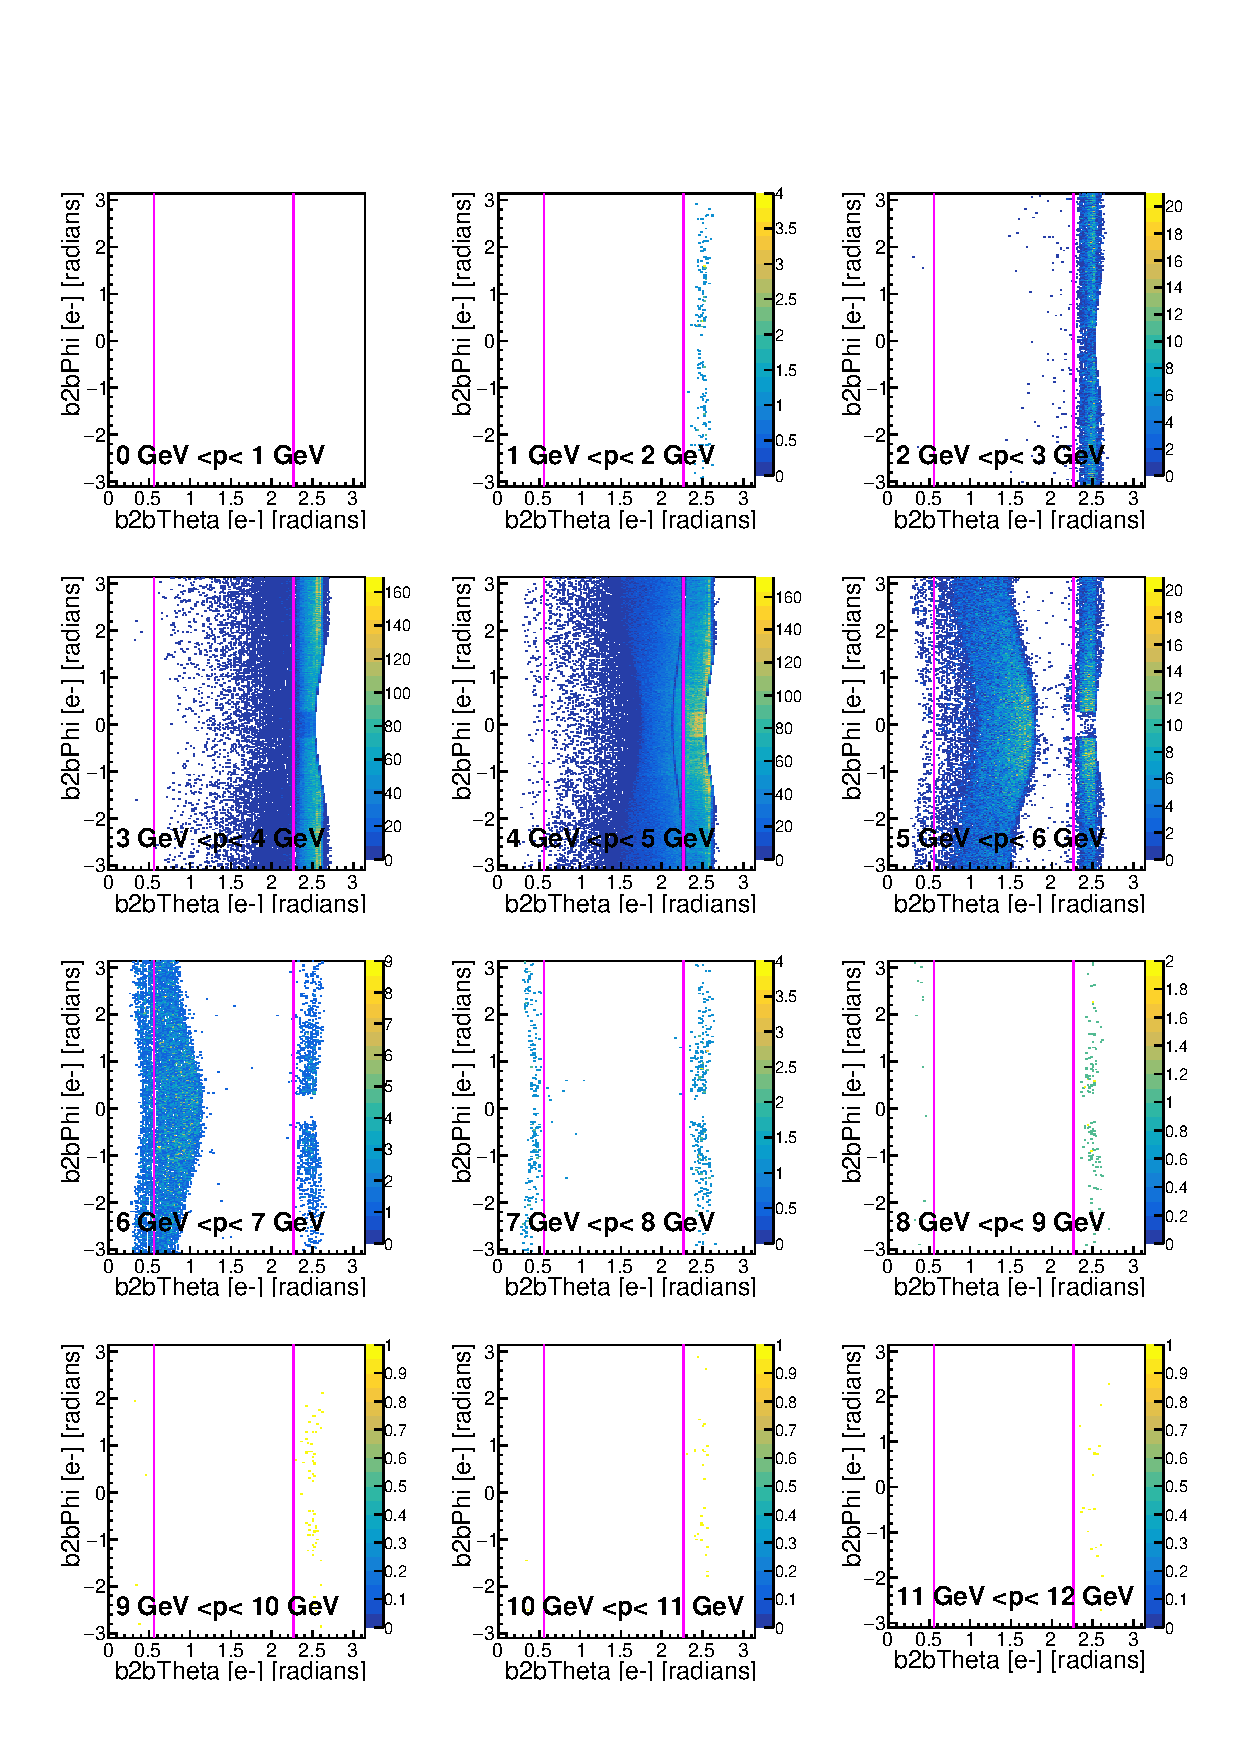
\includegraphics[width=\textwidth]{Plots/master/RTPMepD_MC.pdf}
	\caption[Denominator $\theta$-$\phi$ Positron Momentum MC]{Predicted $\theta$ and $\phi$ denominator histograms of the positron for different momenta phase2 MC are shown. The different areas of interest are indicated by the pink line.
	
}
	\label{plt:RTPMepD_MC}
\end{figure}


 Figure \ref{plt:RTPMemD_Data} shows the same plots but for phase2 data. Small differences for momenta between $4\,\textrm{GeV}$ and more at an $\phi$ angle of about $0^\circ$ are caused by the geometry of the vertex detector. As already mentioned in section \ref{sec:Phase2}, only a small azimuthal fraction at $\phi =0$ was installed but not simulated properly on Monte Carlo. 
 The corresponding phase2 data plots for positrons are shown in figure \ref{plt:RTPMepD_Data}.  

In these four figures, one can also see that it makes sense to look only at some momenta for different areas of interest. The different momenta regions are listed in table \ref{tab:RTPMDTable}.


\begin{table}[h!]
	\centering
	\begin{tabular}{lccc}
		&$\textrm{e}^-$ &$\textrm{e}^+$\\
		\hline
		Forward End-Cap &$4\,\textrm{GeV} - 8\,\textrm{GeV}$&/\\
		Barrel &$4\,\textrm{GeV} - 7\,\textrm{GeV}$&$3\,\textrm{GeV} - 7\,\textrm{GeV}$\\
		Backward End-Cap & /&$2\,\textrm{GeV} - 6\,\textrm{GeV}$\\	
	\end{tabular}
	
	\caption[Areas Of Interest Different Momenta Ranges]{Momenta ranges for different \textit{probe} cases and different areas of interest.}
	\label{tab:RTPMDTable}
\end{table}





\begin{figure}[h!]
	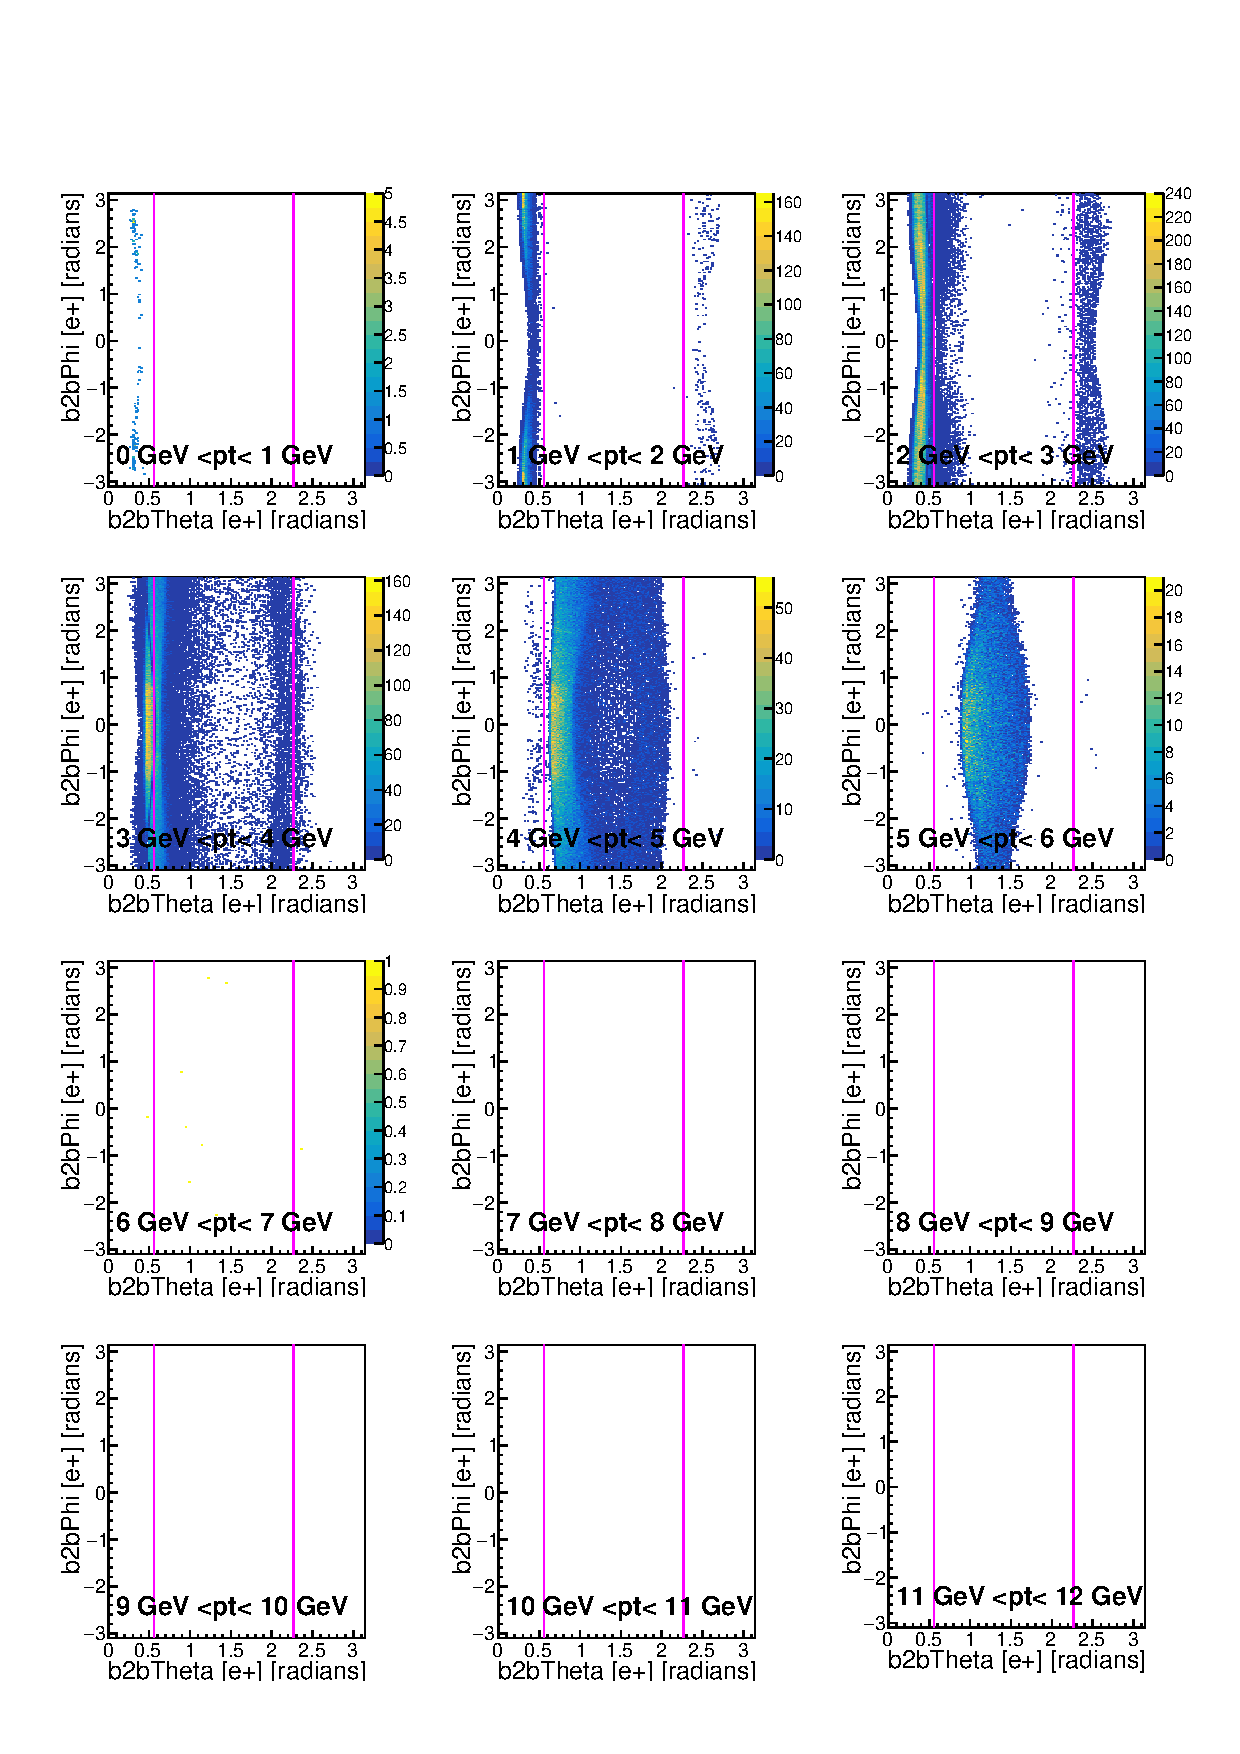
\includegraphics[width=\textwidth]{Plots/master/RTPtMemD_MC.pdf}
	\caption[Denominator $\theta$-$\phi$ Electron Transverse Momentum MC]{Predicted $\theta$ and $\phi$ denominator histograms of the electron for different transverse momenta for phase2 MC are shown. The different areas of interest are indicated by the pink line.
}
	\label{plt:RTPtMemD_MC}
\end{figure}



\begin{figure}[h!]
	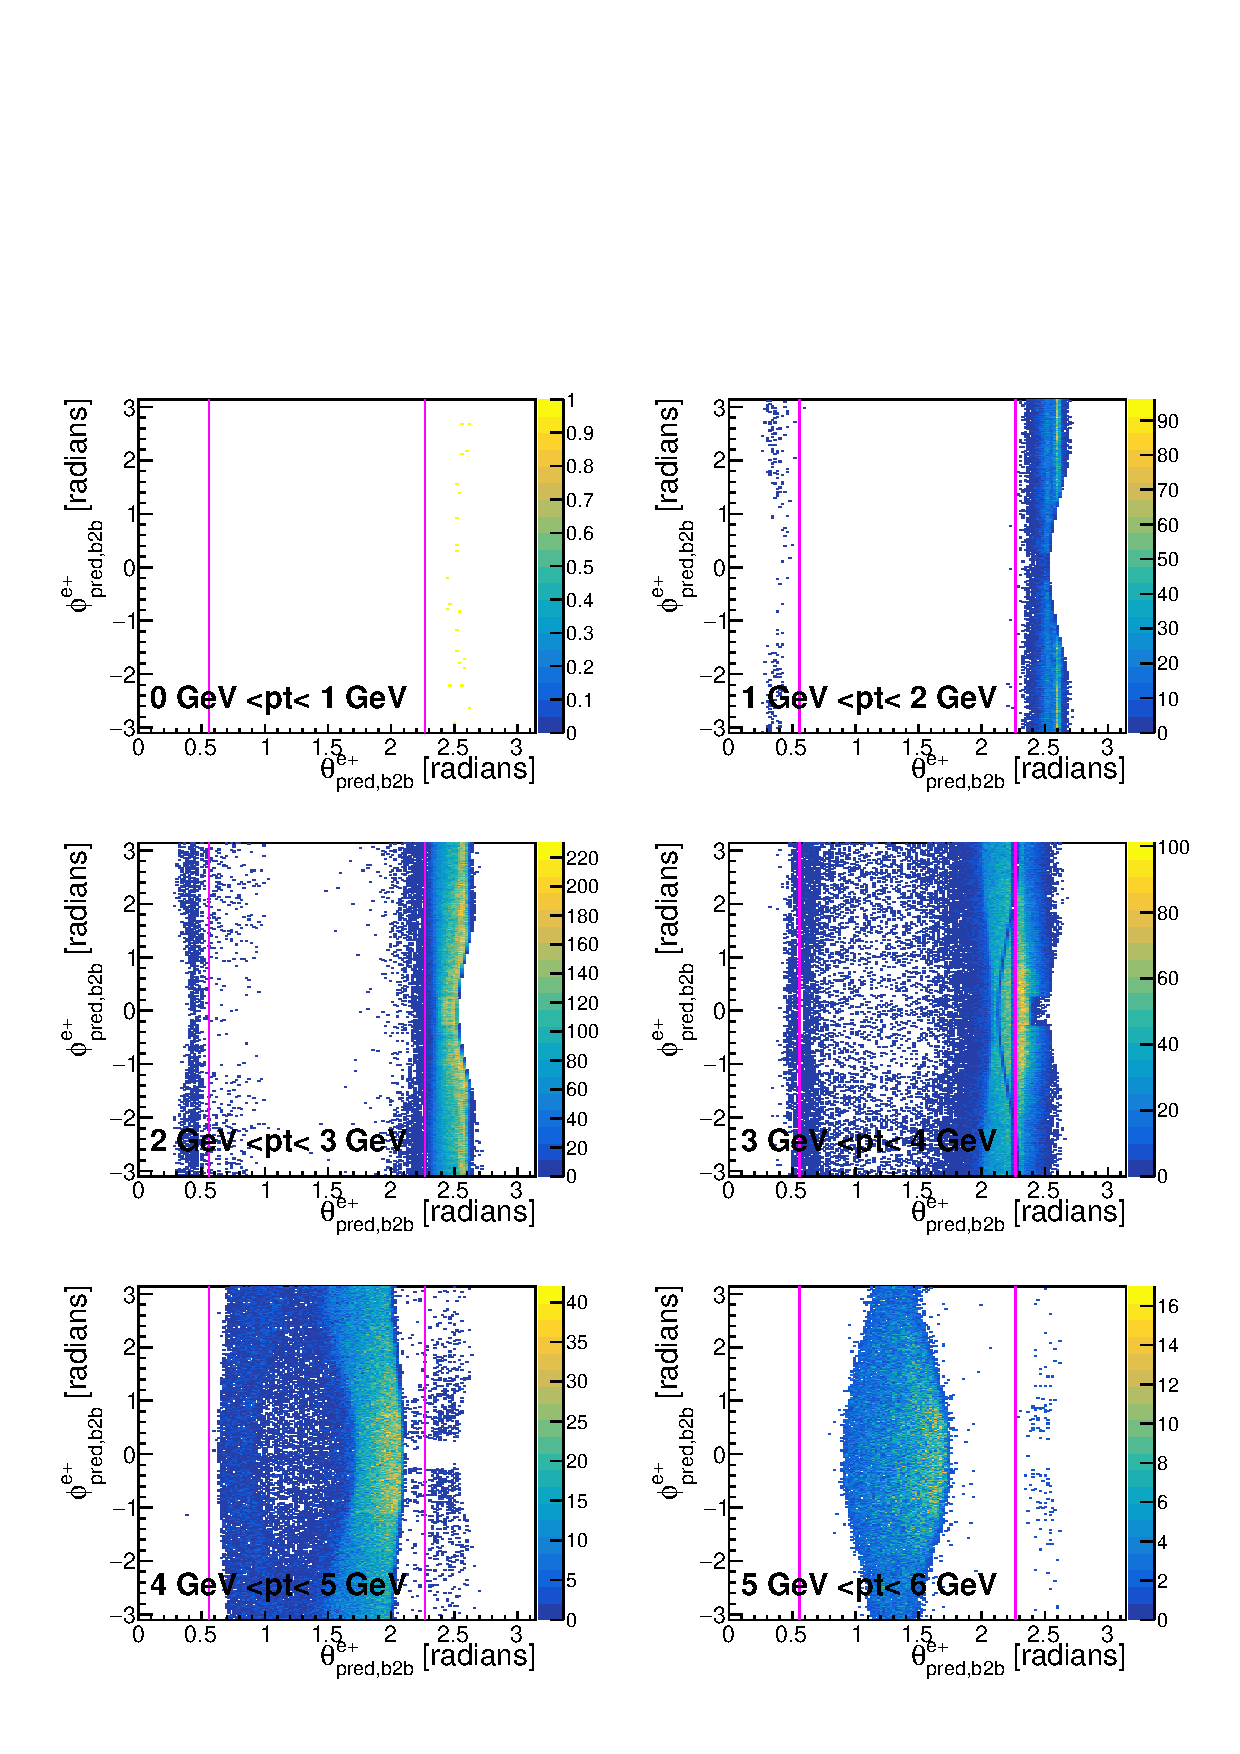
\includegraphics[width=\textwidth]{Plots/master/RTPtMepD_MC.pdf}
	\caption[Denominator $\theta$-$\phi$ Positron Transverse Momentum MC]{Predicted $\theta$ and $\phi$ denominator histograms of the positron for different transverse momenta for phase2 MC are shown. The different areas of interest are indicated by the pink line.
}
	\label{plt:RTPtMepD_MC}
\end{figure}


The same is done for the transverse momenta for the three different cases. The denominator plots of phase2 MC for the electrons can be seen in figure \ref{plt:RTPtMemD_MC}. Figure \ref{plt:RTPtMepD_MC} shows the denominator plots for phase2 MC positrons. The different transverse momenta regions are listed in table \ref{tab:RTPtMDTable}.







\begin{table}[h!]
	\centering
	\begin{tabular}{lccc}
		&$\textrm{e}^-$ &$\textrm{e}^+$\\
		\hline
		Forward End-Cap &$1\,\textrm{GeV} - 4\,\textrm{GeV}$&/\\
		Barrel &$2\,\textrm{GeV} - 6\,\textrm{GeV}$&$3\,\textrm{GeV} - 6\,\textrm{GeV}$\\
		Backward End-Cap & /&$1\,\textrm{GeV} - 4\,\textrm{GeV}$\\
	\end{tabular}
	
	\caption[Areas Of Interest Different Transverse Momenta Ranges]{Transverse Momenta ranges for different \textit{probe} cases and different areas of interest.}
	\label{tab:RTPtMDTable}
\end{table}








We will also look at the tracking efficiency as a function of $\theta$. For this, we also have to choose momenta regions. They can be determined by the same plots as before.
The selected ranges can be found in table \ref{tab:RTPMDThetaTable}.

\begin{table}[h!]
	\centering
	\begin{tabular}{lccc}
		&$\textrm{e}^-$ &$\textrm{e}^+$\\
		\hline
		Momentum &$4\,\textrm{GeV} - 9\,\textrm{GeV}$&$2\,\textrm{GeV} - 7\,\textrm{GeV}$\\
		Transverse Momentum &$1\,\textrm{GeV} - 6\,\textrm{GeV}$&$1\,\textrm{GeV} - 6\,\textrm{GeV}$\\

	\end{tabular}
	
	\caption[Different (Transverse-) Momenta Ranges For $\theta$ Efficiency]{Momenta and transverse momenta ranges for the tracking efficiency as a function of $\theta$.}
	\label{tab:RTPMDThetaTable}
\end{table}




\chapter{Phase2 Tracking Efficiency}
\label{chp:TrackingEfficiencyPhase2}



\lettrine{I}{n} this chapter the tracking efficiency studies on phase2 will be presented. The selection described in chapter \ref{chap:Phase2Eff} will be applied in this chapter. Phase2 data in blue and phase2 Monte Carlo in red will be shown together, in order to make comparison between these two easier. The individual tracking efficiencies can be found in the appendix chapter \ref{A:2}. Also, only tracking efficiencies with $\Delta \epsilon < 0.4$ are plotted to make the plots more easy to read. 
 

\section{Momentum Efficiencies}


\subsection{Forward End-Cap}
\label{sec:MFC}


In figure \ref{plt:xPMPhiemFC} you can see the calculated electron tracking efficiency for different momenta. As expected, the tracking efficiency for phase2 data is almost all of the time worse than the efficiency for phase2 MC for all momenta. For momenta between $4\,\textrm{GeV}$ and $5\,\textrm{GeV}$, phase2 MC and phase2 data have a similar efficiency. In both cases, the lowest efficiency occurs at $\phi \approx 0$. According to figures \ref{plt:RTPMemD_MC} and \ref{plt:RTPMemD_Data}, we expect that most electrons have a momentum between $5\,\textrm{GeV}$ and $8\,\textrm{GeV}$. For momenta between $5\,\textrm{GeV}$ and $6\,\textrm{GeV}$ phase2 data and phase2 MC have some differences in the calculated tracking efficiency. Phase2 MC has an efficiency between 0.80 and 0.95 with an exception of an efficiency drop at $\phi \approx 0$. This drop also appears on phase2 data, but for $\phi > \textrm{abs}(1.5)$ the efficiency on phase2 data is much worse than phase2 MC. Here the efficiency falls partially below 0.7 for phase2 data.
 The biggest difference occurs for momenta between $6\,\textrm{GeV}$ and $7\,\textrm{GeV}$. For phase2 MC, the tracking efficiency ranges between 0.90 and almost 1.00. But the efficiency oscillates heavily between 0.7 and 0.95 for phase2 data. In both cases the highest efficiency occurs at $\phi \approx 0$. For momenta between $7\,\textrm{GeV}$ and $8\,\textrm{GeV}$, phase2 MC has a tracking efficiency of above 0.98 for all $\phi$ angles. Except for $\phi \approx 0$. Here the efficiency is still high but the errors are bigger. For phase2 data, the efficiency is also very high for $\phi >\textrm{abs}(1)$. But for $\phi < \textrm{abs}(1)$ the efficiency falls down by over $10\,\%$.






\begin{figure}[!htbp]
	\centering
	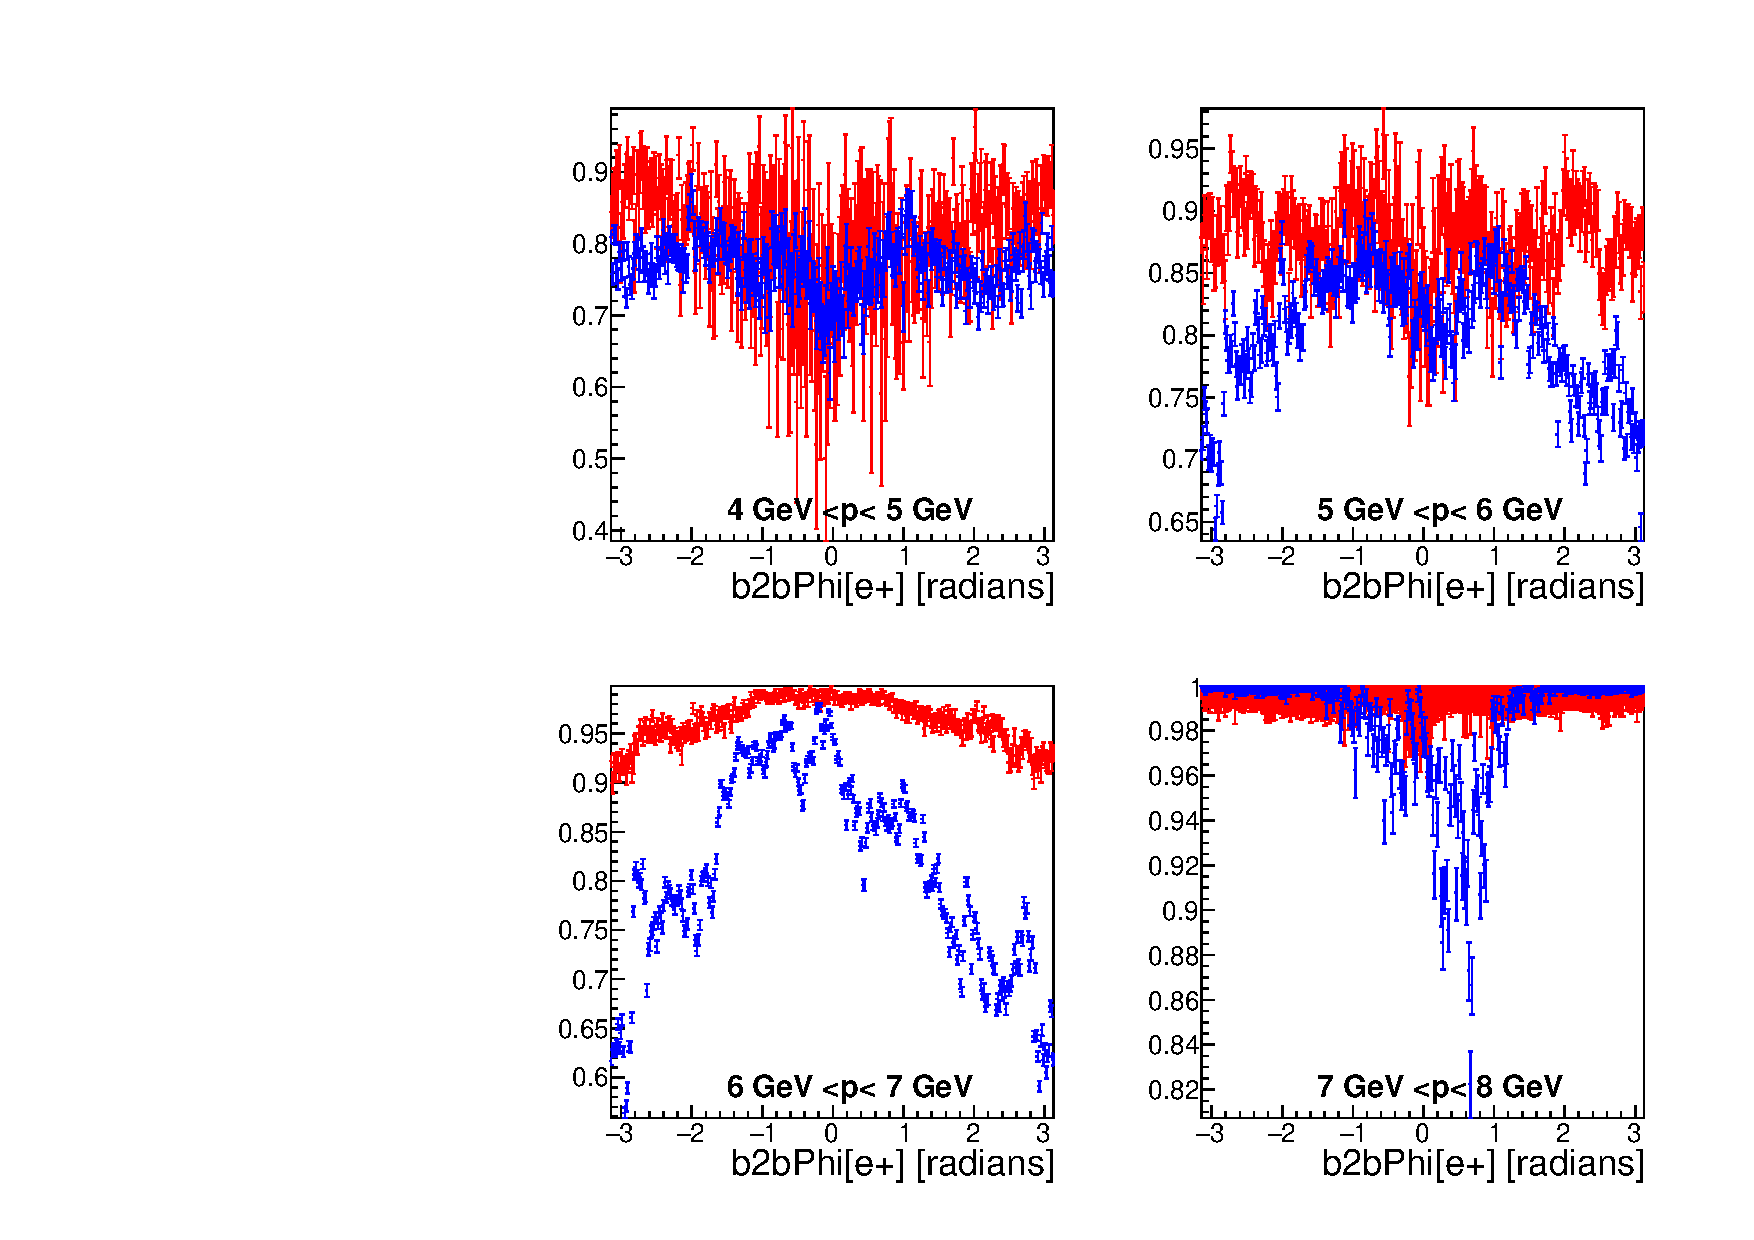
\includegraphics[width=\textwidth]{Plots/master/xPMPhiemFC}
	\caption[Momentum $\phi$ Electron Forward End-Cap Efficiency Phase2]{Electron $\phi$ tracking efficiency plots in the forward end-cap. The tracking efficiency for phase2 data is shown in blue and phase2 MC in red.}
		\label{plt:xPMPhiemFC}
\end{figure}







\newpage



\subsection{Barrel}

In figure \ref{plt:xPMPhiemBarrel} the calculated electron tracking efficiency in the barrel is shown. For momenta between $4\,\textrm{GeV}$ and $5\,\textrm{GeV}$ the tracking efficiency is between 0.75 and 0.96 for phase2 MC and between 0.77 and 0.93 for phase2 data. For phase2 data the efficiency has its minimum at $\phi \approx 0$. For momenta between $5\,\textrm{GeV}$ and $6\,\textrm{GeV}$, the efficiency gets better. The tracking efficiency ranges between 0.90 and 0.99 for phase2 MC and between 0.91 and 0.98 for phase2 data. The structure of this efficiency is very similar compared to the tracking efficiency for momenta between $4\,\textrm{GeV}$ and $5\,\textrm{GeV}$. In both cases the lowest efficiency occurs at $\phi \approx 0$ for phase2 data. The best tracking efficiencies for electrons in the barrel appear at momenta between $6\,\textrm{GeV}$ and $7\,\textrm{GeV}$. Here the efficiency for phase2 MC is between 0.98 and 1 and for phase2 data between 0.955 and 0.995. Again, the lowest calculated tracking efficiency occurs at  $\phi \approx 0.5$. Without this drop, the tracking efficiency of phase2 data is between 0.980 and 0.995. 

The calculated tracking efficiencies for positrons in the barrel can be found in figure \ref{plt:xPMPhiepBarrel}. You can see that for momenta between $3\,\textrm{GeV}$ and $4\,\textrm{GeV}$, the calculated tracking efficiency is between 0.7 and 0.98 for phase2 MC and between 0.7 and 0.92 for phase2 data.The efficiency for phase2 MC stays more or less the same over all values of $\phi$. For phase2 data, there is an efficiency drop at $\phi \approx 0$.

For momenta between $4\,\textrm{GeV}$ and $5\,\textrm{GeV}$ the tracking efficiency is between 0.97 and 1 for phase2 MC and between 0.96 and 0.99 for phase2 data. Phase2 data has almost always a lower calculated tracking efficiency than phase2 MC.
The biggest difference between phase2 data and phase2 MC appears at $\phi \approx 0.5$. Here, the efficiency for phase2 data falls down significantly. 
For momenta between $5\,\textrm{GeV}$ and $6\,\textrm{GeV}$, the tracking efficiency ranges between 0.93 and 1 for phase2 MC and 0.95  and 0.99 for phase2 data. The tracking efficiency for phase2 MC is higher by 0.02 compared to phase2 data for almost all $\phi$ angles. 
For momenta between $6\,\textrm{GeV}$ and $7\,\textrm{GeV}$, the phase2 MC tracking efficiency ranges between 0.75 and 1. This wide range is a result of the low statistic for positrons at this momentum. The calculated tracking efficiency for phase2 data ranges between 0.9 and 1. For all tracking efficiencies with momenta between $4\,\textrm{GeV}$ and $7\,\textrm{GeV}$, you can see a dip at $\phi \approx 0.5$.



\begin{figure}[!htbp]
	\centering
	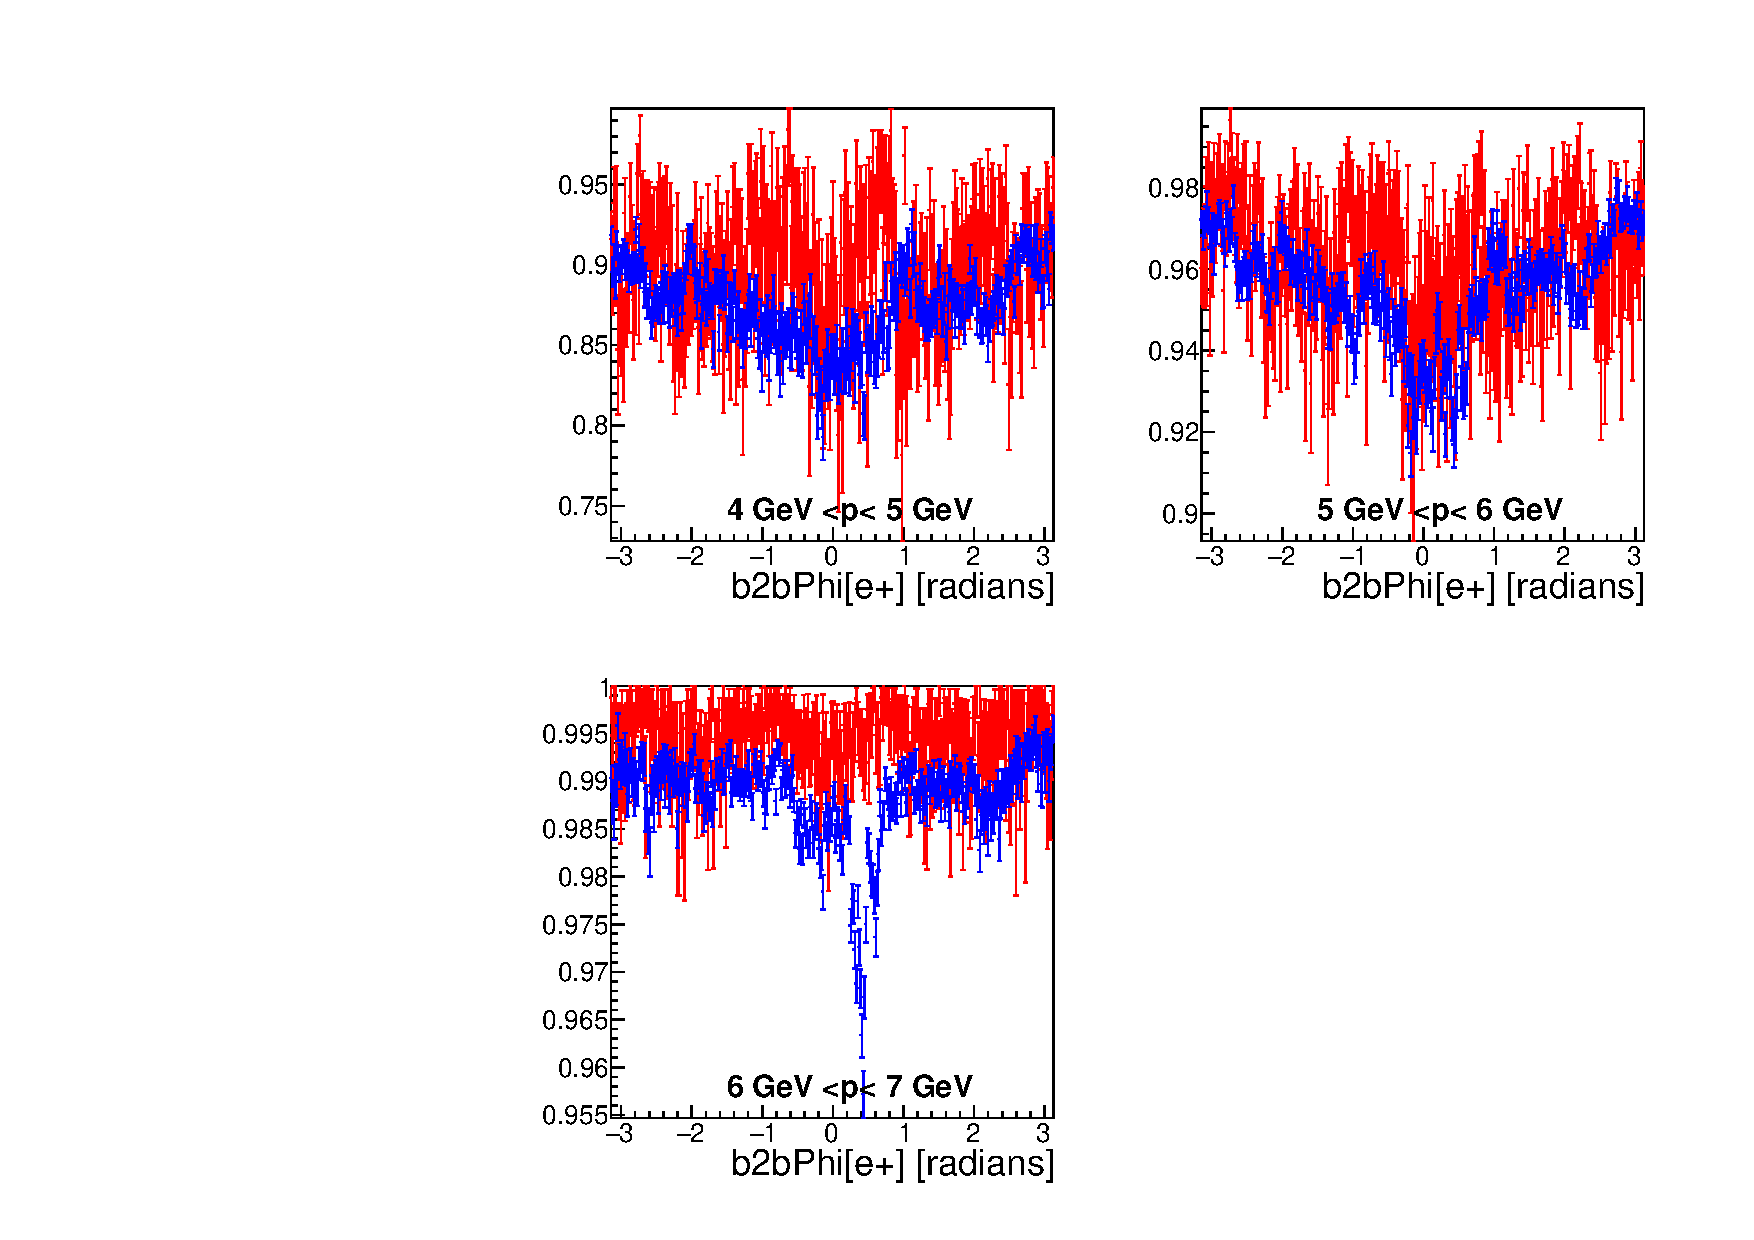
\includegraphics[width=\textwidth]{Plots/master/xPMPhiemBarrel}
	\caption[Momentum $\phi$ Electron Barrel Efficiency Phase2]{Electron $\phi$ tracking efficiency plots in the barrel. The tracking efficiency for phase2 data is shown in blue and phase2 MC in red.}
	\label{plt:xPMPhiemBarrel}
\end{figure}




\begin{figure}[!htbp]
	\centering
	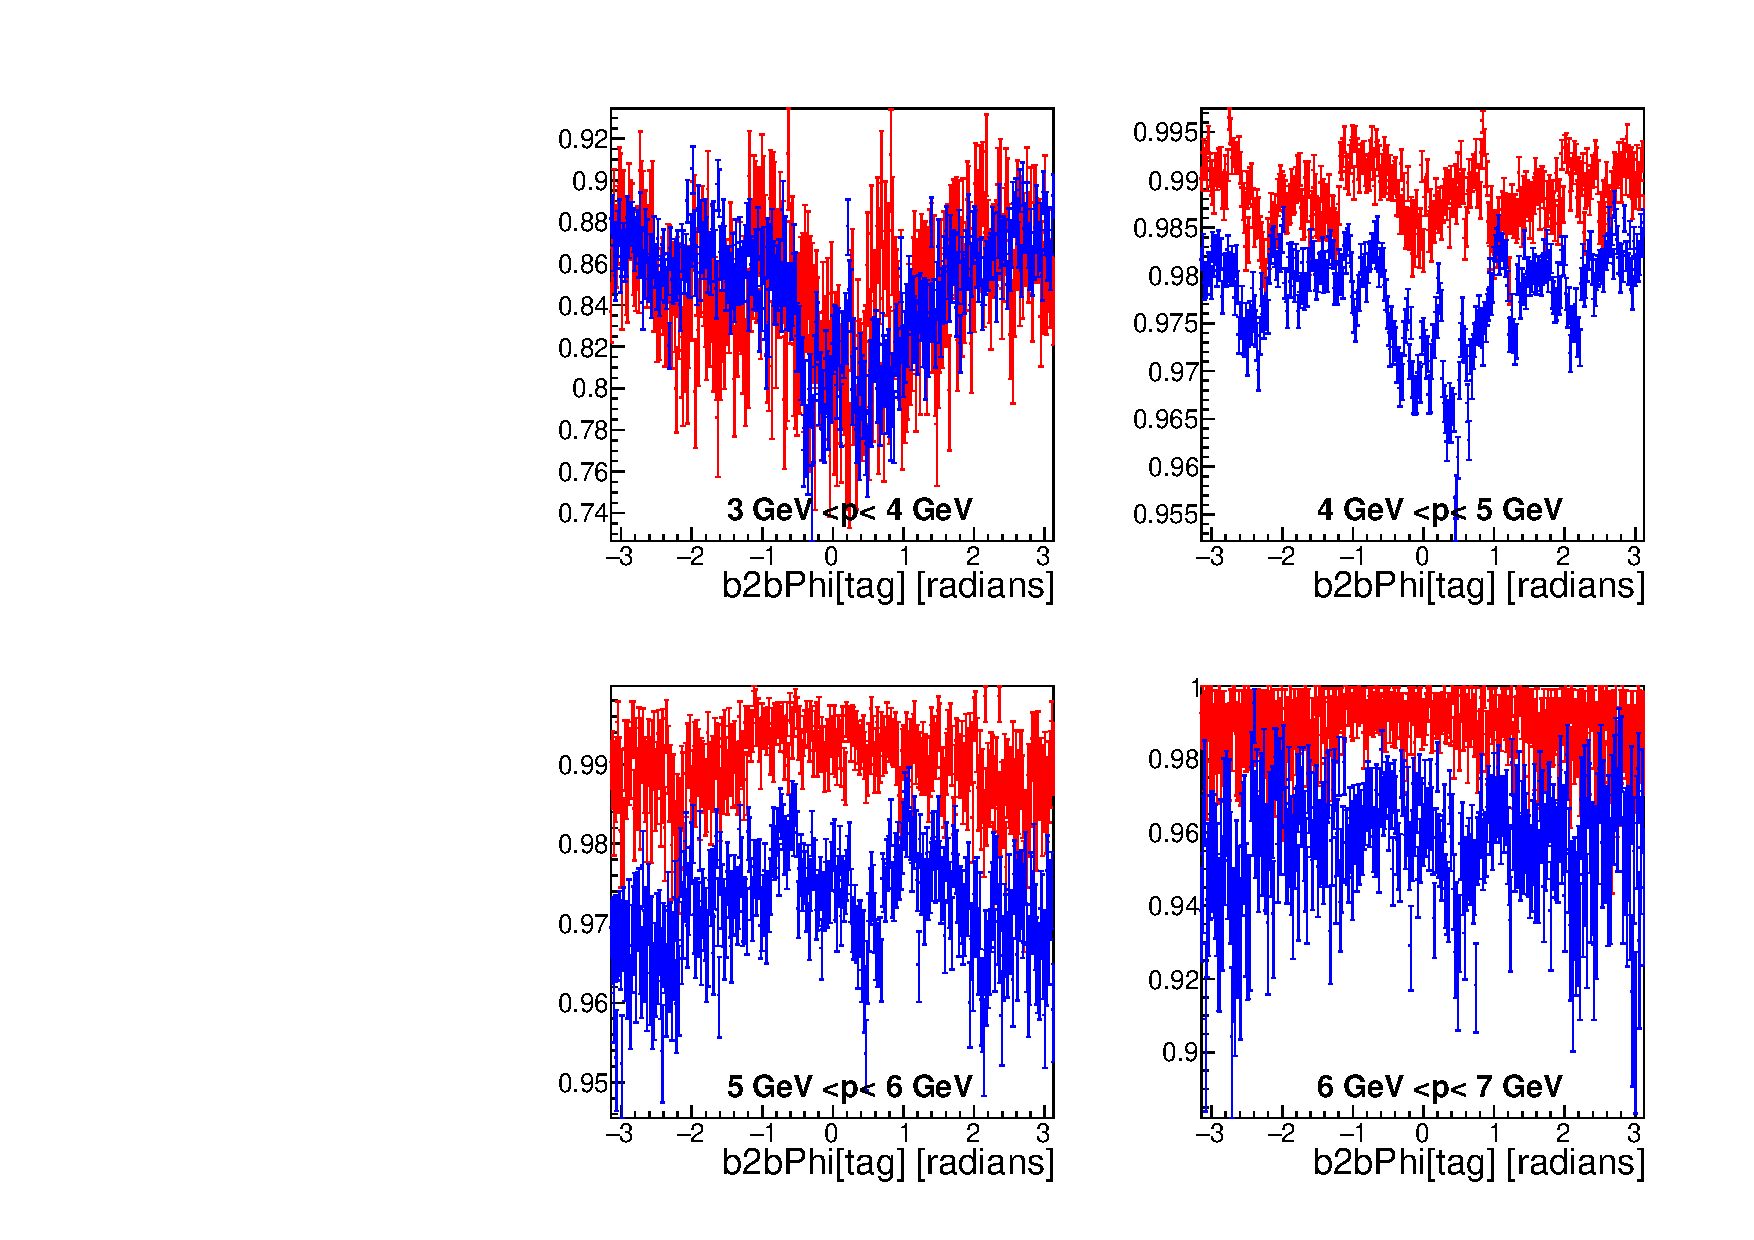
\includegraphics[width=\textwidth]{Plots/master/xPMPhiepBarrel}
	\caption[Momentum $\phi$ Positron Barrel Efficiency Phase2]{Positron $\phi$ tracking efficiency plots in the barrel. The tracking efficiency for phase2 data is shown in blue and phase2 MC in red.}
		\label{plt:xPMPhiepBarrel}
\end{figure}

\newpage
\subsection{Backward End-Cap}
\label{sec:MEC}

In figure \ref{plt:xPMPhiepEC} you can see the calculated positron tracking efficiency for different momenta in the backward end-cap. 
Due to the kinematics at Belle II, almost no electrons are detected in the backward end-cap. For momenta between $2\,\textrm{GeV}$ and $3\,\textrm{GeV}$, the calculated tracking efficiency is between 0.95 and 1 for phase2 data and between 0.85 and 1 for phase2 MC. An exception occurs at $\phi \approx 0$, here the error bars for phase2 MC are noticeably large. 
For momenta between $3\,\textrm{GeV}$ and $4\,\textrm{GeV}$ the tracking efficiency covers a very large range. For phase2 MC the efficiency is between 0.4 and 0.95 and for phase2 data between 0.2 and 0.85. For $\phi <  -1$, the efficiency is slightly higher for phase2 data compared to phase2 MC. 
A strange structure occurs at $\phi \approx 0$ for phase2 data. Starting at around $\phi \approx -1.7$ the efficiency goes up from 0.4 to 0.65 at $\phi \approx -0.8$, then it goes back down to 0.4 before it reaches a maximum of 0.8 at $\phi \lesssim 0$.
At $\phi =0$ the efficiency is down to $\sim 0.6$. At $\phi \gtrsim 0$, the efficiency is back to a maximum of 0.85 before it falls back down to $\sim 0.4$.
After that, the efficiency stays constant until it starts to fall down again at $\phi \approx 1.5$. It reaches its minimum at $\phi \approx 2$.
For phase2 MC the calculated tracking efficiency starts similar to phase2 data at around 0.5 and it slowly increases until $\phi \approx -1$. Than it starts to vary from phase2 data. For phase2 MC the efficiency  increases rapidly until it reaches its maximum at $\phi = 0$. Then it falls back to 0.6 at $\phi \approx 1$.
A similar structure can be found for momenta between $4\,\textrm{GeV}$ and $5\,\textrm{GeV}$. The only difference is that the efficiency is higher compared to the lower momenta. For example, phase2 MC reaches a calculated tracking efficiency of almost 1 at $\phi =0$.
For momenta between $5\,\textrm{GeV}$ and $6\,\textrm{GeV}$ the efficiency is above 0.9 for  phase2 MC and above 0.98 for phase2 data with the exception of $\phi \approx 0$. Here, the error of the calculated efficiencies are very large in both cases due to the low statistics.





\begin{figure}[!htbp]
	\centering
	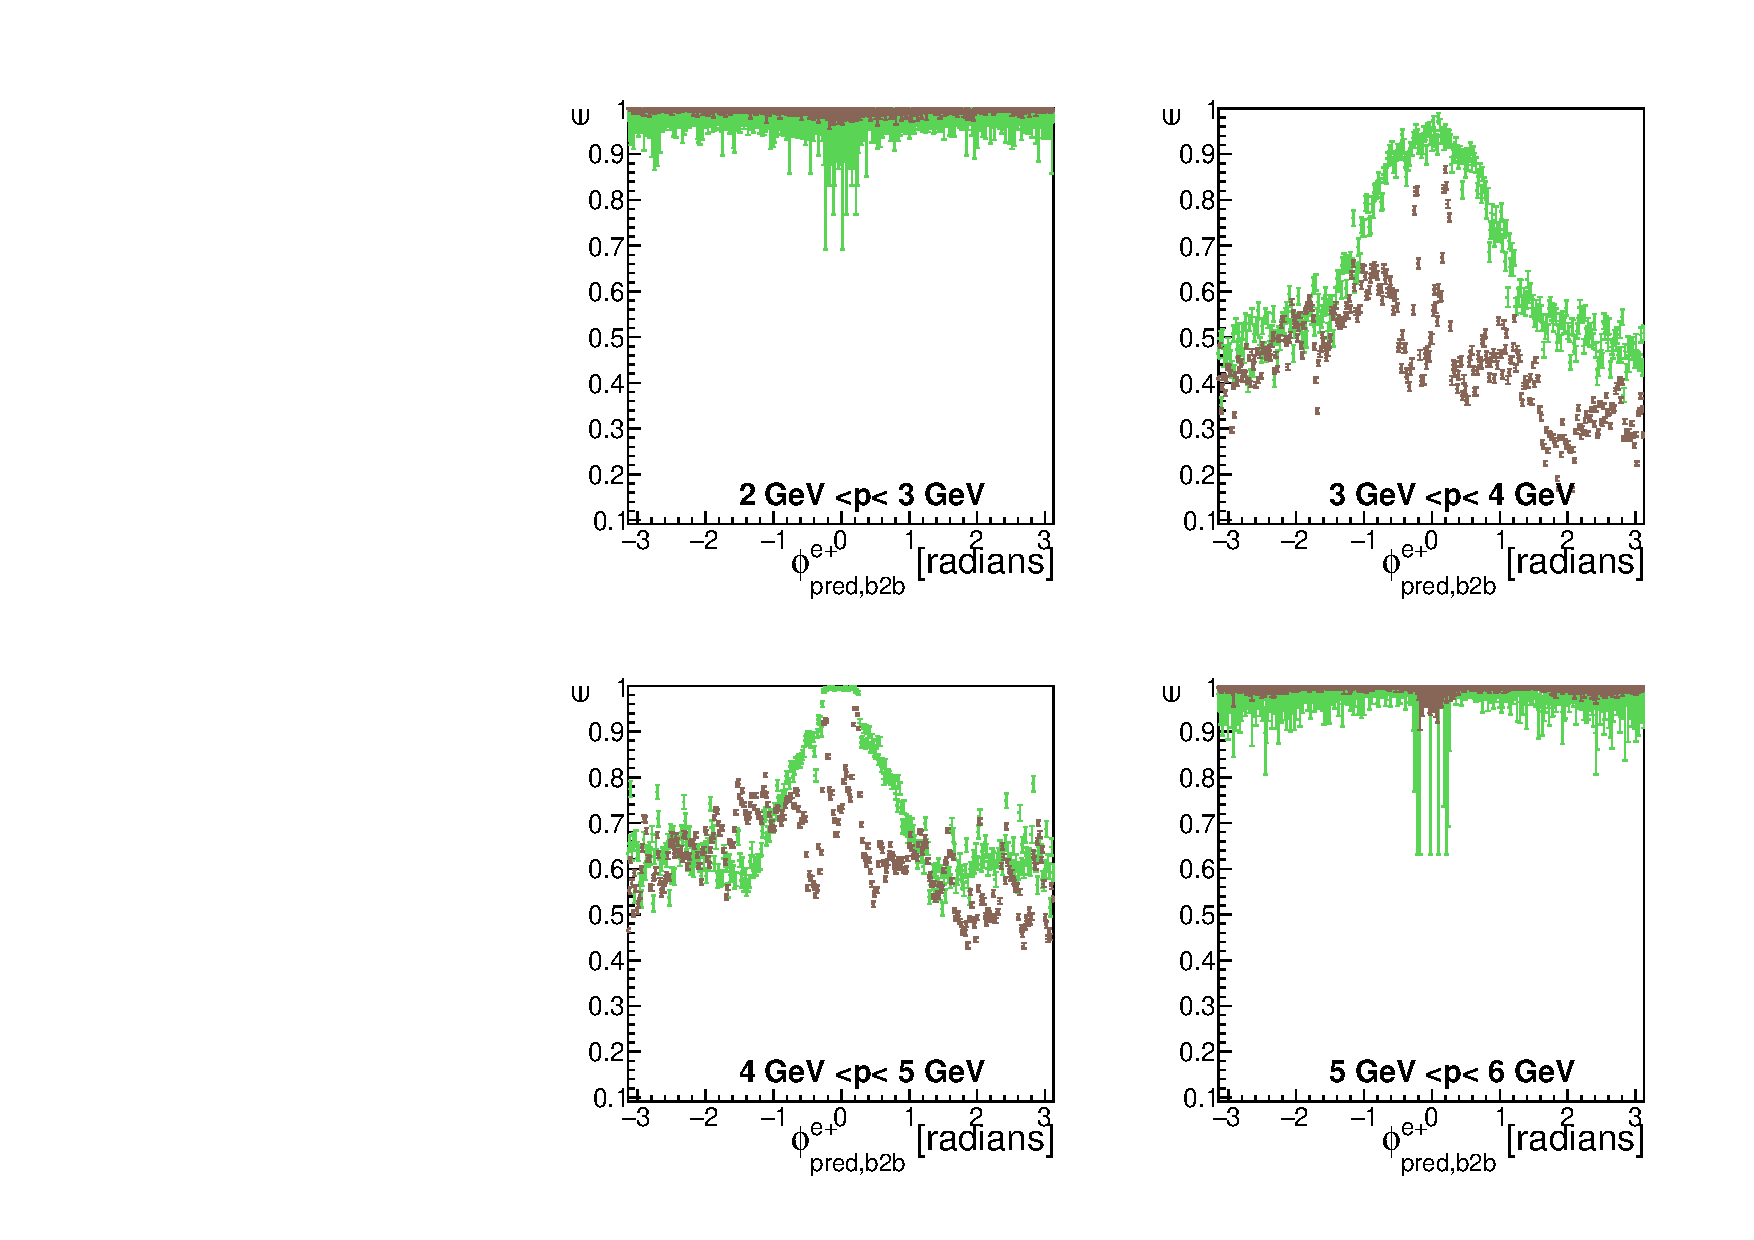
\includegraphics[width=\textwidth]{Plots/master/xPMPhiepEC}
	\caption[Momentum $\phi$ Positron Backward End-Cap Efficiency Phase2]{Positron $\phi$ tracking efficiency plots in the backward end-cap. The tracking efficiency for phase2 data is shown in blue and phase2 MC in red.}
	
	\label{plt:xPMPhiepEC}
\end{figure}









\clearpage




\subsection{$\theta$ Efficiencies}

This section will present the calculated tracking efficiencies as a function of the polar angle $\theta$. The pink lines in each of the following plots will indicate the different areas of the ECL.

Figure \ref{plt:xPMThetaem} shows the calculated electron tracking efficiency for different momenta as a function of the polar angle. For momenta between $3\,\textrm{GeV}$ and $4\,\textrm{GeV}$, the calculated tracking efficiency starts rather high for small $\theta$ angles. For phase2 MC and phase2 data the highest efficiency is in the forward end-cap with over 0.9. But it falls down very quickly with increasing $\theta$. At the transition between the forward end-cap and the barrel, the efficiency has a local minimum of only 0.2 for phase2 data and almost 0 for phase2 MC.
For $0.5 < \theta < 0.7$, the efficiency goes back up to 0.6 very quickly. After this, the efficiency increases slowly to around 0.85 for phase2 data and 0.9 for phase2 MC at $\theta \approx 2.2$. At roughly  this angle the barrel ends and the backward end-cap begins. 
In the backward end-cap the efficiency goes up to over 0.9 at first for phase2 MC before it falls down to 0 rather quickly. In contrast, phase2 data falls down strictly monotonic in the backward end-cap. 
For momenta between $4\,\textrm{GeV}$ and $5\,\textrm{GeV}$, the structure of the efficiency is similar to the momentum region we just looked at. The only differences are that the efficiency drops at the forward end-cap to barrel transition is not as dominant as before. Here, the efficiency only falls down to 0.6. Also, phase2 MC has a higher tracking efficiency in the forward end-cap compared to phase2 data.
In addition, the highest efficiency is reached in the barrel at $1.7< \theta <2.3$ for phase2 MC and $1.7< \theta <2.2$ for phase2 data. The biggest difference between phase2 MC and phase2 data occurs again in the backward end-cap. Here the phase2 data tracking efficiency falls down noticeably earlier compared to phase2 MC. The phase2 data tracking efficiency is lower compared to phase2 MC for almost all $\theta$.
For momenta between $5\,\textrm{GeV}$ and $6\,\textrm{GeV}$, there is no dip in the efficiency at the transition between forward end-cap and barrel. In the forward end-cap the efficiency of phase2 data starts lower compared to the phase2 MC efficiency. But they meet at $\theta \approx 0.4$  and increase up to approximately 0.95 and more at $\theta \approx 1$.
For higher $\theta$ values the efficiency in the barrel stays more or less the same. One can argue that there is a small dip in phase2 data at $\theta \approx 1.9$.
In the plot for the momentum range between $6\,\textrm{GeV}$ and $7\,\textrm{GeV}$, the efficiency for phase2 data starts lower compared to phase2 MC efficiency. In the barrel both efficiencies stay above 0.98 with an exception of a small dip for phase2 data at $\theta \approx 1.25$. 
For momenta  between $7\,\textrm{GeV}$ and $8\,\textrm{GeV}$ the tracking efficiency for phase2 MC is about 0.99. This was already discussed in section \ref{sec:MFC}. For phase2 the tracking efficiency is slightly lower. Again for phase2 data, a small dip in the tracking efficiency at $\theta \approx 0.4$ appears. 
For the last momentum range, similar to the previous momenta range the tracking efficiency for phase2 MC and phase2 MC are above 0.95.
 




In figure \ref{plt:xPMThetaep} the calculated tracking efficiency for positrons as a function of the polar angle $\theta$ is shown. For momenta between $2\,\textrm{GeV}$ and $3\,\textrm{GeV}$, almost all positrons are detected in the backward end-cap, with a tracking efficiency of over 0.98 for phase2 MC and phase2 data. 
For momenta between $3\,\textrm{GeV}$ and $4\,\textrm{GeV}$, the tracking efficiency increases slowly in the barrel with increasing values of $\theta$. It reaches its maximum of $\sim 0.9$ at $\theta \approx 2.2$. Then the tracking efficiency falls down for phase2 data and it continues to fall in the backward end-cap. For phase2 MC the efficiency has a small peak in the backward end-cap before it also falls down. 
For momenta between $4\,\textrm{GeV}$ and $5\,\textrm{GeV}$, the tracking efficiency has a similar structure compared to the previous momenta range except it is overall higher. The calculated tracking efficiency also slowly increases in the barrel until it reaches its maximum of over 0.95 for phase2 MC and phase2 data at $\theta \approx 1.6$. The tracking efficiency stays more or less constant with increasing $\theta$ in the barrel. As soon as the backward end-cap starts the phase2 data efficiency drops down. Phase2 MC tracking efficiency stays very high up to $\theta \approx 2.4$.
For momenta between $5\,\textrm{GeV}$ and $6\,\textrm{GeV}$, the calculated tracking efficiency also gets higher in the barrel. It reaches its maximum at $\theta \approx 1$. After this it stays more or less the same, even in the backward end-cap. At $\theta \approx 1.9$ there is a small dip for phase2 data. We saw this also for electrons at the same momenta range.
The last positron momenta range is between $6\,\textrm{GeV}$ and $7\,\textrm{GeV}$. Here, the calculated tracking efficiency increases rapidly in the forward end-cap. It reaches its maximum of over 0.95 for phase2 MC and around 0.95 for phase2 data in the barrel. In contrast to the forward end-cap and the barrel, the tracking efficiency in the backward end-cap is higher for phase2 data compared to phase2 MC. Similar to the phase2 tracking efficiency for electrons with the same momenta range, there is a small dip at $\theta \approx 1.25$.


\begin{figure}[!htbp]
	\centering
	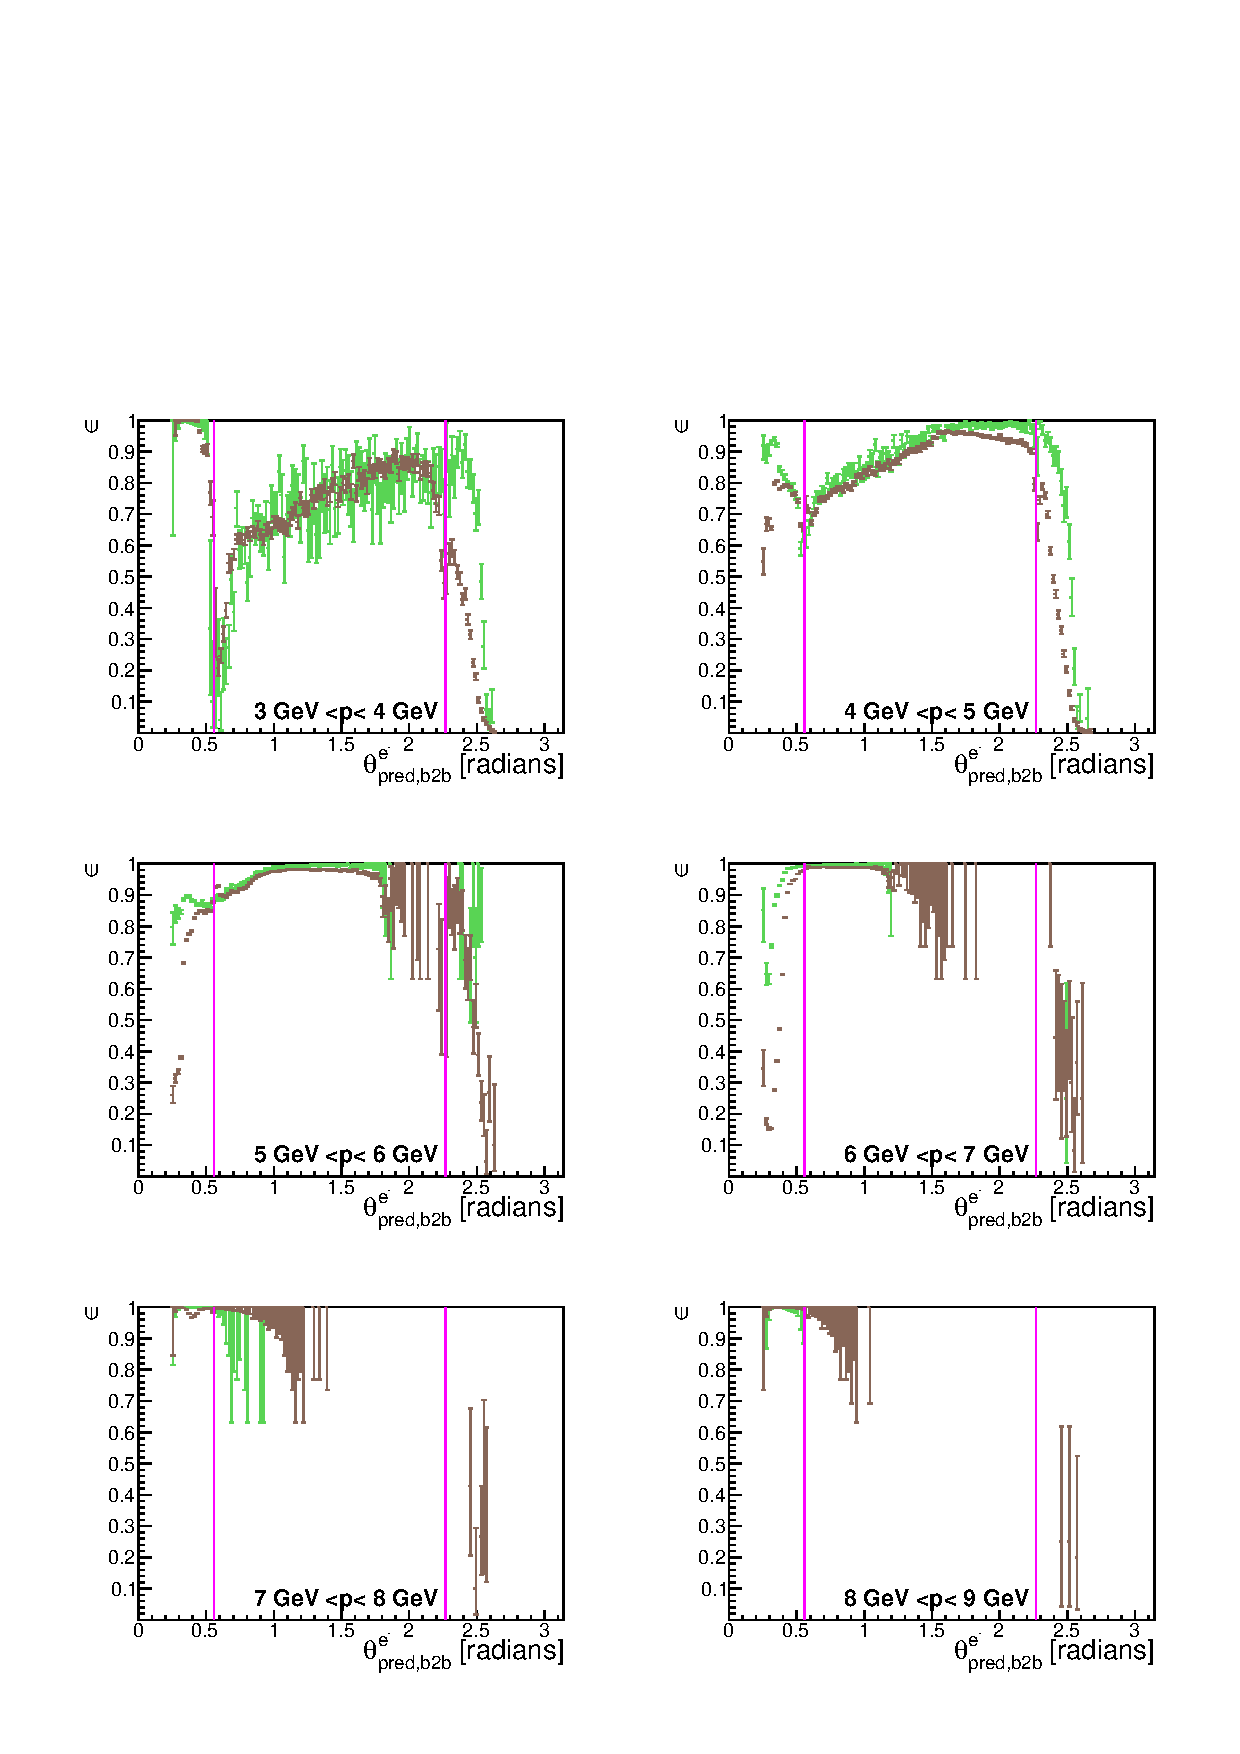
\includegraphics[width=\textwidth]{Plots/master/xPMThetaem}
	\caption[Momentum $\theta$ Electron Efficiency Phase2]{Electron $\theta$ momentum tracking efficiency plots. The tracking efficiency for phase2 data is shown in blue and phase2 MC in red. The pink line indicates the different sectors of the ECL.}
	
	\label{plt:xPMThetaem}
\end{figure}

\begin{figure}[!htbp]
	\centering
	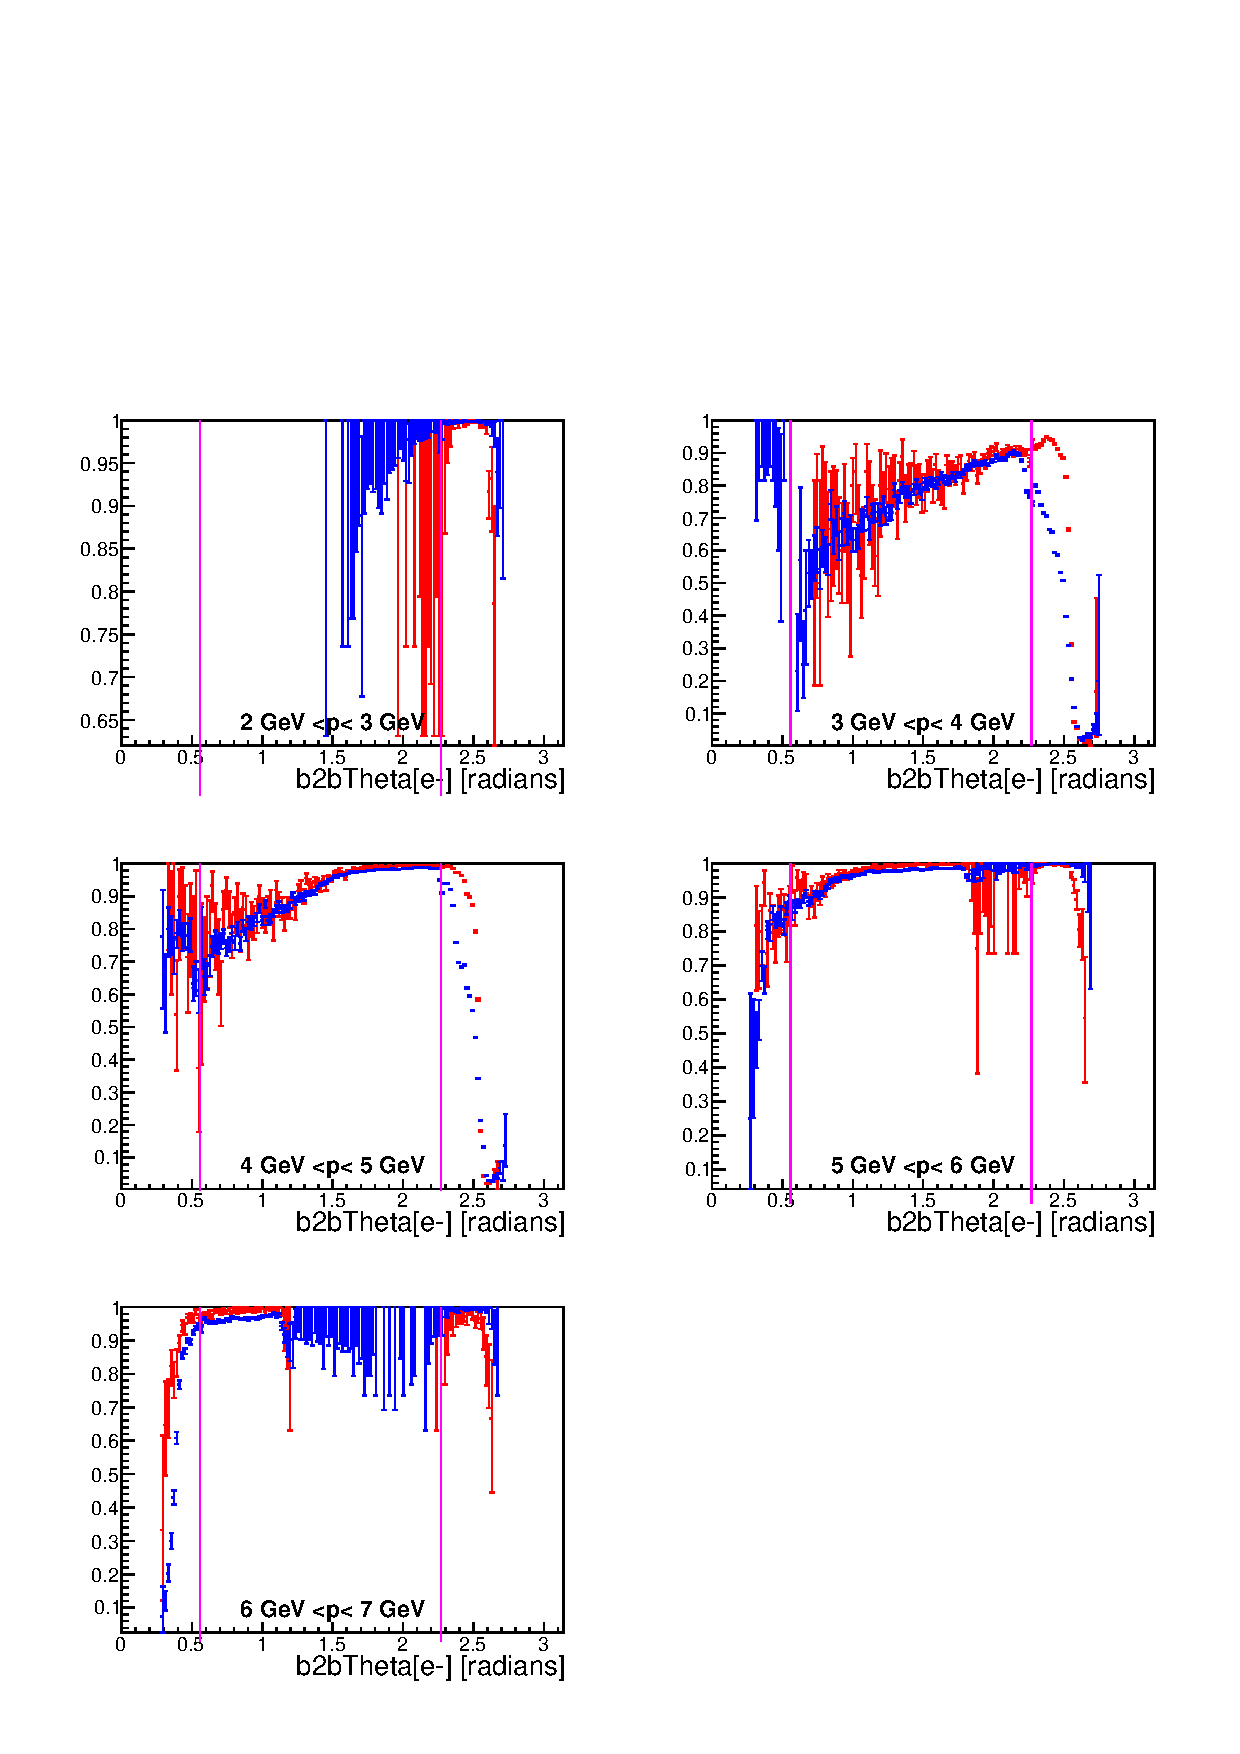
\includegraphics[width=\textwidth]{Plots/master/xPMThetaep}
	\caption[Momentum $\theta$ Positron Efficiency Phase2]{Positron $\theta$ momentum tracking efficiency plots. The tracking efficiency for phase2 data is shown in blue and phase2 MC in red. The pink line indicates the different sectors of the ECL.}
	\label{plt:xPMThetaep}
\end{figure}



\clearpage

\newpage




\section{Transverse Momentum Efficiencies}

\subsection{Forward End-Cap}

In figure \ref{plt:xPtMPhiemFC} you can see the calculated tracking efficiency for electrons in the forward end-cap  with different transverse momenta. 
For transverse momenta between $1\,\textrm{GeV}$ and $2\,\textrm{GeV}$, the biggest differences between phase2 MC and phase2 data occur at $\textrm{abs}(\phi) \gtrsim 1$. For these angles the phase2 data efficiency is noticeably worse compared to phase2 MC. The phase2 data tracking efficiency is between 0.4 and 0.95 and between 0.4 and 1 for phase2 MC. 
For transverse momenta between $2\,\textrm{GeV}$ and $3\,\textrm{GeV}$, the tracking efficiency for phase2 MC stays above 0.9 for all values of $\phi$. For phase2 data, the structure of the tracking efficiency looks more random. The lowest efficiency of approximately 0.65 occurs at $\textrm{abs}(\phi) \approx 3$ and the highest efficiency with $0.9$ at $\phi \approx 0$. Also, the efficiency has a lot of local minimums and maximums. 
For transverse momenta between $3\,\textrm{GeV}$ and $4\,\textrm{GeV}$, phase2 MC has an efficiency of over 0.97 for almost all values of $\phi$. The tracking efficiency for phase2 data also has an efficiency of over 0.97 for most $\phi$ values with the exceptions of $\textrm{abs}(\phi) \approx 0.5$, $\phi  \approx 1$ and $\phi \approx 2.9$. In all of these cases the tracking efficiency drops down significantly and in the $\phi \approx 0.5$ case even down to 0.92.

\begin{figure}[!htbp]
	\centering
	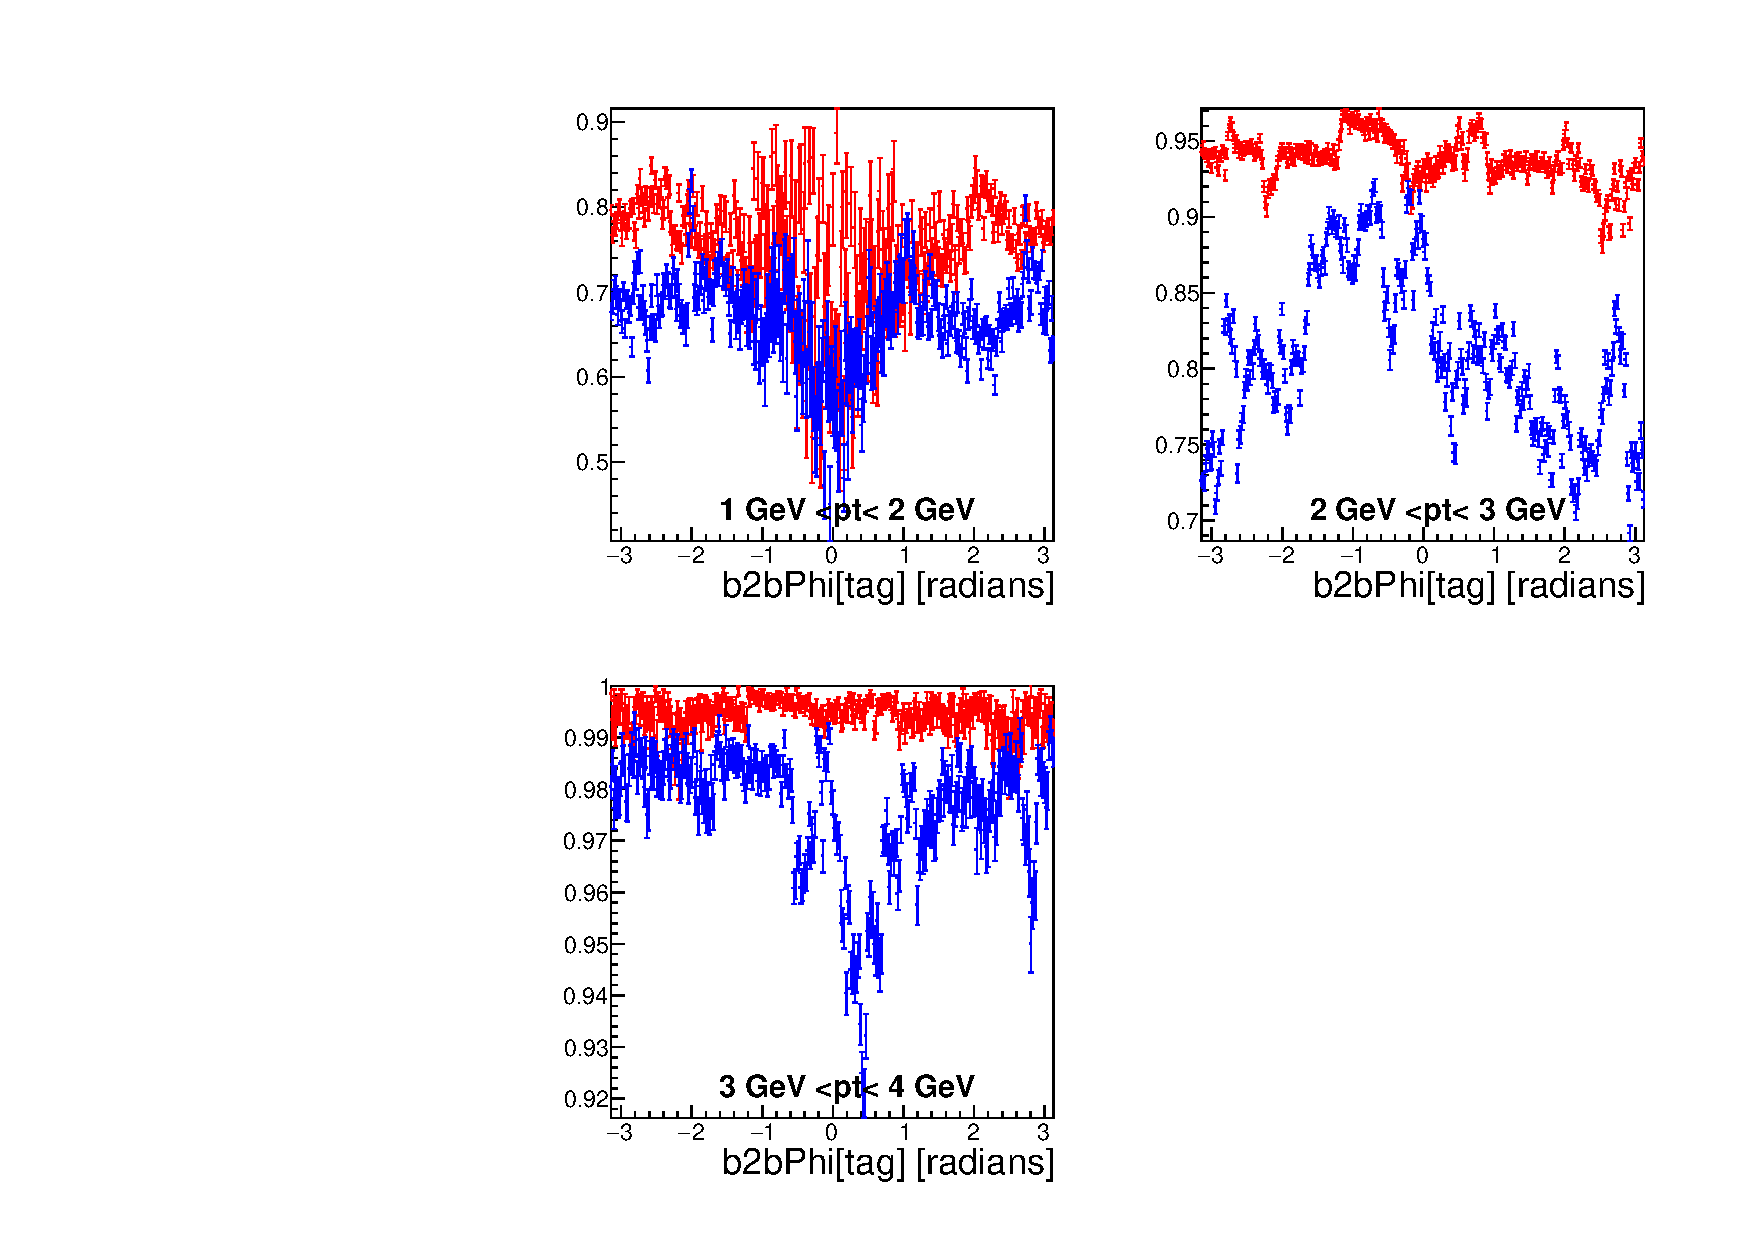
\includegraphics[width=\textwidth]{Plots/master/xPtMPhiemFC}
	\caption[Transverse Momentum $\phi$ Electron Forward End-Cap Efficiency Phase2]{Electron $\phi$ transverse momentum tracking efficiency plots in the forward end-cap. The tracking efficiency for phase2 data is shown in blue and phase2 MC in red.
		\label{plt:xPtMPhiemFC}}
\end{figure}



\newpage



\subsection{Barrel}

Figure \ref{plt:xPtMPhiemBarrel} shows the calculated phase2 electron tracking efficiency for different transverse momenta in the barrel. For transverse momenta between $2\,\textrm{GeV}$ and $3\,\textrm{GeV}$, the tracking efficiency of phase2 MC and phase2 data has a very similar structure. In both cases the lowest tracking efficiency occurs at $\phi \approx 0$. 
For transverse momenta between $3\,\textrm{GeV}$ and $5\,\textrm{GeV}$, the structure of the efficiency of phase2 MC and phase2 data differ. For phase2 MC the tracking efficiency is above 0.92 and for phase2 data above 0.91. The tracking efficiency becomes higher with increasing transverse momentum. The highest tracking efficiency occurs at transverse momenta between $5\,\textrm{GeV}$ and $6\,\textrm{GeV}$. The efficiency of phase2 MC and phase2 data never falls below 0.95. 
For phase2 data, the lowest tracking efficiency appears at $\phi \approx 0$. The error bars for phase2 MC are smaller for $\phi \approx 0$ due to the kinematics at Belle II. The electron and positron beams are hitting each other under an angle and therefore there is more statistics at $\phi \approx 0$.


Figure \ref{plt:xPtMPhiepBarrel} shows positrons tracking efficiencies in the barrel for different transverse momenta. 
For transverse momenta between $3\,\textrm{GeV}$ and $4\,\textrm{GeV}$, the calculated tracking efficiency is above 0.94 for both phase2 MC and phase2 data. The error bars are too big the see a structure in the efficiency for phase2 MC. The tracking efficiency for phase2 data is lower compared to phase2 MC for almost all values of $\phi$. There are also some noticeable dips in the efficiency at $\phi \approx -2.2$, $ \lesssim 0$, $ \approx 0.5$ and $ \approx 2.2$. 
For transverse momenta between $4\,\textrm{GeV}$ and $5\,\textrm{GeV}$, the structure of the phase2 data efficiency looks similar to the structure of the lower transverse momenta with the exception that the tracking efficiency is overall higher with at least 0.96 and the dips on phase2 data are not that dominant. 
For transverse momenta between $5\,\textrm{GeV}$ and $6\,\textrm{GeV}$, the phase2 data tracking efficiency is almost always above 0.96. Again, there is a small dip at $\phi \approx 0.5$. For phase2 MC the tracking efficiency is almost always above 0.95. 






\begin{figure}[!htbp]
	\centering
	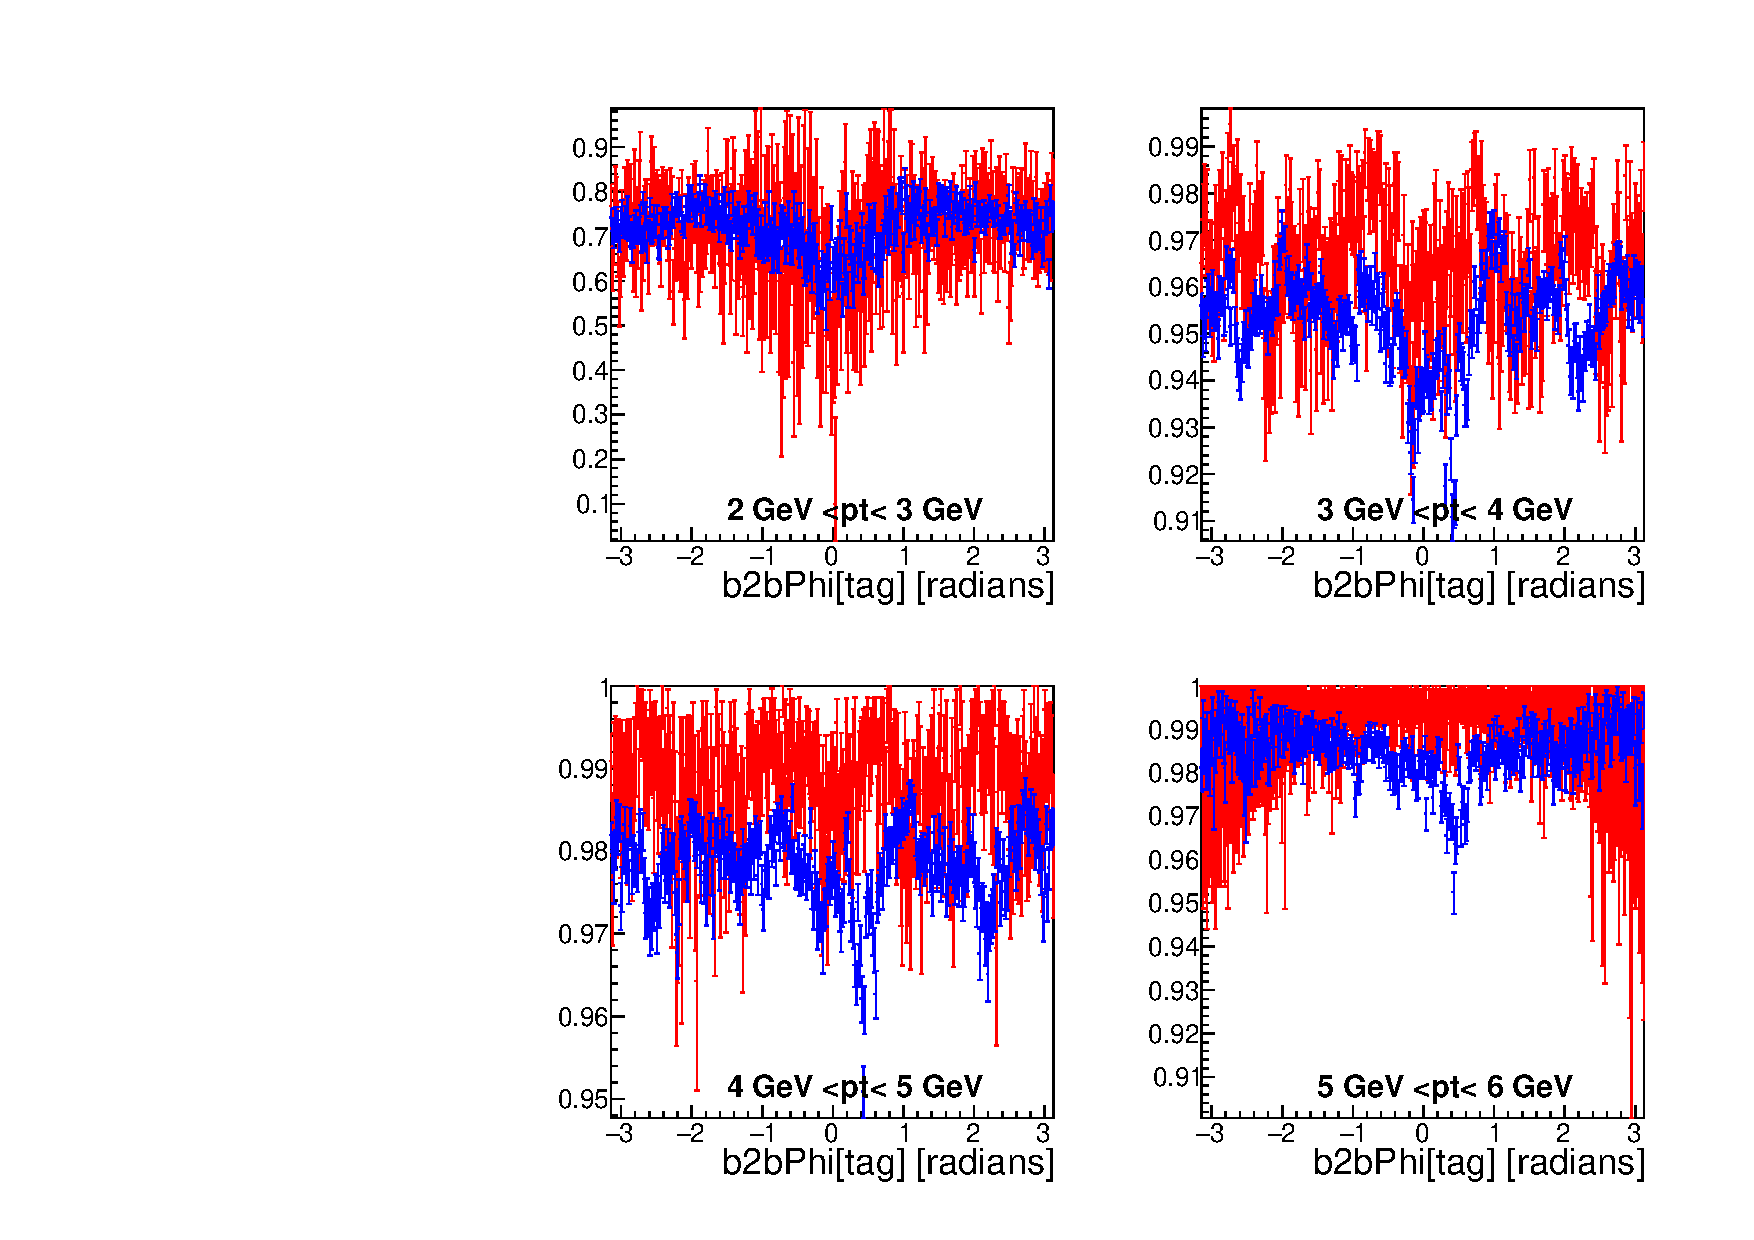
\includegraphics[width=\textwidth]{Plots/master/xPtMPhiemBarrel}
	\caption[Transverse Momentum $\phi$ Electron Barrel Efficiency Phase2]{Electron $\phi$ transverse momentum tracking efficiency plots in the barrel. The tracking efficiency for phase2 data is shown in blue and phase2 MC in red.
	\label{plt:xPtMPhiemBarrel}	}
\end{figure}




\begin{figure}[!htbp]
	\centering
	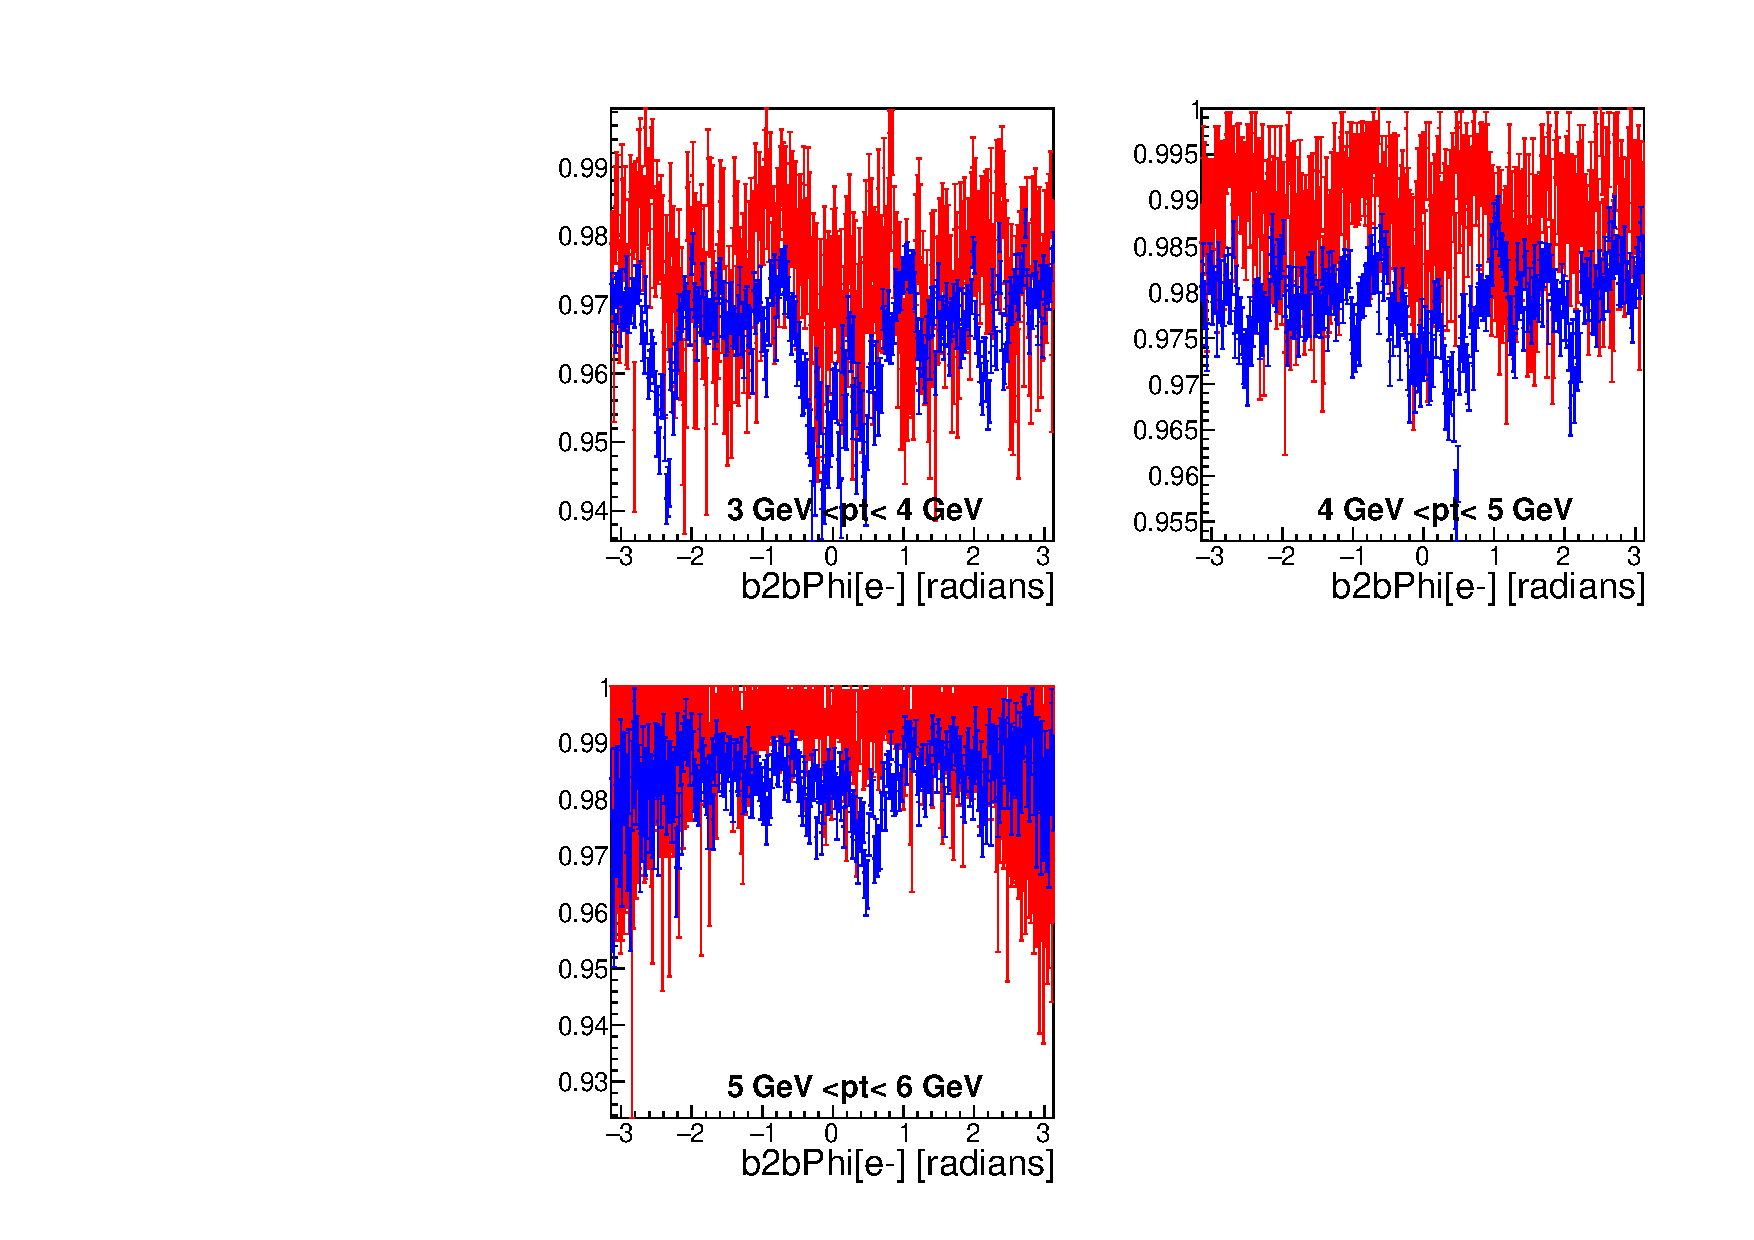
\includegraphics[width=\textwidth]{Plots/master/xPtMPhiepBarrel}
	\caption[Transverse Momentum $\phi$ Positron Barrel Efficiency Phase2]{Positron $\phi$ transverse momentum tracking efficiency plots in the barrel. The tracking efficiency for phase2 data is shown in blue and phase2 MC in red.
		\label{plt:xPtMPhiepBarrel}	}
\end{figure}




\newpage





\subsection{Backward End-Cap}


Figure \ref{plt:xPtMPhiepEC} shows the calculated positron tracking efficiencies for different transverse momenta in the backward end-cap. 
For transverse momenta between $1\,\textrm{GeV}$ and $2\,\textrm{GeV}$, the tracking efficiency of phase2 MC and phase2 data are very close together. You can see some sort of plateau at $\textrm{abs}(\phi) \lesssim 1.5$. Here, the tracking efficiency is very high compared to the efficiency of the remaining $\phi$ angles. One half of the backward end-cap appears to have a significantly better efficiency. It is also worth noting, that for $\phi <1.5$, phase2 data appears to have a higher efficiency compared to phase2 MC and for $\phi > 1.5$ it is the other way around. 
For transverse momenta between $2\,\textrm{GeV}$ and $3\,\textrm{GeV}$, the tracking efficiency for $\textrm{abs}(\phi) >1.5$ is again very low with just about 0.6. The plateau we saw before is also way more narrow and it only appears on phase2 MC. For phase2 data the tracking efficiency oscillates heavily at $\phi \approx 0$. It starts with a drop of the efficiency down to 0.4 at $\phi \approx -0.5$ followed by a local maximum of $\sim 0.9$ at $\phi \lesssim 0$. At $\phi \approx 0 $ the efficiency falls down to 0.6 and goes back up to $\sim 0.9$ at $\phi \gtrsim 0$. Finally, it falls back down to around 0.4 at $\phi \approx 0.5$. The last efficiency drop for phase2 data appears at $\phi \approx 2$. Here the efficiency falls down to $\sim 0.3$. 
For transverse momenta between $3\,\textrm{GeV}$ and $4\,\textrm{GeV}$, the calculated tracking efficiency for phase2 MC is above 0.98 for all values of $\phi$. For phase2 data, the tracking efficiency is above 0.95 for $\textrm{abs}(\phi) > 1$, but you can see the structure in the efficiency we saw in the previous transverse momenta range again. This time, the drops of the efficiency is not as dominant and it never falls below 0.87.




\begin{figure}[!htbp]
	\centering
	\includegraphics[width=\textwidth]{Plots/master/xPtMPhiepEC}
	\caption[Transverse Momentum $\phi$ Positron Backward End-Cap Efficiency Phase2]{Positron $\phi$ transverse momentum tracking efficiency plots in the backward end-cap. The tracking efficiency for phase2 data is shown in blue and phase2 MC in red.
		\label{plt:xPtMPhiepEC}	}
\end{figure}

\newpage











\subsection{$\theta$ Efficiencies}


Figure \ref{plt:xPtMThetaem} shows the calculated electron tracking efficiencies for different transverse momenta as a function of the polar angle $\theta$. For transverse momenta between $1\,\textrm{GeV}$ and $2\,\textrm{GeV}$, almost all electrons are detected in the forward end-cap.  The tracking efficiency for phase2 data is very low with only about 0.3 at $\theta \approx 0.25$. Then it jumps up to 0.75 at $\theta \approx 0.3$. After this it increases further until it reaches its maximum of about 0.9 at $\theta \approx 0.5$. The tracking efficiency for phase2 MC starts high with 0.9 at $\theta \approx 0.25$ but it first falls down to 0.7 at $\theta \approx 0.3$. After this it immediately jumps back up to 0.9. Then, it falls back to 0.8 at $\theta \approx 0.4$ and after this it rises back up to over 0.9 at $\theta \approx 0.5$.
For transverse momenta between $2\,\textrm{GeV}$ and $3\,\textrm{GeV}$, the tracking efficiency of phase2 data starts with 0.7 at $\theta \approx 0.25$. It reaches its local minimum of 0.4 at $\theta \approx 0.3$. After this the efficiency increases and has a maximum of over 0.9 at $\theta \approx 0.5$. With increasing values of $\theta$ the efficiency falls down. First rapidly in the forward end-cap then slowly in the barrel. It reaches a local minimum of 0.6 at $\theta \approx 1.0$. The tracking efficiency of phase2 MC starts with 0.85 and reaches a local maximum of 0.95 at $\theta \approx 0.5$. Similar to phase2 data, it falls down after this and reaches a local minimum of 0.6 at $\theta \approx 1.0$. In the backward end-cap, the tracking efficiency of phase2 MC starts with 0.9 and falls down rapidly to 0 at $\theta \approx 2.6$. The tracking efficiency of phase2 data has a similar structure but it is lower by about 0.4. Therefore, it reaches 0 earlier.
For transverse momenta between $3\,\textrm{GeV}$ and $4\,\textrm{GeV}$, the tracking efficiency for both phase2 MC and phase2 data start with almost 1 in the forward end-cap. They are close together and they decrease a little with increasing $\theta$. Starting at $\theta \approx 0.7$, both tracking efficiencies fall down rapidly and they both reach a local minimum of 0.7 at $\theta \approx 1.0$. After this, the phase2 data tracking efficiency gets back up slowly reaching a local maximum at $\theta \approx 2.0$. After this maximum, the efficiency of phase2 data falls down and even has a dip at the transition between the barrel and the backward end-cap. Phase2 MC on the other hand, stays more or less the same in the middle region of the barrel. But it also has a local maximum starting at $\theta \approx 2.0$. The tracking efficiency starts to fall down at $\theta \approx 2.3$.
For transverse momenta between $4\,\textrm{GeV}$ and $5\,\textrm{GeV}$, most electron only hit the barrel and the forward end-cap. the tracking efficiency of phase2 data in the forward end-cap is always above 0.9. The efficiency for phase2 MC is worse for some values of $\theta$ due to the large errors. In the barrel, both tracking efficiencies stay above 0.95 with the exception of a wide local minimum of 0.9 at $\theta \approx 1.3$. Also, the tracking efficiency for phase2 data is almost always a little worse than the tracking efficiency of phase2 MC.
For transverse momenta between $5\,\textrm{GeV}$ and $6\,\textrm{GeV}$, almost all electrons are detected in the barrel. Except for some $\theta$ angles, the tracking efficiency for phase2 MC and phase2 data stays above 0.96. The tracking efficiency of phase2 data is always a little lower than the phase2 MC tracking efficiency. 


Figure \ref{plt:xPtMThetaep} shows the calculated positron tracking efficiency for different transverse momenta as a function of the polar angle $\theta$. For transverse momenta between $1\,\textrm{GeV}$ and $2\,\textrm{GeV}$, most of the positrons are detected in the backward end-cap. The tracking efficiency of phase2 data is about 0.85 before it falls down at the end of the backward end-cap. The tracking efficiency for phase2 MC has a similar structure but is also a little higher.
For transverse momenta between $2\,\textrm{GeV}$ and $3\,\textrm{GeV}$, the tracking efficiency for phase2 data starts low  but it increases rapidly until it reaches a local maximum of about 0.85 at $\theta \approx 0.5$. After this, the tracking efficiency falls back down. It has  a local minimum of about 0.6 at $\theta \approx 1.0$. For $\theta \approx 2.0$ the tracking efficiency is over 0.9 but it falls down with increasing $\theta$ and it has a significant dip at the barrel and backward end-cap transition. Then it goes back up until it finally falls down to 0 at the end of the backward end-cap. The phase2 MC tracking efficiency has a similar structure. But the calculated tracking efficiency of phase2 MC is higher compared to phase2 data for almost all values of $\theta$. Also, the dip of the efficiency at the transition between barrel and backward end-cap is not as dominant in phase2 MC.
For transverse momenta between $3\,\textrm{GeV}$ and $4\,\textrm{GeV}$, the tracking efficiency for phase2 data starts with 0.9 at $\theta \approx 0.5$ and rises to a local maximum of 0.95 at the forward end-cap and barrel transition. After this, the tracking efficiency falls down and reaches a local minimum at $\theta \approx 1.0$. Then, it slowly increases until it reaches an efficiency of over 0.95 at $\theta \approx 2.1$. The efficiency stays at this value until the transition between the barrel and the backward end-cap. Here, it falls down a little and the efficiency reaches a local minimum of 0.88 in the backward end-cap at $\theta \approx 2.4$. Finally, the efficiency goes back up to over 0.99. The tracking efficiency for phase2 MC follows a similar path. With the exception that it starts in the forward end-cap at a higher value of over 0.95. Also, there is no local minimum for phase2 MC in the backward end-cap. But it appears to fall down at the end of the backward end-cap.
For transverse momenta between $4\,\textrm{GeV}$  and $5\,\textrm{GeV}$, the tracking efficiency for phase2 MC and phase2 data are close together. In the barrel, both are constantly above 0.92 with a wide minimum at $\theta \approx 1.0$. At $\theta \approx 2.0$, the tracking efficiency even reaches above 0.98 for both phase2 data and phase2 MC. In the backward end-cap, the tracking efficiency of phase2 MC appears to fall down earlier than the phase2 data tracking efficiency.
For transverse momenta between $5\,\textrm{GeV}$ and $6\,\textrm{GeV}$, almost all positrons hit the barrel. The tracking efficiency for both phase2 data and phase2 MC stays above 0.95 for all values with high statistic.


\begin{figure}[!htbp]
	\centering
	\includegraphics[width=\textwidth]{Plots/master/xPtMThetaem}
	\caption[Transverse Momentum $\theta$ Electron Efficiency Phase2]{Electron $\theta$ transverse momentum tracking efficiency plots. The tracking efficiency for phase2 data is shown in blue and phase2 MC in red. The pink line indicates the different sectors of the ECL.}
	\label{plt:xPtMThetaem}
\end{figure}


\begin{figure}[!htbp]
	\centering
	\includegraphics[width=\textwidth]{Plots/master/xPtMThetaep}
	\caption[Transverse Momentum $\theta$ Positron Efficiency Phase2]{Positron $\theta$ transverse momentum tracking efficiency plots. The tracking efficiency for phase2 data is shown in blue and phase2 MC in red. The pink line indicates the different sectors of the ECL.}
	\label{plt:xPtMThetaep}
\end{figure}

\newpage

\section{$\theta$-$\phi$ Efficiencies}
\label{sec:tpEff}

In figure \ref{plt:xCEff} you can see the $\theta$-$\phi$ efficiencies for phase2 MC on the left and phase2 data on the right. The efficiencies for electrons are shown in the first line and positrons in the second line. These plots combine all momenta of the particles. For electrons, there is a difference between phase2 MC and phase2 data in the forward end-cap. For phase2 MC, there is almost no drop of the efficiency in the forward end-cap in contrast to phase2 data. For positrons the differences occur in the backward end-cap. The transition between high and low tracking efficiency is way more sharp on phase2 MC compared to phase2 data. Also, at around $\phi \approx 0$ and $\theta \approx 2.4$ there is something like a \textit{horn} structure in phase2 data. This structure we already saw in section \ref{sec:MEC} for positrons with momenta between $3\,\textrm{GeV}$ and $5\,\textrm{GeV}$.




\begin{figure}[!htbp]
	\centering
	\includegraphics[width=\textwidth]{Plots/master/xCEffTP_MCData.pdf}
	\caption[$\theta$-$\phi$ Efficiency Plots Phase2]{$\theta$-$\phi$ efficiencies for phase2. Left: Phase2 MC. Right: Phase2 data. First line: electron efficiencies. Second line: positron efficiencies. The 2D plots with the corresponding error can be found in the appendix \ref{plt:xCEff_Error}. The pink line indicates the different sectors of the ECL.}
	\label{plt:xCEff}
\end{figure}


\chapter{Phase3 Tracking Efficiency}
\label{chp:TrackingEfficiencyPhase3}

\lettrine{T}{h}is chapter will start with a short description of phase3. Then the location of the files taken into account will be provided. Finally, the calculated tracking efficiency of electrons and positrons will be presented.

\section{Phase3}
\label{sec:P3}

Phase3 started successfully on March 11th, 2019. In contrast to phase2 the whole SVD and all ladders of the innermost in addition to two ladders of the outermost layer of the PXD were installed during phase3. A sketch of the PXD arrangement is shown in the appendix figure \ref{fig:phase3pxd}. Phase3 is the first physics run of the Belle II project, in which the Belle II experiment will take data in a mostly fully equipped detector.\cite{phase3}



\section{Location}

To have as much events as possible, all phase3 data files are taken into account. They contain Experiment 7 located on KEKCC at:

/group/belle2/dataprod/Data/release-03-02-02/DB00000654/proc9/e0007/4S/
r0*/all/mdst/sub00/*.root
\newline 

and Experiment 8 located on KEKCC at:


/group/belle2/dataprod/Data/release-03-02-02/DB00000654/proc9/e0008/4S/
r0*/all/mdst/sub00/*.root
\newline


For Monte Carlo we will consider all files located on KEKCC at:




/belle/MC/release-01-00-02/DB00000294/MC10/prod00004664/s00/e0000/4S/
r00000/3600520000/mdst/sub00
\newline

The selection described in chapter \ref{chap:Phase2Eff} will be used to select Bhabha events.



\begin{figure}[h!]
	\includegraphics[width=\textwidth]{Plots/master3/CCandP3.pdf}
	\caption[Total Number Of Events After The Selection Phase3]{The number of candidates per event after the selection is shown. Left: Phase3 Data. Right: Phase3 MC. A total of 852093 candidates are selected for phase3 data and $5.344275\cdot10^7$ candidates are selected for phase2 MC.}
	\label{fig:nCandAS3}
\end{figure}

In figure \ref{fig:nCandAS3} you can see the number of selected virtual photon candidates per event. You can see that in both phase3 MC and phase3 data only one candidate is selected per event.










\newpage

\section{Tracking Efficiency}

In this section the calculated tracking efficiencies for phase3 will be presented.  Phase3 data will be shown in brown together with phase3 MC in green. The individual tracking efficiencies can be found in the appendix chapter \ref{A:3}. Just like chapter \ref{chp:TrackingEfficiencyPhase2}, only efficiencies with $\Delta \epsilon < 0.4$ are plotted.


\subsection{Momentum Efficiencies}


\subsubsection{Forward End-Cap}

Figure \ref{plt:xPMPhiemFC3} shows the calculated electron tracking efficiency for different momenta in the forward end-cap.
For momenta between $4\,\textrm{GeV}$ and $5\,\textrm{GeV}$, the tracking efficiency for phase3 data starts at 0.85 and falls down until it reaches a minimum of 0.7 at $\phi \approx 0$. After this it goes back up to 0.85. At the minimum something strange is happening to the phase3 data tracking efficiency. It seems like the tracking efficiency drops by $\sim 0.1$ every other value of $\phi$. The result are two \textit{ribbons} of efficiency in this region. The tracking efficiency of phase3 MC has a similar structure but due to the lower statistics the error bars are way bigger.
For momenta between $5\,\textrm{GeV}$ and $6\,\textrm{GeV}$, the structure of the tracking efficiencies are similar to the ones of the previous momentum range. But this time, the tracking efficiency starts at 0.9 for phase3 data and an efficiency of about 0.82 is reached in the minimum at $\phi \approx 0$. Also, for this momentum range, there are no \textit{ribbons} of efficiency in the minimum.
For momenta between $6\,\textrm{GeV}$ and $7\,\textrm{GeV}$, the tracking efficiency for phase3 MC stays above 0.95 for almost all values of $\phi$. The tracking efficiency for phase3 data ranges between 0.89 and 0.98. Some efficiencies appear to be scattered more or less random in this range.
For momenta between $7\,\textrm{GeV}$ and $8\,\textrm{GeV}$, the tracking efficiency for phase3 data is almost 1 for $\textrm{abs}(\phi) > 1.5$. For $\textrm{abs}(\phi) < 1.5$, the tracking efficiency varies between 0.99 and 1. The phase3 MC tracking efficiency ranges between 0.975 and 1 for most values of $\phi$. The error bars are significantly larger for $\textrm{abs}(\phi) > 1.5$.
The best electron tracking efficiency for phase3 in the forward end-cap is obtained for electrons with a momentum between $7\,\textrm{GeV}$ and $8\,\textrm{GeV}$.



\begin{figure}[!htbp]
	\centering
	\includegraphics[width=\textwidth]{Plots/master3/xPMPhiemFCP3}
	\caption[Momentum $\phi$ Electron Forward End-Cap Efficiency Phase3]{Electron $\phi$ tracking efficiency plots in the forward end-cap. The tracking efficiency for phase3 data is shown in brown and phase3 MC in green.}
	\label{plt:xPMPhiemFC3}
\end{figure}



\newpage
\subsubsection{Barrel}

Figure \ref{plt:xPMPhiemBarrel3} shows the electron tracking efficiencies in the barrel.
For momenta between $4\,\textrm{GeV}$ and $5\,\textrm{GeV}$, the phase3 MC tracking efficiency is between 0.75 and 0.95. For phase3 data the tracking efficiency is between $ \sim 0.80$ and 0.92. The lowest efficiencies occurs at $\phi \approx 0$, the highest efficiencies at $\textrm{abs}(\phi) \approx \pi$.
The tracking efficiencies for higher momenta have a similar structure. 
For momenta between $5\,\textrm{GeV}$ and $6\,\textrm{GeV}$ the tracking efficiency is between $\sim 0.90$ and $\sim 0.99$ for phase3 MC and between $\sim 0.93$ and 0.98. The best tracking efficiency appears at momenta between $6\,\textrm{GeV}$ and $7\,\textrm{GeV}$. Here, the calculated tracking efficiency is between $\sim 0.98$ and 1 for phase3 MC and between 0.990 and 0.997 for phase3 data.

Figure \ref{plt:xPMPhiepBarrel3} shows the positron tracking efficiency in the barrel. 
For momenta between $3\,\textrm{GeV}$ and $4\,\textrm{GeV}$, the calculated tracking efficiency for phase3 MC is between $\sim 0.7$ and $\sim 0.97$. The lowest efficiency  occurs at $\phi \approx 0$ and the highest at $\textrm{abs}(\phi) \approx \pi$. The phase3 data has a similar structure but the efficiency is between $\sim 0.8$ and $\sim 0.9$.
For momenta between $4\,\textrm{GeV}$ and $5\,\textrm{GeV}$, the tracking efficiency is between $\sim 0.965$ and 0.998 for phase3 MC and between 0.98 and 0.990. The structure of the efficiencies is similar to the previous momenta but not as dominant.
For momenta between $5\,\textrm{GeV}$ and $6\,\textrm{GeV}$, the tracking efficiency is between $\sim 0.94$ and 1 for phase3 MC and between $\sim 0.97$ and $\sim 0.99$ for phase3 data. The structure of the efficiency of phase3 data is different to the structure of the efficiency for lower momenta. Now, the highest efficiency occurs at $\phi \approx 0$ and the lowest efficiency at $\textrm{abs}{(\phi)} \approx \pi$.
For momenta between $6\,\textrm{GeV}$ and $7\,\textrm{GeV}$, the calculated positron tracking efficiency is  between $\sim 0.8$ and 1 for phase3 MC and between $\sim 0.95$ and 0.98 for phase3 data. The efficiency distribution is rather flat in both cases.

\begin{figure}[!htbp]
	\centering
	\includegraphics[width=\textwidth]{Plots/master3/xPMPhiemBarrelP3}
	\caption[Momentum $\phi$ Electron Barrel Efficiency Phase3]{Electron $\phi$ tracking efficiency plots in the barrel. The tracking efficiency for phase3 data is shown in brown and phase3 MC in green.}
	\label{plt:xPMPhiemBarrel3}
\end{figure}




\begin{figure}[!htbp]
	\centering
	\includegraphics[width=\textwidth]{Plots/master3/xPMPhiepBarrelP3}
	\caption[Momentum $\phi$ Positron Barrel Efficiency Phase3]{Positron $\phi$ tracking efficiency plots in the barrel. The tracking efficiency for phase3 data is shown in brown and phase3 MC in green.}
	\label{plt:xPMPhiepBarrel3}
\end{figure}













\newpage

\subsubsection{Backward End-Cap}

Figure \ref{plt:xPMPhiepEC3} shows the positron tracking efficiency in the backward end-cap.
For momenta between $2\,\textrm{GeV}$ and $3\,\textrm{GeV}$, the phase3 MC tracking efficiency is above 0.9 for most values of $\phi$. The biggest error bars appear at $\phi \approx 0$. For phase3 data, the tracking efficiency is above 0.99 for all values of $\phi$.
For momenta between $3\,\textrm{GeV}$ and $4\,\textrm{GeV}$, the tracking efficiency of phase3 MC is between $\sim 0.9$ and 1. Again, the lowest efficiency occurs at $\phi \approx 0$ and the highest efficiency at $\textrm{abs}(\phi) \approx \pi$. The tracking efficiency of phase3 data has a strange structure. It is scattered between 0.75 and 0.97 but the error bars are rather small. Most of the time, the efficiency is above 0.9 but the efficiency drops by over 0.1 every other value of $\phi$.
For momenta between $4\,\textrm{GeV}$ and $5\,\textrm{GeV}$, the tracking efficiency for phase3 MC is between 0.96 and 1. Similar to the previous momenta range, the lowest tracking efficiency occurs at  $\phi \approx 0$ and the highest efficiency at $\textrm{abs}(\phi) \approx \pi$. The tracking efficiency structure for phase3 data is also similar to the previous momenta range. But for this momenta range, the tracking efficiency is between 0.9 and $\sim 0.99$ and without the scattered tracking efficiency values, the efficiency would be around 0.98. Also for this momenta range, the number of efficiency drops is smaller compared to the previous momenta range.
For momenta between $5\,\textrm{GeV}$ and $6\,\textrm{GeV}$, the tracking efficiency for phase3 MC is between 0.6 and 1. But the error bars are very large and therefore a structure in the efficiency can not be determined. For phase3 data, the tracking efficiency is above 0.9 for almost all values of $\phi$.




\begin{figure}[!htbp]
	\centering
	\includegraphics[width=\textwidth]{Plots/master3/xPMPhiepECP3}
	\caption[Momentum $\phi$ Positron Backward End-Cap Efficiency Phase3]{Positron $\phi$ tracking efficiency plots in the backward end-cap. The tracking efficiency for phase3 data is shown in brown and phase3 MC in green.}
	
	\label{plt:xPMPhiepEC3}
\end{figure}






\newpage

\subsubsection{$\theta$ Efficiencies}



In figure \ref{plt:xPMThetaem3} you can see the calculated electron tracking efficiency as a function of the polar angle $\theta$.
For momenta between $3\,\textrm{GeV}$ and $4\,\textrm{GeV}$ the tracking efficiency for phase3 MC starts in the forward end-cap with over 0.95 for most $\phi$ values. At the forward end-cap and barrel transition the efficiency drops down to 0 and goes back up to 0.6 at $\theta \approx 0.7$. After this, the tracking efficiency slowly increases to between $\sim 0.80$ and $\sim 0.95$ at $\theta \approx 0.4$. Then the efficiency drops drastically down to 0. The tracking efficiency of phase3 data starts even higher with almost 1 in the forward end-cap. Similar to the tracking efficiency of phase3 MC, the phase3 data efficiency drops at the forward end-cap and barrel transition. After this, the efficiency follows the phase3 MC efficiency until $\theta \approx 2.2$. At the barrel and backward end-cap transition, the phase3 data tracking efficiency drops down to around 0.55. In the backward end-cap the efficiency goes back up 0.7 before it finally falls down to 0.
For momenta between $4\,\textrm{GeV}$ and $5\,\textrm{GeV}$, both the phase3 MC and phase3 tracking efficiency starts at around 0.95 and decline with increasing $\theta$. A local minimum of $\epsilon \approx 0.6$ appears at the forward end-cap transition. After the transition the efficiency jumps back to around 0.75 and then increases slowly until $\theta \approx 1.5$. Here the tracking efficiency stops for phase3 MC and it stays at the same height for the rest of the barrel. The tracking efficiency for phase3 MC finally drops down to 0 in the backward end-cap. In contrast, the phase3 data tracking efficiency already starts to fall down slowly at $\theta \approx 1.5$. At the barrel and backward end-cap transition, the phase3 data tracking efficiency drops down to $\sim0.8$. After this it goes back up to $\sim0.85$ and it processed to decline, until it reaches 0 at the end of the backward end-cap.
For momenta between $5\,\textrm{GeV}$ and $6\,\textrm{GeV}$, the tracking efficiency for both phase3 MC and phase3 data starts at around 0.95. They then decrease very fast until the transition between forward end-cap and barrel with a tracking efficiency of about 0.85. At this transition a peak in the tracking efficiency occurs. The tracking efficiency jumps up to about 0.95 and falls back down to $\sim 0.9$ after the transition. Then, the efficiency goes up and reaches a plateau at $\theta \approx 1.3$ with an tracking efficiency of over 0.97.
For momenta between $6\,\textrm{GeV}$ and $7\,\textrm{GeV}$, the phase3 MC and phase3 data tracking efficiency starts at around 0.95 and directly falls down to 0.9 at $\theta \approx 0.3$. After this, the tracking efficiency goes back up to almost 1 and it stays this high until $\theta \approx 1.3$.
For momenta between $7\,\textrm{GeV}$ and $8\,\textrm{GeV}$, almost all electrons hit the forward end-cap. For phase3 data the tracking efficiency starts at almost 1 and stays that high for the whole forward end-cap. The tracking efficiency for phase3 MC also starts at almost 1 but the error bars become very large very fast with increasing $\theta$.

Figure \ref{plt:xPMThetaep3} shows the positron tracking efficiency in the backward end-cap as a function of the polar angle $\theta$.
For momenta between $2\,\textrm{GeV}$ and $3\,\textrm{GeV}$, most of the positrons are detected in the backward end-cap. For phase3 MC the tracking efficiency is above 0.97 for almost all values of $\theta$ in the backward end-cap. For phase3 data, the tracking efficiency is even higher with over 0.99.
For momenta between $3\,\textrm{GeV}$ and $4\,\textrm{GeV}$, the tracking efficiency for phase3 data starts in the forward end-cap with over 0.9 but it decreases with increasing $\theta$. In the barrel, the tracking efficiency for phase3 data starts very low. Probably due to the transition between forward end-cap and barrel. The efficiency jumps up to around 0.6 at $\theta \approx 0.7$. After this the tracking efficiency slowly increases. A difference between the tracking efficiency of phase3 MC and phase3 data occurs in at the transition between the barrel and the backward end-cap and in the backward end-cap itself. Around the transition the phase3 data efficiency has a small dip while the phase3 tracking efficiency has a small peak. In the backward end-cap, the phase3 MC tracking efficiency gets higher faster than the phase3 data tracking efficiency. A cap between the two of them is created. Also, there is a another small dip in the phase3 data tracking efficiency at $\theta \approx 2.6$. 
For momenta between $4\,\textrm{GeV}$ and $5\,\textrm{GeV}$, the tracking efficiency of phase3 MC and phase3 data starts at around 0.9 and it falls down with increasing $\theta$. It reaches a minimum at the forward end-cap and barrel transition. After this transition, the tracking efficiency gets higher until $\theta \approx 1.6$. After this, the tracking efficiency continues to get bigger starting with over 0.95 and ending with almost 1 at the transition between barrel and backward end-cap. In the backward end-cap, the efficiency decreases slowly before it peaks at the very end of the backward end-cap. For phase3 data, there is even a small dip before that very last peak.
For momenta between $5\,\textrm{GeV}$ and $6\,\textrm{GeV}$, the tracking efficiency starts rather low in the forward end-cap, but in the barrel the tracking efficiency begins to rise. It reaches its plateau of $\epsilon \gtrsim 0.97$ at around $\theta \approx 1.3$. In the backward end-cap, the phase3 data tracking efficiency is noticeably higher than the phase3 tracking efficiency. Also, there is a small dip in the phase3 tracking efficiency at $\theta \approx 1.9$. 
For momenta between $6\,\textrm{GeV}$ and $7\,\textrm{GeV}$, the tracking efficiency increases in the forward end-cap from  about 0.8 to 0.95 for phase3 data and to over 0.97 for phase3 MC. In the barrel, the tracking efficiency continues to increase for phase3 data until it reaches 0.99. There is a dip in the tracking efficiency at $\theta \approx 1.1$ for phase3 data. At $\theta \approx 1.2$. The efficiency drops by over $5\,\%$. The phase3 MC tracking efficiency stays in the barrel above 0.97. In the backward end-cap, phase3 data has a tracking efficiency of over 0.98.



\begin{figure}[!htbp]
	\centering
	\includegraphics[width=\textwidth]{Plots/master3/xPMThetaemP3}
	\caption[Momentum $\theta$ Electron Efficiency Phase3]{Electron $\theta$ momentum tracking efficiency plots. The tracking efficiency for phase3 data is shown in brown and phase3 MC in green. The pink line indicates the different sectors of the ECL.}
	
	\label{plt:xPMThetaem3}
\end{figure}

\begin{figure}[!htbp]
	\centering
	\includegraphics[width=\textwidth]{Plots/master3/xPMThetaepP3}
	\caption[Momentum $\theta$ Positron Efficiency Phase3]{Positron $\theta$ momentum tracking efficiency plots. The tracking efficiency for phase3 data is shown in brown and phase3 MC in green. The pink line indicates the different sectors of the ECL.}
	\label{plt:xPMThetaep3}
\end{figure}




\newpage
\subsection{Transverse Momentum Efficiencies}





\subsubsection{Forward End-Cap}


In figure \ref{plt:xPtMPhiemFC3} you can see the calculated tracking efficiency for electrons in the forward end-cap for different transverse momenta. 
For transverse momenta between $1\,\textrm{GeV}$ and $2\,\textrm{GeV}$, the tracking efficiency for phase3 data and phase3 MC is above $\sim 0.85$ for $\textrm{abs}(\phi) >1.5$. For decreasing $\textrm{abs}(\phi)$, the efficiency also decreases with a minimum at $\phi \approx 0$. Similar to the first momentum plot of figure \ref{plt:xPMPhiemFC}\footnote{This figure shows the phase3 electron tracking efficiencies for different momenta in the forward end-cap}, there is a \textit{ribbon} structure in the phase3 data tracking efficiency at $\phi \approx 0$.
For transverse momenta between $2\,\textrm{GeV}$ and $3\,\textrm{GeV}$, the phase3 MC tracking efficiency is above 0.9 for all values of $\phi$. It has a minimum at $\phi \approx 0$ and the highest efficiencies are reached at $\phi \approx \pi$. The tracking efficiency for phase3 data is between 0.88 and 0.98. Again, some efficiencies appear to be scattered more or less random at this range. 
For transverse momenta between $3\,\textrm{GeV}$ and $4\,\textrm{GeV}$, the tracking efficiency for phase3 MC is above 0.96 for all values of $\phi$. For phase3 data, the tracking efficiency is even above 0.985 for almost all values of $\phi$. There are some exceptions which again, appears to be scattered.


\begin{figure}[!htbp]
	\centering
	\includegraphics[width=\textwidth]{Plots/master3/xPtMPhiemFCP3}
	\caption[Transverse Momentum $\phi$ Electron Forward End-Cap Efficiency Phase3]{Electron $\phi$ transverse momentum tracking efficiency plots in the forward end-cap. The tracking efficiency for phase3 data is shown in brown and phase3 MC in green.}
	\label{plt:xPtMPhiemFC3}
\end{figure}



\newpage
\subsubsection{Barrel}


Figure \ref{plt:xPtMPhiemBarrel3} shows the calculated electron tracking efficiency in the barrel for different transverse momenta.
For transverse momenta between $2\,\textrm{GeV}$ and $3\,\textrm{GeV}$, the tracking efficiency for phase3 MC the errors are rather large but you can still see that the minimum of the tracking efficiency is at $\phi \approx 0$. The tracking efficiency for phase3 data, seems to oscillate between $\sim 0.6$ and $\sim 0.8$. The two maximums appear at $\textrm{abs}(\phi) \approx 2.0$ and the two minimums at $\phi \approx o$ and $\textrm{abs}(\phi) \approx \pi$.
For transverse momenta between $3\,\textrm{GeV}$ and $4\,\textrm{GeV}$, the oscillation is still visible for phase3 data and phase3 MC. But it is not as dominant. The tracking efficiency oscillates between $\sim 0.93$ and  $\sim 0.97$ for phase3 data and between $\sim 0.90$ and $\sim 0.99$ for phase3 MC.
For transverse momenta between $4\,\textrm{GeV}$ and $5\,\textrm{GeV}$, the tracking efficiency stays rather flat for both phase3 data and phase3 MC. The efficiency is between 0.97 and 0.99 for phase3 data and between $\sim 0.95$ and $\sim 1$ for phase3 MC.
For transverse momenta between $5\,\textrm{GeV}$ and $6\,\textrm{GeV}$, the calculated tracking efficiency is between 0.98 and almost 1 for phase3 data and between $\sim 0.95$ and 1 for phase3 MC. Phase3 data has the best tracking efficiency at $\textrm{abs}(\phi) \approx \pi$ in contrast to phase3 MC which has the best tracking efficiency at $\phi \approx 0$ due to the large errors at $\textrm{abs}(\phi) \approx \pi$. 

In figure \ref{plt:xPtMPhiepBarrel3}, you can see the calculated positron tracking efficiency in the barrel for different transverse momenta.
For transverse momenta between $3\,\textrm{GeV}$ and $4\,\textrm{GeV}$, the calculated tracking efficiency is between $\sim 0.93$ and $\sim 0.99$ for phase3 MC and between $\sim 0.96$ and $\sim 0.98$ for phase3 data. Again, the lowest efficiencies occurs at $\phi \approx 0$.
For transverse momenta between $4\,\textrm{GeV}$ and $5\,\textrm{GeV}$, the calculated tracking efficiency for phase3 MC is between 0.96 and 1 and between $\sim 0.975$ and $\sim 0.988$ for phase3 data. 
For transverse momenta between $5\,\textrm{GeV}$ and $6\,\textrm{GeV}$, the tracking efficiency is between $\sim 0.985$ and $\sim 0.995$ for phase3 data and between $\sim 0.94$ and 1 for phase3 MC. The error bars for phase3 MC are decreasing in length with increasing $\textrm{abs}(\phi)$.








\begin{figure}[!htbp]
	\centering
	\includegraphics[width=\textwidth]{Plots/master3/xPtMPhiemBarrelP3}
	\caption[Transverse Momentum $\phi$ Electron Barrel Efficiency Phase3]{Electron $\phi$ transverse momentum tracking efficiency plots in the barrel. The tracking efficiency for phase3 data is shown in brown and phase3 MC in green.}
	\label{plt:xPtMPhiemBarrel3}
\end{figure}




\begin{figure}[!htbp]
	\centering
	\includegraphics[width=\textwidth]{Plots/master3/xPtMPhiepBarrelP3}
	\caption[Transverse Momentum $\phi$ Positron Barrel Efficiency Phase3]{Positron $\phi$ transverse momentum tracking efficiency plots in the barrel. The tracking efficiency for phase3 data is shown in brown and phase3 MC in green.}
	\label{plt:xPtMPhiepBarrel3}
\end{figure}





\newpage

\subsubsection{Backward End-Cap}



Figure \ref{plt:xPtMPhiepEC3} shows the calculated positron tracking efficiency in the backward end-cap for different momenta.
For transverse momenta between $1\,\textrm{GeV}$ and $2\,\textrm{Gev}$, the calculated phase3 MC tracking efficiency is above 0.92 for $\textrm{abs}(\phi) >1$. For $\textrm{abs}(\phi)<1$ the error bars are noticeably larger and the efficiency is between 0.75 and 1. For phase3 data a strange structure occurs. For phase3 data the highest tracking efficiency appears at $\textrm{abs}(\phi) <0.5$. Here the efficiency is between $\sim 0.96$ and $\sim 0.99$. For $\textrm{abs}(\phi) > 0.5$ the highest efficiency is $\sim 0.97$. And the tracking efficiencies seem to be scattered between 0.75 and 0.96.
For transverse momenta between $2\,\textrm{GeV}$ and $3\,\textrm{GeV}$, the calculated tracking efficiency is between $\sim 0.95$ and $\sim 0.99$ for phase3 MC and between $\sim 0.72$ and $\sim 0.98$ for phase3 data. Again, the tracking efficiency for phase3 data appears to be scattered randomly.
For transverse momenta between $3\,\textrm{GeV}$ and $4\,\textrm{GeV}$, the tracking efficiency for phase3 MC is between $\sim 0.96$ and 1. The efficiency range is mostly determined by the error bars. The tracking efficiency for phase3 data is above 0.99 most of the time. There are some rather smaller dips at $\phi \approx -\pi, -1.8, -1.2, -0.8, 1.2 \textrm{ and } 2.1$.



\begin{figure}[!htbp]
	\centering
	\includegraphics[width=\textwidth]{Plots/master3/xPtMPhiepECP3}
	\caption[Transverse Momentum $\phi$ Positron Backward End-Cap Efficiency Phase3]{Positron $\phi$ transverse momentum tracking efficiency plots in the backward end-cap. The tracking efficiency for phase3 data is shown in brown and phase3 MC in green.}
	
	\label{plt:xPtMPhiepEC3}
\end{figure}






\newpage

\subsubsection{$\theta$ Efficiencies}

Figure \ref{plt:xPtMThetaem3} shows the calculated electron tracking efficiency as a function of the polar angle $\theta$ for different transverse momenta.
For transverse momenta between $1\,\textrm{GeV}$ and $2\,\textrm{GeV}$, almost all electrons hit one of the end-caps. In the forward end-cap, both the phase3 MC and phase3 data tracking efficiency start at 0.95 but both fall down to $\sim 0.78$ at $\theta \approx 0.4$. After this, both efficiencies rise back up to over 0.9 at $\theta \approx 0.5$. At the forward end-cap and barrel transition, the efficiency falls down again. In the backward end-cap, the phase3 data tracking efficiency rises at first. It reaches a local maximum of about 0.8 at $\theta \approx 2.5$. For increasing $\theta$ the tracking efficiency falls down until it finally reaches 0 at the end of the backward end-cap.
For transverse momenta between $2\,\textrm{GeV}$ and $3\,\textrm{GeV}$, the calculated tracking efficiency for phase3 MC starts very high with almost 1 at the beginning of the forward end-cap. But it also falls down to $\sim 0.95$ quickly. At $\theta \approx 0.45$, the phase3 MC tracking efficiency falls down drastically to $\sim 0.7$ at the forward end-cap barrel transition. After this it slowly decreases further. The phase3 data tracking efficiency also starts very high at the beginning of the forward end-cap. But it also has a small dip at $\theta \approx 0.3$. The phase3 data tracking efficiency also falls drastically at $\theta \approx 0.45$ until it reaches the barrel. In the barrel it continuous to fall slowly. After the barrel and backward end-cap transition both the phase3 MC and the phase3 data tracking efficiency first rise to a maximum of $\sim 0.95$ for phase3 MC and $\sim 0.8$ for phase3 data at $\theta \approx 2.45$. After this maximum, both efficiencies drop.
For transverse momenta between $3\,\textrm{GeV}$ and $4\,\textrm{GeV}$, the calculated tracking efficiency in the forward end-cap is above 0.99 for both phase3 data and phase3 MC for almost all values of $\theta$. In the barrel, the phase3 data tracking efficiency starts to fall down and reaches a local minimum of about 0.72 at $\theta \approx 1.2$. After this the tracking efficiency rises slowly up to $\sim 0.85$ at $\theta \approx 2.0$. The tracking efficiency of phase3 MC also falls down in the barrel but due to the large errors the minimum is somewhere between $1.0 < \theta < 2.0$. After $\theta \approx 2.0$ both tracking efficiencies jump up and stay at roughly the same hight until $\theta \approx 2.4$. The phase3 data tracking efficiency goes up to $\sim 0.9$ and the phase3 MC efficiency goes up to over 0.95. The last maximum appears at $\theta \approx 2.45$. Here, the tracking efficiency for phase3 data goes up to over 0.96 before it  falls down at the end of the backward end-cap.
For transverse momenta between $4\,\textrm{GeV}$ and $5\,\textrm{GeV}$, the calculated phase3 data tracking efficiency is above 0.98 for almost all values of $\theta$ in the forward end-cap. At the forward end-cap and barrel transition, the tracking efficiency drops down to $\sim 0.95$. But it jumps back to almost 1 for both phase3 data and phase3 MC afterwards. Then, with increasing $\theta$, the tracking efficiency slowly falls down until it reaches its local minimum of $\sim 0.92$ at $\theta \approx 1.4$. After this minimum, the tracking efficiencies go back up. Phase3 data already reaches its efficiency plateau of $\epsilon \approx 0.95 $ at $\theta \approx 1.6$. Phase3 MC on the other hand rises up to  almost 1 at $\theta \approx 1.9$. This results in a difference of the efficiencies between phase3 data and phase3 MC.
For transverse momenta between $5\,\textrm{GeV}$ and $6\,\textrm{GeV}$, almost all electrons hit the barrel. The tracking efficiency starts with over 0.99 for both phase3 data and phase3 MC at $\theta \approx 0.9$. The phase3 tracking efficiency stays more or less the same with increasing $\theta$ but the phase3 data tracking efficiency slowly decreases until it reaches it minimum of $\sim 0.96$ at $\theta \approx 1.8$.


Figure \ref{plt:xPtMThetaep3} shows the calculated positron tracking efficiency as a function of the polar angle $\theta$ for different transverse momenta.
For transverse momenta between $1\,\textrm{GeV}$ and $2\,\textrm{GeV}$, the tracking efficiency for phase3 data and phase3 MC have a drop in the forward end-cap. Phase3 data is going from about 0.9 down to about 0.78. On phase3 MC you can see a similar structure. In the backward end-cap, the tracking efficiency stays above 0.95 for both phase3 data and phase3 MC with the exception of a drop at $\theta \approx 2.6$.
For transverse momenta between $2\,\textrm{GeV}$ and $3\,\textrm{GeV}$, the tracking efficiency for phase3 data starts above 0.9, falls down and has a minimum at $\theta \approx 0.3$. The tracking efficiency of phase3 MC also appears to fall down first with a minimum at the same $\theta$ angle. With increasing $\theta$ both tracking efficiencies rise to a local maximum of $\sim 0.94$ for phase3 data and $\sim 0.95$ for phase3 MC at $\theta \approx 0.35$. At the end of the backward end-cap, the efficiency falls down again and it continues to fall in the barrel. At the end of the barrel, the tracking efficiency is above 0.95 at $\theta \approx 1.9$. It slowly decreases with increasing $\theta$ and at $\theta \approx 2.1$ it drops down to $\sim 0.85$. The error bars of the phase3 MC tracking efficiency are too large in the barrel to describe the structure. At $\theta \approx 2.1$ the phase3 tracking efficiency is below 0.9. With increasing $\theta$ both efficiencies rise until the reach a plateau of $\sim 0.95$ for phase3 data and $\sim 0.96$ for phase3 MC in the backward end-cap. Phase3 data has an additional minimum of $\sim 0.92$ in the backward end-cap at $\theta \approx 2.6$. Both phase3 MC and phase3 data have a maximum of $\sim 0.98$ at $\theta \approx 2.7$.
For transverse momenta between $3\,\textrm{GeV}$ and $4\,\textrm{GeV}$, the phase3 MC tracking efficiency starts in the forward end-cap with over 0.97 but it decreases until it reaches its minimum at $0.9 < \theta < 1.4$ with efficiencies below $\sim 0.65$. After the minimum the efficiency goes back up. In the backward end-cap the phase3 MC tracking efficiency has a maximum of over 0.99. The tracking efficiency of phase3 data follows a similar path. But it starts a little lower in the forward end-cap with $\sim 0.95$ and it reaches its minimum of $\sim 0.73$ at $\theta \approx 0.1$.
For transverse momenta between $4\,\textrm{GeV}$ and $5\,\textrm{GeV}$, almost all positrons hit the barrel or the backward end-cap. In the barrel the tracking efficiency starts at $\sim 0.95$ for phase3 data and at $\sim 0.98$ for phase3 MC at $\theta \approx 0.7$. With increasing $\theta$ both efficiencies fall down and have a minimum of $\sim 0.92$ at $\theta \approx 1.4$. Then both efficiencies rise back up again and they stay high with over 0.98. Note that there is a small dip in both efficiencies at $\theta \approx 2.15$.
For transverse momenta between $5\,\textrm{GeV}$ and $6\,\textrm{GeV}$, most of the positrons hit the barrel. The tracking efficiency for phase3 MC and phase3 data stays above $\sim 0.98$. On phase3 data, the tracking efficiency has a small dip at $\theta \approx 1.7$. The efficiency drops down by $\sim 5\%$.


\begin{figure}[!htbp]
	\centering
	\includegraphics[width=\textwidth]{Plots/master3/xPtMThetaemP3}
	\caption[Transverse Momentum $\theta$ Electron Efficiency Phase3]{Electron $\theta$ transverse momentum tracking efficiency plots. The tracking efficiency for phase3 data is shown in brown and phase3 MC in green. The pink line indicates the different sectors of the ECL.}
	
	\label{plt:xPtMThetaem3}
\end{figure}

\begin{figure}[!htbp]
	\centering
	\includegraphics[width=\textwidth]{Plots/master3/xPtMThetaepP3}
	\caption[Transverse Momentum $\theta$ Positron Efficiency Phase3]{Positron $\theta$ transverse momentum tracking efficiency plots. The tracking efficiency for phase3 data is shown in brown and phase3 MC in green. The pink line indicates the different sectors of the ECL.}
	\label{plt:xPtMThetaep3}
\end{figure}


\clearpage

\subsection{$\theta$-$\phi$ Efficiencies}
\label{sec:tpEff3}

In figure \ref{plt:xCEff3} you can see the $\theta$-$\phi$ efficiencies.\footnote{I highly recommend to look at these plots from a digital device because the differences are very small and difficult to spot on paper}
 Similar to section \ref{sec:tpEff}, the phase3 MC efficiency is shown on the left and phase3 data on the right. The electron efficiencies are presented in the first line and the positron in the second line. Again, these plots combine all momenta. For phase3 data you can see horizontal efficiency drops in the forward end-cap and in the barrel at $\phi \approx -1.8, -1.0, -0.2, 0.6, 0.1 \textrm{ and }3.0$. This efficiency losses are also kind of visible for phase3 MC but only in the forward end-cap, since the statistics in the barrel is too low. Also, they don't appear to be as dominant as the drops on phase3 data. You can also see that there are horizontal efficiency losses for the positron phase3 data tracking efficiency. But they only appear in the backward end-cap at $\phi \approx -3.0, -1.7, -0.5, 1.4 \textrm{ and } 2.6$. On phase3 MC there are no horizontal efficiency drops in the backward end-cap. These horizontal efficiency drops can also be seen in the electron phase3 data tracking efficiency plots but unfortunately the statistics on phase3 MC is too low to see efficiencies in the backward end-cap at all.



\begin{figure}[!htbp]
	\centering
	\includegraphics[width=\textwidth]{Plots/master3/xCEffTP_MCDataP3.pdf}
	\caption[$\theta$-$\phi$ Efficiency Plots Phase3]{$\theta$-$\phi$ efficiencies for phase3. Left: Phase3 MC. Right: Phase3 data. First line: electron efficiencies. Second line: positron efficiencies. The 2D plots with the corresponding error can be found in the appendix \ref{plt:xCEff_Error3}. The pink line indicates the different sectors of the ECL.}
	\label{plt:xCEff3}
\end{figure}







\begin{comment}

\chapter{Further Results}

\section{Phase2 ECL-Trigger}
\label{sec:ECLTriggerPhase2}



\end{comment}



\chapter{Comparing Phase2 With Phase3}
\lettrine{T}{his} chapter will provide a comparison between the tracking efficiencies of phase2 and phase3. I will only present some plots and only the differences in the efficiencies will be described because the efficiencies very already discussed in the previous chapters. Also, only momenta plots for phase2 data and phase3 data will be shown.
\newline

The biggest difference between phase2 and phase3 is the presence of the SVD and approximately half of the PXD detector in phase3.
Since the PXD is also able to detect charged particle, we expect to have a higher tracking efficiency on phase3 compared to phase2.

\section{$\theta$-Efficiencies}


In figure \ref{plt:compThetaem} you can see the electron tracking efficiency of phase2 data and phase3 data as a function of the polar angle $\theta$ for different momenta ranges. In the barrel, there is no difference between the two tracking efficiencies. The biggest discrepancy occurs in the end-caps. Here, we see a drastically improvement across all momenta. For momenta between $3\,\textrm{GeV}$ and $6\,\textrm{GeV}$, the phase3 data tracking efficiency drops down at a higher $\theta$ angle in the backward end-cap. And for momenta between $4\,\textrm{GeV}$ and $8\,\textrm{GeV}$, the tracking efficiency starts with a local maximum in the forward end-cap and it is overall higher than the phase2 data tracking efficiency. Since more electrons are hitting the forward end-cap compared to the backward end-cap, we will compare the electron tracking efficiency in the forward end-cap of phase2 data and phase3 data in the next section. 


Figure \ref{plt:compThetaep} shows the electron tracking efficiency of phase2 data and phase3 data as a function of the polar angle $\theta$ for different momenta ranges. Again, there is basically no difference between the efficiencies in the barrel. For momenta between $3\,\textrm{GeV}$ and $5\,\textrm{GeV}$, the tracking efficiency is improved drastically in the backward end-cap. The phase3 data tracking efficiency either stays at the same height coming from the barrel or it even rises higher. For momenta between $4\,\textrm{GeV}$ and $7\,\textrm{GeV}$, the tracking efficiency in the forward end-cap is also improved. In the next section we will also discuss the differences in the positron tracking efficiency in the backward end-cap.

\begin{figure}[!htbp]
	\centering
	\includegraphics[width=\textwidth]{Plots/comp/cMThetaem_Data.pdf}
	\caption[Momentum $\theta$ Electron Efficiency]{Electron $\theta$ momentum tracking efficiency plots. The tracking efficiency of phase2 data is shown in blue and phase3 data in brown. The pink line indicates the different sectors of the ECL.}
	\label{plt:compThetaem}
\end{figure}



\begin{figure}[!htbp]
	\centering
	\includegraphics[width=\textwidth]{Plots/comp/cMThetaep_Data.pdf}
	\caption[Momentum $\theta$ Positron Efficiency]{Positron $\theta$ momentum tracking efficiency plots. The tracking efficiency of phase2 data is shown in blue and phase3 data in brown. The pink line indicates the different sectors of the ECL.}
	\label{plt:compThetaep}
\end{figure}

\newpage 

\section{$\phi$-Efficiencies}

In figure \ref{plt:compPhiemFC} you can see the phase2 data and phase3 data electron tracking efficiency in the forward end-cap for different momenta. 
For momenta between $4\,\textrm{GeV}$ and $6\,\textrm{GeV}$, the phase3 data tracking efficiency is noticeably higher for $\textrm{abs}(\phi) > 1$. Both phase2 data and phase3 data tracking efficiency have a local minimum at $\phi \approx 0$. 
For momenta between $6\,\textrm{GeV}$ and $8\,\textrm{GeV}$, the phase3 data tracking efficiency is overall higher than the phase2 data tracking efficiency and for momenta over $7\,\textrm{GeV}$ the phase3 data tracking efficiency is above 0.99 for all values of $\phi$.

Figure \ref{plt:compPhiemEC} shows the phase2 data and phase3 data positron tracking efficiency in the backward end-cap for different momenta.




\begin{figure}[!htbp]
	\centering
	\includegraphics[width=\textwidth]{Plots/comp/cMPhiemFC_Data.pdf}
	\caption[Momentum $\phi$ Electron Efficiency Forward End-Cap Phase2 And Phase3 Data]{Electron $\phi$ momentum tracking efficiency in the forward end-cap. The tracking efficiency of phase2 data is shown in blue and phase3 data in brown. The pink line indicates the different sectors of the ECL.}
	\label{plt:compPhiemFC}
\end{figure}


\begin{figure}[!htbp]
	\centering
	\includegraphics[width=\textwidth]{Plots/comp/cMPhiepEC_Data.pdf}
	\caption[Momentum $\phi$ Positron Efficiency Backward End-Cap Phase2 And Phase3 Data]{Positron $\phi$ momentum tracking efficiency in the forward end-cap. The tracking efficiency of phase2 data is shown in blue and phase3 data in brown. The pink line indicates the different sectors of the ECL.}
	\label{plt:compPhiemEC}
\end{figure}



%_______________________________________________________________________________
\chapter{Conclusion}


%_______________________________________________________________________________
\begin{appendix}
	

	
	
\chapter{Additional Preparation Plots}







\begin{figure}[h!]
	\centering
	\includegraphics[width=10cm]{AnhangPlots/clEDiff.pdf}
	\caption[clusterE(HclE) - clusterE(LclE)]{clusterE(HclE) - clusterE(LclE) of the reconstructed candidates. This shows that the HclE daughters has always a higher cluster energy than the LclE daughter.}
	\label{fig:clEDiff}
\end{figure}













\begin{figure}[h!]
	\centering
	\includegraphics[width=\textwidth]{AnhangPlots/ttpp.pdf}
	\caption[Cluster Splitting Angle Distribution]{Left: The $\theta$ angle of the clusters after the \textit{cluster splitting}. Almost all the time, both clusters have the same $\theta$ angle.  Right: The $\phi$ angle of the clusters after the \textit{cluster splitting}. The $\phi$ angle of both clusters are always slightly different. Therefore, \textit{cluster splitting} always occurs along the polar angle.}
	\label{fig:clusterSplittingAngle}
\end{figure}



\begin{figure}[h!]
	\centering
	\includegraphics[width=\textwidth]{Plots/master/sb2b_Data_0.pdf}
	\caption[b2bClusterPhi - clusterPhi For Data (Whole Range)]{Left: Predicted clusterPhi(HclE) - Reconstructed clusterPhi(LclE). Right: Predicted clusterPhi(LclE) - Reconstructed clusterPhi(HclE). Only particles within the gray area are taken into account. Both plots are created with Beamtime-Data. Note the logarithmic scale.}
	\label{fig:b2bData_Whole}
\end{figure}






\begin{figure}[!htbp]
	\centering
	\includegraphics[width=\textwidth]{Plots/master/sb2b_MC_0.pdf}
	\caption[b2bClusterPhi - clusterPhi For MC (Whole Range)]{Left: Predicted clusterPhi(HclE) - Reconstructed clusterPhi(LclE). Right: Predicted clusterPhi(LclE) - Reconstructed clusterPhi(HclE). Only particles within the gray area are taken into account. Both plots are created with MC data. Note the logarithmic scale.}
	\label{fig:b2bMC_Whole}
\end{figure}
\newpage









\begin{figure}[h!]
	\includegraphics[width=\textwidth]{Plots/master/RTPMemD_Data.pdf}
	\caption[Denominator $\theta$-$\phi$ Electron Momentum Phase2 Data]{Predicted $\theta$ and $\phi$ denominator histograms of the \textit{probe} particle for different momenta for electrons for phase2 Data are shown. The different areas of interest are indicated by the pink line.}
	\label{plt:RTPMemD_Data}
\end{figure}



\begin{figure}[h!]
	\includegraphics[width=\textwidth]{Plots/master/RTPMemE_MC.pdf}
	\caption[Enumerator $\theta$-$\phi$ Electron Momentum Phase2 MC]{Predicted $\theta$ and $\phi$ enumerator histograms of the \textit{probe} particle for different momenta for electrons for phase2 MC are shown. The different areas of interest are indicated by the pink line.}
	\label{plt:RTPMemE_MC}
\end{figure}

\begin{figure}[h!]
	\includegraphics[width=\textwidth]{Plots/master/RTPMemE_Data.pdf}
	\caption[Enumerator $\theta$-$\phi$ Electron Momentum Phase2 Data]{Predicted $\theta$ and $\phi$ enumerator histograms of the \textit{probe} particle for different momenta for electrons for phase2 data are shown. The different areas of interest are indicated by the pink line.}
	\label{plt:RTPMemE_Data}
\end{figure}



\begin{figure}[h!]
	\includegraphics[width=\textwidth]{Plots/master/RTPMepD_Data.pdf}
	\caption[Denominator $\theta$-$\phi$ Positron Momentum Phase2 Data]{Predicted $\theta$ and $\phi$ denominator histograms of the \textit{probe} particle for different momenta for positrons for phase2 Data are shown. The different areas of interest are indicated by the pink line.}
	\label{plt:RTPMepD_Data}
\end{figure}


\begin{figure}[h!]
	\includegraphics[width=\textwidth]{Plots/master/RTPMepE_MC.pdf}
	\caption[Enumerator $\theta$-$\phi$ Positron Momentum Phase2 MC]{Predicted $\theta$ and $\phi$ denominator histograms of the \textit{probe} particle for different momenta for positrons for phase2 MC are shown. The different areas of interest are indicated by the pink line.}
	\label{plt:RTPMepE_MC}
\end{figure}


\begin{figure}[h!]
	\includegraphics[width=\textwidth]{Plots/master/RTPMepE_Data.pdf}
	\caption[Enumerator $\theta$-$\phi$ Positron Momentum Phase2 Data]{Predicted $\theta$ and $\phi$ denominator histograms of the \textit{probe} particle for different momenta for positrons for phase2 Data are shown. The different areas of interest are indicated by the pink line.}
	\label{plt:RTPMepE_Data}
\end{figure}





\begin{figure}[h!]
	\includegraphics[width=\textwidth]{Plots/master/RTPtMemD_Data.pdf}
	\caption[Denominator $\theta$-$\phi$ Electron Transverse Momentum Phase2 Data]{Predicted $\theta$ and $\phi$ denominator histograms of the \textit{probe} particle for different transverse momenta for electrons for phase2 Data are shown. The different areas of interest are indicated by the pink line.}
	\label{plt:RTPtMemD_Data}
\end{figure}

\begin{figure}[h!]
	\includegraphics[width=\textwidth]{Plots/master/RTPtMemE_MC.pdf}
	\caption[Enumerator $\theta$-$\phi$ Electron Transverse Momentum Phase2 MC]{Predicted $\theta$ and $\phi$ denominator histograms of the \textit{probe} particle for different transverse momenta for electrons for phase2 MC are shown. The different areas of interest are indicated by the pink line.}
	\label{plt:RTPtMemE_MC}
\end{figure}


\begin{figure}[h!]
	\includegraphics[width=\textwidth]{Plots/master/RTPtMemE_Data.pdf}
	\caption[Enumerator $\theta$-$\phi$ Electron Transverse Momentum Phase2 Data]{Predicted $\theta$ and $\phi$ denominator histograms of the \textit{probe} particle for different transverse momenta for electrons for phase2 data are shown. The different areas of interest are indicated by the pink line.}
	\label{plt:RTPtMemE_Data}
\end{figure}


\begin{figure}[h!]
	\includegraphics[width=\textwidth]{Plots/master/RTPtMepD_Data.pdf}
	\caption[Denominator $\theta$-$\phi$ Positron Transverse Momentum Phase2 Data]{Predicted $\theta$ and $\phi$ denominator histograms of the \textit{probe} particle for different transverse momenta for positrons for phase2 Data are shown. The different areas of interest are indicated by the pink line.}
	\label{plt:RTtPMepD_Data}
\end{figure}


\begin{figure}[h!]
	\includegraphics[width=\textwidth]{Plots/master/RTPtMepE_MC.pdf}
	\caption[Enumerator $\theta$-$\phi$ Positron Transverse Momentum Phase2 MC]{Predicted $\theta$ and $\phi$ denominator histograms of the \textit{probe} particle for different transverse momenta for positrons for phase2 MC are shown. The different areas of interest are indicated by the pink line.}
	\label{plt:RTtPMepD_MC}
\end{figure}

\begin{figure}[h!]
	\includegraphics[width=\textwidth]{Plots/master/RTPtMepE_Data.pdf}
	\caption[Enumerator $\theta$-$\phi$ Positron Transverse Momentum Phase2 Data]{Predicted $\theta$ and $\phi$ denominator histograms of the \textit{probe} particle for different transverse momenta for positrons for phase2 data are shown. The different areas of interest are indicated by the pink line.}
	\label{plt:RTtPMepE_Data}
\end{figure}





\chapter{Additional Phase2 Plots}
\label{A:2}




\begin{figure}[h!]
	\centering
	\includegraphics[width=\textwidth]{Bilder/VXD_phaseII.png}
	\caption[The Status Of the VXD In Phase2]{The status of the VXD detector during phase2.\cite{phase2vxd}}
	\label{fig:phase2vxd}
\end{figure}








\begin{figure}[!htbp]
	\centering
	\includegraphics[width=\textwidth]{Plots/master/xPMPhiemFC_MC}
	\caption[Momentum $\phi$ Electron Forward End-Cap Efficiency Phase2 MC]{Electron $\phi$ tracking efficiency plots in the forward end-cap for phase2 MC.}
	\label{plt:PMPhiemFC_MC}
\end{figure}


\begin{figure}[!htbp]
	\centering
	\includegraphics[width=\textwidth]{Plots/master/xPMPhiemFC_Data}
	\caption[Momentum $\phi$ Electron Forward End-Cap Efficiency Phase2 Data]{Electron $\phi$ tracking efficiency plots in the forward end-cap for phase2 Data.}
	\label{plt:PMPhiemFC_Data}
\end{figure}








%-------------------------------------------------------------------------------------------------------------------
%Barrel






\begin{figure}[!htbp]
	\centering
	\includegraphics[width=\textwidth]{Plots/master/xPMPhiemBarrel_MC}
	\caption[Momentum $\phi$ Electron Barrel Efficiency Phase2 MC]{Electron $\phi$ tracking efficiency plots in the barrel for phase2 MC.}
	\label{plt:PMPhiemBarrel_MC}
\end{figure}


\begin{figure}[!htbp]
	\centering
	\includegraphics[width=\textwidth]{Plots/master/xPMPhiemBarrel_Data}
	\caption[Momentum $\phi$ Electron Barrel Efficiency Phase2 Data]{Electron $\phi$ tracking efficiency plots in the barrel for phase2 Data.}
	\label{plt:PMPhiemBarrel_Data}
\end{figure}






\begin{figure}[!htbp]
	\centering
	\includegraphics[width=\textwidth]{Plots/master/xPMPhiepBarrel_MC}
	\caption[Momentum $\phi$ Positron Barrel Efficiency Phase2 MC]{Positron $\phi$ tracking efficiency plots in the barrel for phase2 MC.}
	\label{plt:PMPhiepBarrel_MC}
\end{figure}


\begin{figure}[!htbp]
	\centering
	\includegraphics[width=\textwidth]{Plots/master/xPMPhiepBarrel_Data}
	\caption[Momentum $\phi$ Positron Barrel Efficiency Phase2 Data]{Positron $\phi$ tracking efficiency plots in the barrel for phase2 Data.}
	\label{plt:PMPhiepBarrel_Data}
\end{figure}



%----------------------------------------------------------------------------------------------------------------------------------------
%Backward End-Cap






\begin{figure}[!htbp]
	\centering
	\includegraphics[width=\textwidth]{Plots/master/xPMPhiepEC_MC}
	\caption[Momentum $\phi$ Positron Backward End-Cap Efficiency Phase2 MC]{Positron $\phi$ tracking efficiency plots in the backward end-cap for phase2 MC.}
	\label{plt:PMPhiepEC_MC}
\end{figure}


\begin{figure}[!htbp]
	\centering
	\includegraphics[width=\textwidth]{Plots/master/xPMPhiepEC_Data}
	\caption[Momentum $\phi$ Positron Backward End-Cap Efficiency Phase2 Data]{Positron $\phi$ tracking efficiency plots in the backward end-cap for phase2 Data.}
	\label{plt:PMPhiepEC_Data}
\end{figure}



\clearpage





\begin{figure}[!htbp]
	\centering
	\includegraphics[width=\textwidth]{Plots/master/xPMThetaem_MC}
	\caption[Momentum $\theta$ Electron Efficiency Phase2 MC]{Electron $\phi$ tracking efficiency plots for phase2 MC. The pink line indicates the different sectors of the ECL.}
	\label{plt:PMThetaem_MC}
\end{figure}


\begin{figure}[!htbp]
	\centering
	\includegraphics[width=\textwidth]{Plots/master/xPMThetaem_Data}
	\caption[Momentum $\theta$ Electron Efficiency Phase2 Data]{Electron $\phi$ tracking efficiency plots for phase2 Data. The pink line indicates the different sectors of the ECL.}
	\label{plt:PMThetaem_Data}
\end{figure}




\begin{figure}[!htbp]
	\centering
	\includegraphics[width=\textwidth]{Plots/master/xPMThetaep_MC}
	\caption[Momentum $\theta$ Positron Efficiency Phase2 MC]{Positron $\phi$ tracking efficiency plots for phase2 MC. The pink line indicates the different sectors of the ECL.}
	\label{plt:PMThetaep_MC}
\end{figure}


\begin{figure}[!htbp]
	\centering
	\includegraphics[width=\textwidth]{Plots/master/xPMThetaep_Data}
	\caption[Momentum $\theta$ Positron Efficiency Phase2 Data]{Positron $\phi$ tracking efficiency plots for phase2 Data. The pink line indicates the different sectors of the ECL.}
	\label{plt:PMThetaep_Data}
\end{figure}


\clearpage

%transverse Momentum Phase2









\begin{figure}[!htbp]
	\centering
	\includegraphics[width=\textwidth]{Plots/master/xPtMPhiemFC_MC}
	\caption[Transverse Momentum $\phi$ Electron Forward End-Cap Efficiency Phase2 MC]{Electron $\phi$ transverse momentum tracking efficiency plots in the forward end-cap for phase2 MC.}
	\label{plt:PtMPhiemFC_MC}
\end{figure}


\begin{figure}[!htbp]
	\centering
	\includegraphics[width=\textwidth]{Plots/master/xPtMPhiemFC_Data}
	\caption[Transverse Momentum $\phi$ Electron Forward End-Cap Efficiency Phase2 Data]{Electron $\phi$ transverse momentum tracking efficiency plots in the forward end-cap for phase2 Data.}
	\label{plt:PtMPhiemFC_Data}
\end{figure}







\clearpage
%-------------------------------------------------------------------------------------------------------------------
%Barrel





\begin{figure}[!htbp]
	\centering
	\includegraphics[width=\textwidth]{Plots/master/xPtMPhiemBarrel_MC}
	\caption[Transverse Momentum $\phi$ Electron Barrel Efficiency Phase2 MC]{Electron $\phi$ transverse momentum tracking efficiency plots in the barrel for phase2 MC.}
	\label{plt:PtMPhiemBarrel_MC}
\end{figure}


\begin{figure}[!htbp]
	\centering
	\includegraphics[width=\textwidth]{Plots/master/xPtMPhiemBarrel_Data}
	\caption[Transverse Momentum $\phi$ Electron Barrel Efficiency Phase2 Data]{Electron $\phi$ transverse momentum tracking efficiency plots in the barrel for phase2 Data.}
	\label{plt:PtMPhiemBarrel_Data}
\end{figure}






\begin{figure}[!htbp]
	\centering
	\includegraphics[width=\textwidth]{Plots/master/xPtMPhiepBarrel_MC}
	\caption[Transverse Momentum $\phi$ Positron Barrel Efficiency Phase2 MC]{Positron $\phi$ transverse momentum tracking efficiency plots in the barrel for phase2 MC.}
	\label{plt:PtMPhiepBarrel_MC}
\end{figure}


\begin{figure}[!htbp]
	\centering
	\includegraphics[width=\textwidth]{Plots/master/xPtMPhiepBarrel_Data}
	\caption[Transverse Momentum $\phi$ Positron Barrel Efficiency Phase2 Data]{Positron $\phi$ transverse  momentum tracking efficiency plots in the barrel for phase2 Data.}
	\label{plt:PtMPhiepBarrel_Data}
\end{figure}



%----------------------------------------------------------------------------------------------------------------------------------------
%Backward End-Cap


\clearpage







%%%
\begin{figure}[!htbp]
	\centering
	\includegraphics[width=\textwidth]{Plots/master/xPtMPhiepEC_MC}
	\caption[Transverse Momentum $\phi$ Positron Backward End-Cap Efficiency Phase2 MC]{Positron $\phi$ transverse momentum tracking efficiency plots in the backward end-cap for phase2 MC.}
	\label{plt:PtMPhiepEC_MC}
\end{figure}


\begin{figure}[!htbp]
	\centering
	\includegraphics[width=\textwidth]{Plots/master/xPtMPhiepEC_Data}
	\caption[Transverse Momentum $\phi$ Positron Backward End-Cap Efficiency Phase2 Data]{Positron $\phi$ transverse momentum tracking efficiency plots in the backward end-cap for phase2 Data.}
	\label{plt:PtMPhiepEC_Data}
\end{figure}








\clearpage

\begin{figure}[!htbp]
	\centering
	\includegraphics[width=\textwidth]{Plots/master/xPtMThetaem_MC}
	\caption[Transverse Momentum $\theta$ Electron Efficiency Phase2 MC]{Electron $\phi$ transverse momentum tracking efficiency plots for phase2 MC. The pink line indicates the different sectors of the ECL.}
	\label{plt:PtMThetaem_MC}
\end{figure}


\begin{figure}[!htbp]
	\centering
	\includegraphics[width=\textwidth]{Plots/master/xPtMThetaem_Data}
	\caption[Transverse Momentum $\theta$ Electron Efficiency Phase2 Data]{Electron $\phi$ transverse momentum tracking efficiency plots for phase2 Data. The pink line indicates the different sectors of the ECL.}
	\label{plt:PtMThetaem_Data}
\end{figure}




\begin{figure}[!htbp]
	\centering
	\includegraphics[width=\textwidth]{Plots/master/xPtMThetaep_MC}
	\caption[Transverse Momentum $\theta$ Positron Efficiency Phase2 MC]{Positron $\phi$ transverse momentum tracking efficiency plots for phase2 MC. The pink line indicates the different sectors of the ECL.}
	\label{plt:PtMThetaep_MC}
\end{figure}


\begin{figure}[!htbp]
	\centering
	\includegraphics[width=\textwidth]{Plots/master/xPtMThetaep_Data}
	\caption[Transverse Momentum $\theta$ Positron Efficiency Phase2 Data]{Positron transverse momentum $\phi$ tracking efficiency plots for phase2 Data. The pink line indicates the different sectors of the ECL.}
	\label{plt:PtMThetaep_Data}
\end{figure}





\begin{figure}[!htbp]
	\centering
	\includegraphics[width=\textwidth]{Plots/master/xCEffTP_MCData_Error.pdf}
	\caption[$\theta$-$\phi$ Efficiency Error Plots Phase2]{$\theta$-$\phi$ efficiency errors for phase2. Left: Phase2 MC. Right: Phase2 data. First line: electron efficiency errors. Second line: positron efficiency errors.}
	\label{plt:xCEff_Error}
\end{figure}















\chapter{Additional Phase3 Plots}
\label{A:3}


\begin{figure}[h!]
	\centering
	\includegraphics[width=\textwidth]{Bilder/phase3pxd.pdf}
	\caption[The Status Of The PXD In Phase3]{The status of the PXD during phase3. You can see that the innermost layer is completely installed and only 2 out 12 from the outer layer are installed. This sketch was modified to make it easier to look at.\cite{phase3pxd}}
	\label{fig:phase3pxd}
\end{figure}






\begin{figure}[!htbp]
	\centering
	\includegraphics[width=\textwidth]{Plots/master3/xPMPhiemFC_MCP3}
	\caption[Momentum $\phi$ Electron Forward End-Cap Efficiency Phase3 MC]{Electron $\phi$ tracking efficiency plots in the forward end-cap for phase3 MC.}
	\label{plt:PMPhiemFC3_MC}
\end{figure}


\begin{figure}[!htbp]
	\centering
	\includegraphics[width=\textwidth]{Plots/master3/xPMPhiemFC_DataP3}
	\caption[Momentum $\phi$ Electron Forward End-Cap Efficiency Phase3 Data]{Electron $\phi$ tracking efficiency plots in the forward end-cap for phase3 Data.}
	\label{plt:PMPhiemFC3_Data}
\end{figure}








%-------------------------------------------------------------------------------------------------------------------
%Barrel






\begin{figure}[!htbp]
	\centering
	\includegraphics[width=\textwidth]{Plots/master3/xPMPhiemBarrel_MCP3}
	\caption[Momentum $\phi$ Electron Barrel Efficiency Phase3 MC]{Electron $\phi$ tracking efficiency plots in the barrel for phase3 MC.}
	\label{plt:PMPhiemBarrel3_MC}
\end{figure}


\begin{figure}[!htbp]
	\centering
	\includegraphics[width=\textwidth]{Plots/master3/xPMPhiemBarrel_DataP3}
	\caption[Momentum $\phi$ Electron Barrel Efficiency Phase3 Data]{Electron $\phi$ tracking efficiency plots in the barrel for phase3 Data.}
	\label{plt:PMPhiemBarrel3_Data}
\end{figure}






\begin{figure}[!htbp]
	\centering
	\includegraphics[width=\textwidth]{Plots/master3/xPMPhiepBarrel_MCP3}
	\caption[Momentum $\phi$ Positron Barrel Efficiency Phase3 MC]{Positron $\phi$ tracking efficiency plots in the barrel for phase3 MC.}
	\label{plt:PMPhiepBarrel3_MC}
\end{figure}


\begin{figure}[!htbp]
	\centering
	\includegraphics[width=\textwidth]{Plots/master3/xPMPhiepBarrel_DataP3}
	\caption[Momentum $\phi$ Positron Barrel Efficiency Phase3 Data]{Positron $\phi$ tracking efficiency plots in the barrel for phase3 Data.}
	\label{plt:PMPhiepBarrel3_Data}
\end{figure}



%----------------------------------------------------------------------------------------------------------------------------------------
%Backward End-Cap






\begin{figure}[!htbp]
	\centering
	\includegraphics[width=\textwidth]{Plots/master3/xPMPhiepEC_MCP3}
	\caption[Momentum $\phi$ Positron Backward End-Cap Efficiency Phase3 MC]{Positron $\phi$ tracking efficiency plots in the backward end-cap for phase3 MC.}
	\label{plt:PMPhiepEC3_MC}
\end{figure}


\begin{figure}[!htbp]
	\centering
	\includegraphics[width=\textwidth]{Plots/master3/xPMPhiepEC_DataP3}
	\caption[Momentum $\phi$ Positron Backward End-Cap Efficiency Phase3 Data]{Positron $\phi$ tracking efficiency plots in the backward end-cap for phase3 Data.}
	\label{plt:PMPhiepEC3_Data}
\end{figure}



\clearpage





\begin{figure}[!htbp]
	\centering
	\includegraphics[width=\textwidth]{Plots/master3/xPMThetaem_MCP3}
	\caption[Momentum $\theta$ Electron Efficiency Phase3 MC]{Electron $\phi$ tracking efficiency plots for phase3 MC. The pink line indicates the different sectors of the ECL.}
	\label{plt:PMThetaem3_MC}
\end{figure}


\begin{figure}[!htbp]
	\centering
	\includegraphics[width=\textwidth]{Plots/master3/xPMThetaem_DataP3}
	\caption[Momentum $\theta$ Electron Efficiency Phase3 Data]{Electron $\phi$ tracking efficiency plots for phase3 Data. The pink line indicates the different sectors of the ECL.}
	\label{plt:PMThetaem3_Data}
\end{figure}




\begin{figure}[!htbp]
	\centering
	\includegraphics[width=\textwidth]{Plots/master3/xPMThetaep_MCP3}
	\caption[Momentum $\theta$ Positron Efficiency Phase3 MC]{Positron $\phi$ tracking efficiency plots for phase3 MC. The pink line indicates the different sectors of the ECL.}
	\label{plt:PMThetaep3_MC}
\end{figure}


\begin{figure}[!htbp]
	\centering
	\includegraphics[width=\textwidth]{Plots/master3/xPMThetaep_DataP3}
	\caption[Momentum $\theta$ Positron Efficiency Phase3 Data]{Positron $\phi$ tracking efficiency plots for phase3 Data. The pink line indicates the different sectors of the ECL.}
	\label{plt:PMThetaep3_Data}
\end{figure}


\clearpage

%transverse Momentum Phase2









\begin{figure}[!htbp]
	\centering
	\includegraphics[width=\textwidth]{Plots/master3/xPtMPhiemFC_MCP3}
	\caption[Transverse Momentum $\phi$ Electron Forward End-Cap Efficiency Phase3 MC]{Electron $\phi$ transverse momentum tracking efficiency plots in the forward end-cap for phase3 MC.}
	\label{plt:PtMPhiemFC3_MC}
\end{figure}


\begin{figure}[!htbp]
	\centering
	\includegraphics[width=\textwidth]{Plots/master3/xPtMPhiemFC_DataP3}
	\caption[Transverse Momentum $\phi$ Electron Forward End-Cap Efficiency Phase3 Data]{Electron $\phi$ transverse momentum tracking efficiency plots in the forward end-cap for phase3 Data.}
	\label{plt:PtMPhiemFC3_Data}
\end{figure}







\clearpage
%-------------------------------------------------------------------------------------------------------------------
%Barrel





\begin{figure}[!htbp]
	\centering
	\includegraphics[width=\textwidth]{Plots/master3/xPtMPhiemBarrel_MCP3}
	\caption[Transverse Momentum $\phi$ Electron Barrel Efficiency Phase3 MC]{Electron $\phi$ transverse momentum tracking efficiency plots in the barrel for phase3 MC.}
	\label{plt:PtMPhiemBarrel3_MC}
\end{figure}


\begin{figure}[!htbp]
	\centering
	\includegraphics[width=\textwidth]{Plots/master3/xPtMPhiemBarrel_DataP3}
	\caption[Transverse Momentum $\phi$ Electron Barrel Efficiency Phase3 Data]{Electron $\phi$ transverse momentum tracking efficiency plots in the barrel for phase3 Data.}
	\label{plt:PtMPhiemBarrel3_Data}
\end{figure}






\begin{figure}[!htbp]
	\centering
	\includegraphics[width=\textwidth]{Plots/master3/xPtMPhiepBarrel_MCP3}
	\caption[Transverse Momentum $\phi$ Positron Barrel Efficiency Phase3 MC]{Positron $\phi$ transverse momentum tracking efficiency plots in the barrel for phase3 MC.}
	\label{plt:PtMPhiepBarrel3_MC}
\end{figure}


\begin{figure}[!htbp]
	\centering
	\includegraphics[width=\textwidth]{Plots/master3/xPtMPhiepBarrel_DataP3}
	\caption[Transverse Momentum $\phi$ Positron Barrel Efficiency Phase3 Data]{Positron $\phi$ transverse  momentum tracking efficiency plots in the barrel for phase3 Data.}
	\label{plt:PtMPhiepBarrel3_Data}
\end{figure}



%----------------------------------------------------------------------------------------------------------------------------------------
%Backward End-Cap


\clearpage







%%%
\begin{figure}[!htbp]
	\centering
	\includegraphics[width=\textwidth]{Plots/master3/xPtMPhiepEC_MCP3}
	\caption[Transverse Momentum $\phi$ Positron Backward End-Cap Efficiency Phase3 MC]{Positron $\phi$ transverse momentum tracking efficiency plots in the backward end-cap for phase3 MC.}
	\label{plt:PtMPhiepEC3_MC}
\end{figure}


\begin{figure}[!htbp]
	\centering
	\includegraphics[width=\textwidth]{Plots/master3/xPtMPhiepEC_DataP3}
	\caption[Transverse Momentum $\phi$ Positron Backward End-Cap Efficiency Phase3 Data]{Positron $\phi$ transverse momentum tracking efficiency plots in the backward end-cap for phase3 Data.}
	\label{plt:PtMPhiepEC3_Data}
\end{figure}








\clearpage

\begin{figure}[!htbp]
	\centering
	\includegraphics[width=\textwidth]{Plots/master3/xPtMThetaem_MCP3}
	\caption[Transverse Momentum $\theta$ Electron Efficiency Phase3 MC]{Electron $\phi$ transverse momentum tracking efficiency plots for phase3 MC. The pink line indicates the different sectors of the ECL.}
	\label{plt:PtMThetaem3_MC}
\end{figure}


\begin{figure}[!htbp]
	\centering
	\includegraphics[width=\textwidth]{Plots/master3/xPtMThetaem_DataP3}
	\caption[Transverse Momentum $\theta$ Electron Efficiency Phase3 Data]{Electron $\phi$ transverse momentum tracking efficiency plots for phase3 Data. The pink line indicates the different sectors of the ECL.}
	\label{plt:PtMThetaem3_Data}
\end{figure}




\begin{figure}[!htbp]
	\centering
	\includegraphics[width=\textwidth]{Plots/master3/xPtMThetaep_MCP3}
	\caption[Transverse Momentum $\theta$ Positron Efficiency Phase3 MC]{Positron $\phi$ transverse momentum tracking efficiency plots for phase3 MC. The pink line indicates the different sectors of the ECL.}
	\label{plt:PtMThetaep3_MC}
\end{figure}


\begin{figure}[!htbp]
	\centering
	\includegraphics[width=\textwidth]{Plots/master3/xPtMThetaep_DataP3}
	\caption[Transverse Momentum $\theta$ Positron Efficiency Phase3 Data]{Positron transverse momentum $\phi$ tracking efficiency plots for phase3 Data. The pink line indicates the different sectors of the ECL.}
	\label{plt:PtMThetaep3_Data}
\end{figure}



\begin{figure}[!htbp]
	\centering
	\includegraphics[width=\textwidth]{Plots/master3/xCEffTP_MCData_ErrorP3.pdf}
	\caption[$\theta$-$\phi$ Efficiency Error Plots Phase3]{$\theta$-$\phi$ efficiency errors for phase3. Left: Phase3 MC. Right: Phase3 data. First line: electron efficiency errors. Second line: positron efficiency errors.}
	\label{plt:xCEff_Error3}
\end{figure}












\listoffigures
\listoftables
%\chapter{Bibliography}

\nocite{*}
\printbibliography[title={Bibliography}]




\end{appendix}

\end{document}  
        
        